%                                     MMMMMMMMM        
%                                                                             
%  MMO    MM   MMMMMM  MMMMMMM   MM    MMMMMMMM   MMD   MM  MMMMMMM MMMMMMM   
%  MMM   MMM   MM        MM     ?MMM              MMM$  MM  MM         MM     
%  MMMM 7MMM   MM        MM     MM8M    MMMMMMM   MMMMD MM  MM         MM     
%  MM MMMMMM   MMMMMM    MM    MM  MM             MM MMDMM  MMMMMM     MM     
%  MM  MM MM   MM        MM    MMMMMM             MM  MMMM  MM         MM     
%  MM     MM   MMMMMM    MM   MM    MM            MM   MMM  MMMMMMM    MM
%
%
%            - META-NET Language White Paper | Polish content -
% ~---------------------------------------------------------------------------- 

\begin{document} 

\maketitle 

%~--------------------------------------------------------------------------
\bsection*{Wstęp -- Preface} 

\null \pagestyle{empty} 

\pagenumbering{Roman} \setcounter{page}{3} \pagestyle{scrheadings} 

\begin{Parallel}[c]{78 mm}{78 mm}
\ParallelLText{\selectlanguage{polish} Poniższy raport jest
częścią serii wydawniczej, której celem jest upowszechnianie
wiedzy na temat technologii językowych i~ich możliwych zastosowań. 

Raport jest przeznaczony dla osób zajmujących się edukacją,
dziennikarzy, polityków, przedstawicieli społeczności językowych
i~innych zainteresowanych tą problematyką. 

Dostępność i~wykorzystanie technologii językowych w~Europie są
różne w~zależności od języka. Dlatego też działania, które
należy podjąć, aby odpowiednio wspierać badania i~rozwój
technologii dla danego języka, są uzależnione od wielu czynników
takich jak złożoność określonego systemu językowego i~wielkość
społeczności posługującej się tym językiem. 

Członkowie META-NET, sieci doskonałości współfinansowanej przez
Komisję Europejską, przeprowadzili analizę bieżącego stanu
zasobów i~technologii językowych dla 23 europejskich języków
urzędowych oraz innych ważnych języków narodowych i~regionalnych
w~Europie (s.~\pageref{whitepaperseries}). Wyniki tej analizy
sugerują, że w~przypadku każdego języka istnieje wiele istotnych
braków. Bardziej szczegółowa, specjalistyczna analiza i~ocena
bieżącej sytuacji pozwoli na optymalne wykorzystanie dodatkowych
badań. 

Do sieci META-NET w~listopadzie 2011 należały 54 ośrodki badawcze
z~33 krajów, współpracujące z~podmiotami komercyjnymi, agencjami
rządowymi, przedstawicielami przemysłu, organizacjami badawczymi,
producentami oprogramowania, dostawcami technologii i~uczelniami
europejskimi (s.~\pageref{metanetmembers}). Wszyscy członkowie sieci
tworzą wspólną wizję technologii językowych i~zajmują się
opracowaniem planów strategicznych, których realizacja pozwoli na
uzupełnienie wykrytych braków technologicznych do 2020~r. } 

\ParallelRText{\selectlanguage{english} This white paper is part of
a~series that promotes knowledge about language technology and its
potential. It addresses journalists, politicians, language
communities, educators and others. The availability and use of
language technology in Europe varies between languages. Consequently,
the actions that are required to further support research and
development of language technologies also differs. The required
actions depend on many factors, such as the complexity of a~given
language and the size of its community. 

META-NET, a~Network of Excellence funded by the European Commission,
has conducted an analysis of current language resources and
technologies in this white paper series
(p.~\pageref{whitepaperseries}). The analysis focused on the 23
official European languages as well as other important national and
regional languages in Europe. The results of this analysis suggest
that there are tremendous deficits in technology support and
significant research gaps for each language. The given detailed expert
analysis and assessment of the current situation will help maximise
the impact of additional research. 

As of November 2011, META-NET consists of 54 research centres from 33
European countries (p.~\pageref{metanetmembers}). META-NET is working
with stakeholders from economy (software companies, technology
providers, users), government agencies, research organisations,
non-governmental organisations, language communities and European
universities. Together with these communities, META-NET is creating
a~common technology vision and strategic research agenda for
multilingual Europe 2020.} \ParallelPar \end{Parallel} 

\makefundingnotice 

%~-------------------------------------------------------------------------- 

\cleardoublepage 

\bsection*{Spis treści -- Contents} 

\renewcommand\contentsname{} \tableofcontents 

\addtocontents{toc}{\protect\thispagestyle{empty}\protect}
\addtocontents{toc}{{\Large\textsf{\centerline{JĘZYK POLSKI W~ERZE
CYFROWEJ}}\par}} 

%~-------------------------------------------------------------------------- 

\cleardoublepage 

\setcounter{page}{1} \pagenumbering{arabic} \pagestyle{scrheadings} 

\ssection[Streszczenie]{Streszczenie} 

\selectlanguage{polish} 

\begin{multicols}{2} 

Informatyka zmienia nasze życie codzienne. Do pisania i~redagowania
tekstów, liczenia i~wyszukiwania informacji używamy zwykle
komputerów. Coraz bardziej służą nam one także do czytania,
słuchania muzyki, przeglądania zdjęć i~oglądania filmów. Nosimy
małe komputery w~kieszeniach, za pomocą których prowadzimy rozmowy
telefoniczne i~piszemy e-maile. Są one źródłem informacji
i~rozrywki w~dowolnym miejscu na świecie. Jak digitalizacja
informacji, wiedzy i~codziennej komunikacji wpływa na język? Czy
nasz język zmieni się lub nawet zaniknie? 

Wszystkie nasze komputery łączą się ze sobą w~gęstniejącej
sieci globalnej o~coraz większych możliwościach. Dziewczyna
z~Ipanemy, celnik w~Dorohusku i~inżynier w~Katmandu mogą rozmawiać
ze znajomymi na Facebooku, ale prawdopodobnie nigdy spotykają się
w~społecznościach internetowych i~na forach. Jeżeli chcą poradzić
sobie z~bólem ucha, wszyscy zajrzą do Wikipedii. Jednak nawet wtedy
nie będą czytać tego samego artykułu. Kiedy na forach i~czatach
sieciowi obywatele Europy dyskutują na temat wpływu awarii jądrowej
w~Fukushimie na europejską politykę energetyczną, robią to
w~odseparowanych od siebie społecznościach językowych. Co łączy
Internet, języki użytkowników nadal rozdzielają. Czy zawsze tak
będzie? 

Wiele spośród 6000 języków na świecie może nie przetrwać
w~zglobalizowanym cyfrowym społeczeństwie informacyjnym. Szacuje
się, że co najmniej 2000 języków jest skazanych na wymarcie
w~nadchodzących dziesięcioleciach. Inne nadal będą odgrywać
pewną rolę w~rodzinach i~życiu codziennym, ale nie na szerszą
skalę biznesu i~środowisk akademickich. 

\boxtext{Jakie szanse przetrwania ma polszczyzna?} 

Język polski, którym mówi ponad 40 milionów osób, ma dosyć
dobrą pozycję w~porównaniu do wielu języków. Istnieje duża
liczba polskich kanałów telewizyjnych. Większość zaś filmów
zagranicznych wyświetla się w~wersjach z~lektorem lub napisami
w~języku polskim. Wszystkie popularne pakiety oprogramowania zostały
przetłumaczone na język polski i~mimo wszelkich obaw o~stopniową
anglicyzację wydaje się, że w~życiu codziennym Polacy wolą
używać własnego języka. Istnieje jednak niebezpieczeństwo jego
kompletnego zniknięcia z~głównych dziedzin naszego życia. Nie
chodzi o~naukę, lotnictwo i~globalne rynki finansowe, które
faktycznie na całym świecie potrzebują \textit{lingua franca}. Mamy
na myśli wiele dziedzin życia, które są znacznie ważniejsze dla
obywateli niż dla partnerów międzynarodowych -- chodzi na przykład
o~politykę wewnętrzną, procedury administracyjne, prawo, kulturę
i~zakupy. 

Status języka zależy nie tylko od liczby mówiących nim osób czy
dostępnych w~nim książek, programów komputerowych, filmów
i~stacji telewizyjnych, ale także od obecności języka w~cyfrowej
przestrzeni. Tutaj również polszczyzna jest w~dosyć dobrej
sytuacji. Polska Wikipedia jest jedną z~największych na świecie,
a~domena .pl, mająca ponad 2 miliony zarejestrowanych poddomen, jest
jedną z~największych na świecie domen krajowych. (W~USA bardzo
niewiele stron internetowych faktycznie korzysta z~domeny .us).

W~dziedzinie technologii językowych polszczyzna dysponuje wieloma
produktami, technologiami i~zasobami. Istnieją aplikacje i~narzędzia
do syntezy mowy, jej rozpoznawania, korekty pisowni i~gramatyki.
Istnieje także wiele aplikacji do automatycznego tłumaczenia
języka, mimo że często nie dają językowo i~idiomatycznie
poprawnych tłumaczeń, zwłaszcza gdy język polski jest językiem
źródłowym. Wynika to głównie ze specyficznych cech języka
polskiego. 

\boxtext{Informatyka i~komunikacja przygotowują się do kolejnej
rewolucji.} 

Następna generacja techniki, po komputerach osobistych, sieci,
miniaturyzacji, multimediach, urządzeniach przenośnych
i~przetwarzaniu „w chmurze”, to oprogramowanie rozumiejące nie
tylko wypowiedziane lub zapisane litery i~dźwięki, ale całe słowa
i~zdania, a~także znacznie lepiej służące użytkownikom, gdyż
mówiące ich językiem i~go znające. Prekursorskie są tutaj takie
zjawiska, jak bezpłatne usługi internetowe Tłumacz Google, które
tłumaczą między 57 językami, superkomputer Watson firmy IBM,
który zdołał pokonać amerykańskiego mistrza w~teleturnieju
„Jeopardy”, a~także Siri, przenośny asystent firmy Apple, który
potrafi reagować na polecenia głosowe i~odpowiadać na pytania
w~języku angielskim, niemieckim, francuskim i~japońskim. Ale już
nie w~języku polskim. 

Następna generacja informatyki opanuje ludzki język w~takim stopniu,
że przy użyciu techniki ludzie będą mogli komunikować się we
własnym języku. Urządzenia będą w~stanie automatycznie znajdować
najważniejsze wiadomości i~informacje ze światowych zasobów wiedzy
w~odpowiedzi na proste w~użyciu polecenia głosowe. Technika znająca
język będzie w~stanie tłumaczyć automatycznie lub pomagać
tłumaczom, streszczać rozmowy i~dokumenty, a~także pomagać
w~nauce. 

Następna generacja technik informatycznych i~komunikacyjnych
umożliwi robotom przemysłowym i~usługowym (obecnie rozwijanym
w~laboratoriach badawczych) dobrze rozumieć, czego żądają ich
użytkownicy, a~następnie zdawać sprawę z~realizacji tych żądań
w~języku naturalnym. 

Ten poziom działania oznacza wyjście poza zestawy znaków
i~leksykony, korektory pisowni lub gramatyki oraz zasady wymowy.
Technika musi przejść od uproszczonych podejść i~zacząć
modelowanie języka w~sposób kompleksowy, biorąc pod uwagę
składnię i~semantykę, aby móc rozumieć kierunek pytań -- a~w~ten
sposób generować bogate i~właściwe odpowiedzi. 

Istnieje jednak coraz większa przepaść technologiczna między
językiem polskim i~angielskim. Europa utraciła kilka bardzo
obiecujących innowacji technicznych na rzecz USA, gdzie jest większa
ciągłość w~strategicznym planowaniu badań i~większe wsparcie
finansowe dla wprowadzania nowej techniki na rynek. W~wyścigu do
innowacji technicznych dobry początek i~wizjonerska koncepcja mogą
zapewnić przewagę nad konkurencją tylko wtedy, jeśli rzeczywiście
dotrze się na linię mety. Inaczej liczyć można co najwyżej na
honorową wzmiankę w~Wikipedii. 

Każdy międzynarodowy konkurs technologiczny świadczy o~tym, że
wyniki automatycznej analizy języka angielskiego są znacznie lepsze
niż dla polskiego, mimo że (albo właśnie dlatego), że metody
analizy są podobne, jeśli nie identyczne. Odnosi się to do
ekstrakcji informacji z~tekstów, korekty gramatycznej, tłumaczenia
maszynowego i~bardzo wielu innych zastosowań. 

Wielu badaczy uznaje, że opóźnienia rozwojowe biorą się stąd,
iż od pięćdziesięciu lat metody i~algorytmy lingwistyki
komputerowej oraz badań nad aplikacjami językowymi skupiają się
przede wszystkim na języku angielskim. Jednak inni sądzą, że
język angielski z~natury rzeczy lepiej nadaje się do przetwarzania
komputerowego. Przy użyciu istniejących metod języki takie jak
hiszpański i~francuski są znacznie łatwiejsze do przetwarzania niż
polszczyzna. Oznacza to, że potrzeba osobnych, zintegrowanych
i~długotrwałych prac badawczych, jeżeli chcemy korzystać
z~technologii informatycznych i~komunikacyjnych następnej generacji
w~tych dziedzinach naszego prywatnego i~zawodowego życia, w~których
żyjemy, mówimy i~piszemy po polsku. Wtedy dopiero będziemy mogli
powiedzieć, że dodaliśmy język polski do ulubionych, jak głosi
hasło kampanii Rady Języka Polskiego \cite{rjp1}. 

Podsumowując, pomimo pesymistycznych proroctw język polski nie jest
zagrożony, nawet ze strony narzędzi informatycznych obsługujących
język angielski. Sytuacja może jednak ulec radykalnej zmianie, kiedy
technika następnej generacji naprawdę zacznie efektywnie opanowywać
język naturalny. Dzięki coraz lepszemu tłumaczeniu maszynowemu nowe
techniki pomogą w~przełamywaniu barier językowych, ale tylko
między tymi językami, które zdołały przetrwać w~cyfrowym
świecie. Jeżeli będą istnieć odpowiednie technologie językowe,
wówczas będzie można zapewnić przetrwanie językom, którymi
posługują się nawet bardzo małe społeczności. W~przeciwnym razie
nawet „większe” języki będą pod ogromną presją. 

\boxtext{Myj tylko te zęby, które chcesz zachować.} 

Dentysta żartobliwie przestrzega: „Myj tylko te zęby, które
chcesz zachować”. Dotyczy to również polityki naukowej. Jednak
z~jednym zastrzeżeniem. Możemy badać każdy język pod słońcem,
ale kosztowne technologie powinniśmy rozwijać jedynie dla tych,
które naprawdę chcemy utrzymać przy życiu. 

Seria raportów META-NET wskazuje, że istnieją ogromne różnice
między rozwojem technologicznym różnych języków państw
członkowskich. Mimo że polski jest jednym z~„większych”
języków unijnych, należy prowadzić dalsze badania, aby dostępne
dla tego języka narzędzia technologiczne były gotowe do codziennego
użycia. 

Długoterminowym celem META-NET jest opracowanie wysokiej jakości
technologii językowych dla wszystkich języków, co pozwoli na
zjednoczenie polityczne i~gospodarcze zachowujące różnorodność
kulturową. Technologia pomoże nam przezwyciężyć istniejące
bariery i~zbudować pomost łączący języki europejskie. Ten cel
wymaga jednak wspólnego zaangażowania wszystkich stron:
przedstawicieli świata polityki, nauki, biznesu i~społeczeństwa. 

Seria raportów META-NET stanowi uzupełnienie innych działań
strategicznych prowadzonych przez konsorcjum (patrz załącznik).
Bieżące informacje, takie jak aktualna wersja wizji
META-NET\cite{Meta1} lub Strategicznego Programu Badań (SPB), można
znaleźć na stronie internetowej META-NET: http://meta-net.eu. 

\end{multicols} \clearpage 

\ssection[Zagrożenie dla języków europejskich i~wyzwanie dla
technologii językowych]{Zagrożenie dla języków europejskich
i~wyzwanie dla technologii językowych} 

\begin{multicols}{2} 

Jesteśmy świadkami cyfrowej rewolucji, która ma ogromny wpływ na
komunikację i~społeczeństwo. Rozwój cyfrowej i~sieciowej
technologii komunikacyjnej porównuje się czasem do wynalezienia
prasy drukarskiej przez Gutenberga. Co ta analogia może powiedzieć
nam na temat przyszłości europejskiego społeczeństwa
informacyjnego, a~w~szczególności na temat naszych języków? 

\boxtext{Jesteśmy świadkami cyfrowej rewolucji porównywalnej
z~wynalezieniem druku przez Gutenberga.} 

Wynalazek Gutenberga pociągnął za sobą przełom w~komunikacji
i~przepływie wiedzy – warto wspomnieć choćby przekład Biblii
autorstwa Lutra. Kolejne stulecia przyniosły rozwój technik
kulturowych umożliwiających bardziej efektywne przetwarzanie języka
i~wymianę wiedzy: \begin{itemize} \item standaryzacja pisowni
i~gramatyki głównych języków umożliwiła błyskawiczne
rozpowszechnianie nowych idei naukowych i~intelektualnych; \item
w~globalnej przestrzeni gospodarczej i~informacyjnej stykamy się
z~coraz większą liczbą języków i~ich użytkowników oraz
rosnącą ilość treści: \item rozwój języków urzędowych
pozwolił obywatelom porozumiewać się w~ramach określonych (często
politycznych) granic; \item nauka języków i~tłumaczenie ułatwiły
komunikację ponad barierami językowymi; \item wypracowanie
standardów redakcyjnych i~bibliograficznych poprawiło jakość oraz
dostępność materiałów drukowanych; \item powstanie mediów takich
jak gazety, radio, telewizja czy książki zaspokoiło różnorodne
potrzeby komunikacyjne. \end{itemize} W~ciągu ostatnich dwudziestu
lat technologia informacyjna pomogła zautomatyzować i~usprawnić
wiele procesów: \begin{itemize} \item oprogramowanie DTP (do
komputerowego składu tekstu) zastępuje maszyny do pisania
i~zecerów; \item program Microsoft PowerPoint zastępuje folie do
wykładów; \item przesyłanie dokumentów pocztą elektroniczną jest
często szybsze niż za pomocą faksu; \item komunikator Skype
umożliwia prowadzenie internetowych rozmów i~wirtualnych spotkań;
\item formaty kodowania audio i~video ułatwiają wymianę treści
multimedialnych; \item wyszukiwarki zapewniają dostęp do stron
internetowych po wpisaniu słów kluczowych; \item serwisy
internetowe, takie jak Google Translate, oferują szybki dostęp do
przybliżonych tłumaczeń tekstu; \item platformy społecznościowe,
np. Facebook, Twitter czy Google+, ułatwiają współpracę
i~wymianę informacji. \end{itemize} 

Takie narzędzia i~aplikacje są pomocne, ale czy mogą
urzeczywistnić wizję zrównoważonego, wielojęzycznego
społeczeństwa europejskiego gwarantującego swobodny przepływ
informacji i~towarów? 

\subsection{Bariery językowe utrudniają rozwój europejskiego
społeczeństwa informacyjnego} Nie wiemy dokładnie, jak będzie
wyglądało społeczeństwo informacyjne przyszłości, ale rewolucja
w~technologiach komunikacyjnych może umożliwić nowe formy kontaktu
między ludźmi mówiącymi różnymi językami. To z~kolei zmotywuje
nas do nauki nowych języków i~stworzy odpowiednie warunki do
tworzenia nowych aplikacji umożliwiających wzajemne zrozumienie
i~dostęp do wspólnej wiedzy. 

\boxtext{Globalna przestrzeń informacyjna i~gospodarcza to także
coraz więcej języków.} 

W globalnej przestrzeni gospodarczej i~informacyjnej stykamy się
z~coraz większą liczbą języków i~ich użytkowników oraz
rosnącą ilością treści, i~musimy sprawnie wykorzystywać nowe
rodzaje mediów. Popularność serwisów społecznościowych
(Wikipedia, Facebook, Twitter i~YouTube, a~ostatnio również Google+)
to tylko wierzchołek góry lodowej. 

To, że możemy dziś przesyłać plik zawierający gigabajty tekstu
z~jednego końca świata na drugi, nie oznacza, że zniknęły bariery
językowe uniemożliwiające zrozumienie zawartości tego pliku.
Z~ostatniego raportu wykonanego na zlecenie Komisji Europejskiej
wynika, że 57~proc. internautów w~Europie kupuje produkty i~usługi
w~języku obcym (najczęstszym językiem jest angielski, za nim
plasuje się język francuski, niemiecki i~hiszpański). 55~proc.
użytkowników czyta w~języku obcym, ale tylko 35~proc. używa
języka obcego, pisząc wiadomości e-mail lub dodając swoje
komentarze w~serwisach internetowych \cite{EC1}. Kilka lat temu
angielski był lingua franca internetu – zdecydowana większość
zasobów internetowych dostępna była w~tym języku. Ta sytuacja
zmieniła się diametralnie. Obserwujemy obecnie niezwykle gwałtowny
wzrost ilości treści w~innych językach (szczególnie azjatyckich
i~arabskich). 

Co ciekawe, wszechobecne podziały cyfrowe wynikające z~granic
pomiędzy językami rzadko wspomina się na forum publicznym. Nadal
nie wiemy, które języki europejskie będą się rozwijać
i~przetrwają w~sieciowym społeczeństwie informacyjnym opartym na
wiedzy, a~które są skazane na wymarcie. 

\subsection{Nasze języki są zagrożone} 

Wynalezienie prasy drukarskiej miało ogromny wpływ na rozwój wiedzy
i~wymianę informacji w~Europie, ale jednocześnie przyczyniło się
do wymarcia wielu języków europejskich. Teksty w~językach lokalnych
i~mniejszościowych drukowano rzadko. W~konsekwencji wiele języków,
takich jak kornwalijski czy dalmatyński, przekazywano wyłącznie
w~formie ustnej, co zmniejszyło ich znaczenie. Czy wynalezienie
Internetu będzie mieć taki sam wpływ na nasze języki? 

\boxtext{Różnorodność językowa Europy jest jednym
z~najistotniejszych elementów jej dziedzictwa kulturowego. } 

Około 80 języków używanych w~Europie to jeden z~najważniejszych
zasobów kulturowych tego kontynentu. Różnorodność językowa
Europy przyczyniła się też do jej sukcesu społecznego \cite{EC2}.
Podczas gdy języki szeroko rozpowszechnione, takie jak angielski czy
hiszpański, z~pewnością zachowają swą pozycję w~tworzącym się
społeczeństwie cyfrowym oraz na cyfrowym rynku, wiele języków
europejskich może w~tej nowej sytuacji stracić na znaczeniu –
staną się niepotrzebne dla społeczeństwa ery Internetu. Taki
rozwój wypadków z~pewnością byłby niekorzystny. Z~jednej strony,
Europa zaprzepaściłaby niepowtarzalną szansę, co zaważyłoby na
jej światowej pozycji. Z~drugiej strony, stałoby to w~sprzeczności
z~obowiązującą w~Europie zasadą równego uczestnictwa wszystkich
obywateli w~życiu społecznym bez względu na język. Jak wynika
z~raportu UNESCO na temat wielojęzyczności, język jest podstawowym
środkiem zapewniającym korzystanie z~fundamentalnych praw, takich
jak prawo do wypowiadania opinii politycznych, kształcenia się czy
uczestnictwa w~życiu społeczeństwa \cite{Unesco1}. 

\subsection{Technologie językowe to klucz} 

Dawniej inwestowano przede wszystkim w~kształcenie językowe
i~przekład. Szacuje się na przykład, że wartość europejskiego
rynku tłumaczeń ustnych i~pisemnych, a~także lokalizacji stron
internetowych, w~2008 wyniosła 8,4 miliarda euro. Oczekuje się, że
wartość ta będzie rosnąć o~10 proc. w~skali roku \cite{EC3}.
Istniejące możliwości produkcyjne nie są jednak w~stanie
zaspokoić obecnych i~przyszłych potrzeb w~zakresie komunikacji
między językami. Wydaje się, że najlepszym rozwiązaniem mogącym
zapewnić społeczeństwu Europy dostęp do wszystkich języków jest
odpowiednia technologia – w~końcu to właśnie technologia
pozwoliła nam rozwiązać problemy z~transportem czy energią lub
też kwestie związane z~potrzebami osób niepełnosprawnych.
\boxtext{Technologie językowe wspierają współpracę między
ludźmi, utrzymywanie kontaktów biznesowych, wymianę wiedzy oraz
poglądów społecznych i~politycznych w~różnych językach.} 

Cyfrowe technologie językowe (obejmujące zarówno mowę, jak
i~pismo) ułatwiają współpracę między ludźmi, utrzymywanie
kontaktów biznesowych, wymianę wiedzy oraz uczestnictwo
w~społecznych i~politycznych dyskusjach w~różnych językach. 

Często nie zdajemy sobie sprawy, że korzystamy z~nich, kiedy:
\begin{itemize} \item wyszukujemy i~tłumaczymy strony internetowe;
\item używamy funkcji sprawdzania pisowni i~gramatyki w~edytorze
tekstu; \item przeglądamy polecane produkty w~sklepie internetowym;
\item słuchamy syntetycznego głosu płynącego z~urządzenia
nawigacyjnego; \item tłumaczymy strony internetowe online.
\end{itemize} 

Na technologie językowe składa się wiele podstawowych aplikacji,
które umożliwiają realizację złożonych procesów. W~raportach
opracowanych przez META-NET przedstawiona jest analiza stopnia
zaawansowania kluczowych technologii dla poszczególnych języków. 

\boxtext{Europa potrzebuje wydajnych i~niedrogich technologii
językowych dla wszystkich języków europejskich.} 

Jeżeli Europa ma zachować swoją przodującą pozycję w~zakresie
innowacji, będziemy potrzebować dostępnych, niedrogich
i~zintegrowanych z~kluczowymi programami technologii językowych dla
wszystkich języków europejskich. Bez odpowiedniej technologii
skuteczna interakcja użytkowników posługujących się różnymi
językami w~multimedialnym środowisku nie będzie możliwa. 

\subsection{Zastosowania technologii językowych} 

W świecie druku przełomem technologicznym była możliwość
szybkiego powielenia obrazu tekstu (strony) za pomocą odpowiednio
skonstruowanej prasy drukarskiej. Mimo tej zmiany, to ludzie nadal
odpowiadali za wyszukiwanie, odczytywanie, tłumaczenie i~streszczanie
informacji. Kilkaset lat później wynalazek Edisona umożliwił nam
nagrywanie mowy – jednak ta przełomowa technologia też pozwoliła
nam jedynie na tworzenie kopii. 

Technologie językowe umożliwiają automatyczne tłumaczenie
i~tworzenie treści, przetwarzanie informacji i~zarządzanie wiedzą
we wszystkich językach europejskich. Mogą też usprawnić tworzenie
intuicyjnych interfejsów językowych wykorzystywanych w~urządzeniach
domowych, maszynach, pojazdach, komputerach i~robotach. Istnieją już
prototypy takich urządzeń, choć rozwiązania komercyjne
i~przemysłowe nadal są w~początkowej fazie rozwoju. Obecne tempo
badań pozwala jednak być dobrej myśli. Na przykład tłumaczenie
maszynowe tekstów specjalistycznych jest już stosunkowo dokładne,
a~dla wielu języków europejskich istnieją już zaawansowane systemy
zarządzania treścią. 

\boxtext{Technologie językowe pomagają przezwyciężyć bariery
wynikające z~różnorodności językowej.} 

Tak jak w~przypadku większości nowych technologii, pierwsze
aplikacje językowe, np. interfejsy głosowe oraz systemy dialogowe,
były ściśle wyspecjalizowanymi narzędziami, a~ich zastosowania
były mocno ograniczone. Jednak sytuacja się zmieniła i~obecnie
technologie językowe mogą znaleźć szerokie zastosowania w~branży
edukacyjnej i~rozrywkowej. Można je wykorzystywać przy tworzeniu
gier, projektowaniu infrastruktury dla ośrodków dziedzictwa
kulturowego, w~zabawkach edukacyjnych, bibliotekach, symulatorach
i~programach szkoleniowych. Mobilne serwisy informacyjne, wspomagane
komputerowo oprogramowanie do nauki języka, środowiska
e-learningowe, narzędzia do samodzielnej oceny czy oprogramowanie do
wykrywania plagiatów to tylko kilka kolejnych przykładów
zastosowania technologii językowych. Popularność serwisów
społecznościowych, takich jak Twitter czy Facebook, pokazuje
z~kolei, że istnieje zapotrzebowanie na zaawansowane technologie
językowe, które pozwolą monitorować i~streszczać dyskusje,
wskazywać trendy, kategoryzować reakcje emocjonalne oraz wykrywać
przypadki nadużyć oraz naruszenia praw autorskich. 

Technologie językowe są także ogromną szansą dla Unii
Europejskiej, ponieważ dzięki nim możemy zmierzyć się ze
złożonym problemem wielojęzyczności w~Europie. W~europejskich
przedsiębiorstwach, organizacjach i~szkołach korzysta się
równocześnie z~wielu różnych języków, lecz mieszkańcy Europy
chcą się porozumiewać ponad barierami językowymi, które nadal
występują na Europejskim Wspólnym Rynku, a~technologie językowe
mogą pomóc pokonać te bariery poprzez wspieranie swobodnego
i~nieograniczonego użycia języków. Co więcej, innowacyjne
i~wielojęzyczne technologie językowe mogą pomóc porozumiewać się
z~naszymi globalnymi partnerami i~ich wielojęzycznymi
społecznościami. W~tym rozumieniu technologie językowe są
„protezą”, która pomaga nam przezwyciężyć
„niepełnosprawność” wynikającą z~różnorodności językowej
i~w~ten sposób ułatwia kontakt różnorodnym językowo
społecznościom. 

Kolejną dziedziną badań jest zastosowanie technologii językowych
w~systemach wspomagających operacje ratunkowe w~rejonach klęsk
żywiołowych, gdzie jakość działania systemu informatycznego może
decydować o~życiu lub śmierci. W~przyszłości inteligentne roboty
wyposażone w~wielojęzyczne technologie językowe będą mogły
ratować ludzkie życie. 

\subsection{Wyzwania stojące przed technologiami językowymi} 

Tempo postępu technologicznego jest obecnie zbyt niskie, chociaż
technologie językowe rozwinęły się znacznie w~ciągu ostatnich
kilku lat. Powszechnie używane technologie językowe, takie jak
funkcje sprawdzania gramatyki i~pisowni w~edytorach tekstu, są
przeważnie jednojęzyczne i~dostępne dla niewielkiej liczby
języków. 

\boxtext{Obecne tempo postępu technologicznego jest zbyt niskie.} 

Internetowe serwisy tłumaczeniowe bardzo sprawnie radzą sobie
z~wytwarzaniem przybliżonego przekładu, ale ich efektywność
pozostawia wiele do życzenia w~sytuacji, gdy potrzebne jest
precyzyjne i~wierne tłumaczenie. Ze względu na złożoność
języka, projektowanie i~testowanie systemów tłumaczenia maszynowego
w~rzeczywistych warunkach to długie i~kosztowne przedsięwzięcie,
które wymaga systematycznego finansowania. Dlatego też Europa musi
zmierzyć się z~wyzwaniem technologicznym stojącym przed jej
wielojęzycznym społeczeństwem, opracowując nowe metody
pozwalające na zwiększenie tempa rozwoju technologii w~różnych
regionach. Ten cel można osiągnąć zarówno poprzez rozwój
technologii komputerowych, jak i~techniki takie jak crowdsourcing. 

\subsection{Nabywanie języka przez ludzi i~maszyny} Aby pokazać,
w~jaki sposób komputery przetwarzają język i~dlaczego nabywanie
języka jest procesem niezwykle złożonym, przyjrzyjmy się procesowi
nauki pierwszego i~drugiego języka u~człowieka, aby następnie
zarysować zasadę działania systemów przekładu maszynowego. 

Człowiek zdobywa umiejętności językowe na dwa sposoby. Dziecko
uczy się najpierw swojego języka ojczystego, przysłuchując się
rozmowom rodziców, rodzeństwa i~innych członków rodziny. Taki
kontakt z~językiem umożliwia dziecku w~wieku około dwóch lat
wypowiadanie pierwszych słów i~krótkich fraz. Jest to możliwe
dzięki swoistym genetycznym uwarunkowaniom człowieka
umożliwiającym mu imitowanie i~przetwarzanie słyszanych przez niego
dźwięków. 

\boxtext{Ludzie zdobywają umiejętności językowe na dwa sposoby:
ucząc się na przykładach i~poznając zasady rządzące językiem.} 

Nauka drugiego języka przeważnie wymaga o~wiele więcej wysiłku,
przede wszystkim dlatego, że dziecko nie ma ciągłego kontaktu
z~użytkownikami nowego języka. Na etapie szkolnym nauka języka
obcego odbywa się zazwyczaj przez poznawanie struktur gramatycznych,
słownictwa oraz pisowni na podstawie podręczników i~materiałów
edukacyjnych opisujących język z~wykorzystaniem abstrakcyjnych
reguł, tabel i~przykładowych tekstów. 

\boxtext{Zasady działania systemów przetwarzania języka
przypominają proces nabywania języka przez ludzi. } 

Dwa podstawowe rodzaje systemów technologii językowych przyswajają
kompetencje językowe podobnie jak człowiek. Metody statystyczne
otrzymują wiedzę językową z~obszernych zbiorów przykładowych
tekstów jednojęzycznych lub tekstów równoległych dostępnych
w~dwóch językach lub większej ich liczbie. Maszynowe algorytmy
modelują określone umiejętności językowe, są w~stanie wydobywać
wzorce poprawnego użycia słów, krótkich fraz oraz pełnych zdań
w~jednym języku lub ich tłumaczenia. 

Liczba zdań wykorzystywanych przy metodach statystycznych jest
ogromna. Precyzja wyników zwiększa się wraz z~liczbą analizowanych
tekstów. Często systemy te są przygotowywane z~wykorzystaniem
zbiorów tekstów zawierających miliony zdań. Właśnie dlatego
dostawcom wyszukiwarek zależy na zebraniu jak największej ilości
materiałów w~formie pisemnej. Narzędzia poprawiania pisowni
w~edytorach tekstu, wyszukiwanie informacji online poprzez Google
Search czy serwisy tłumaczeniowe takie jak Google Translate są
oparte na metodach statystycznych. Ogromną zaletą metod statycznych
jest to, że maszyna uczy się bardzo szybko dzięki ciągłym cyklom
treningowym, mimo że jakość generowanych w~ten sposób tłumaczeń
może być nierówna. 

Drugim podstawowym typem technologii językowych (a~zwłaszcza
tłumaczenia maszynowego) są systemy regułowe. Językoznawcy oraz
informatycy modelują warstwę analizy gramatycznej (reguły
tłumaczeniowe) i~tworzą bazy słownictwa (leksykony). Stworzenie
systemu regułowego jest bardzo czasochłonne i~wymaga dużo pracy,
a~do ich opracowania potrzebni są też wysokiej klasy specjaliści.
Prace nad niektórymi z~najlepszych regułowych systemów tłumaczenia
maszynowego prowadzone są od ponad dwudziestu lat. Zaletą takich
systemów jest to, że ich twórcy mają większą kontrolę nad
procesem przetwarzania języka. Dzięki temu możliwe jest
systematyczne poprawianie błędów oprogramowania i~dostarczanie
szczegółowych informacji użytkownikowi, szczególnie jeżeli
systemy te wykorzystywane są do nauki języka. Jednak ze względu na
ograniczenia natury finansowej tego typu technologie językowe
powstają tylko dla najpowszechniejszych języków. 

Ponieważ zalety i~wady metod statystycznych i~systemów regułowych
się uzupełniają, bieżące badania koncentrują się na modelach
hybrydowych, które łączą obie te technologie. Mimo to na razie
skuteczność tych metod w~praktyce jest dużo niższa niż
w~warunkach laboratoryjnych. 

Podsumowując, wiele aplikacji wykorzystywanych w~naszym
społeczeństwie informacyjnym bazuje na technologiach językowych. Ma
to szczególne znaczenie dla Europy ze względu na wielojęzyczny
charakter europejskiej przestrzeni ekonomicznej i~informacyjnej. Mimo
że w~ciągu ostatnich kilku lat technologie językowe znacznie się
rozwinęły, jakość systemów przetwarzania języka można nadal
znacząco usprawnić. W~kolejnych częściach raportu przedstawimy
rolę języka polskiego w~europejskim społeczeństwie informacyjnym
i~ocenimy stan technologii językowych dostępnych dla języka
polskiego. 

\end{multicols} 

\clearpage 

%~-------------------------------------------------------------------------- 

\ssection[Język polski w~europejskim społeczeństwie
informacyjnym]{Język polski w~europejskim społeczeństwie
informacyjnym} 

\begin{multicols}{2} 

\subsection{Informacje ogólne} 

Językiem polskim posługuje się od 40 do 48 milionów użytkowników
rodzimych, co oznacza, iż jest to najczęściej używany język
zachodniosłowiański na świecie \cite{Eur1}. W~Polsce językiem
urzędowym jest polszczyzna, ale w~kontaktach urzędowych używane są
także języki mniejszości: w~zachodnich rejonach Polski jest to
język niemiecki (22 gminy używają go jako języka pomocniczego), na
wschodzie -- białoruski (3 gminy), kaszubski (2 gminy) oraz litewski
(1 gmina) \cite{Efnil1}. 

\boxtext{W Polsce polszczyzna jest językiem ojczystym zdecydowanej
większości populacji.} 

Język polski jest dość jednorodny, pomimo pewnych różnic
regionalnych (gwara góralska, podhalańska, śląska, poznańska).
Mniejszości narodowe to Niemcy (od 300 do 400~tys.), Białorusini (od
250 do 300~tys.), Ukraińcy (300~tys.), Litwini (30~tys.), Rosjanie
(20~tys.), Słowacy (15~tys.), Żydzi (5~tys.), Czesi (3~tys.) oraz
Ormianie (1,5~tys.). Mniejszości etniczne to Rusini (50~tys.),
Romowie (20~tys.), Tatarzy (2~tys.), a~także Karaimi (150). Jedyną
uznawaną grupą regionalną są Kaszubi (od 250 do 300~tys.)
posiadający własny język regionalny. Do mniejszości regionalnych
lub narodowościowych należy łącznie 1,2 miliona osób, chociaż
z~przeprowadzonego w~roku 2002 spisu ludności uwzględniającego
grupy etniczne i~narodowościowe wynika, iż liczba ta wynosi tylko
417~tys., w~tym m.in. 147~tys. Niemców, 48~tys. Białorusinów,
34~tys. Ukraińców i~2~tys. Słowaków. Największe skupiska tych
grup występują w~województwach warmińsko-mazurskim, podlaskim oraz
opolskim. 

W ostatnich latach trwają spory, czy Ślązaków należy również
uznawać za mniejszość narodową. W~2011~r. podczas polskiego
Narodowego Spisu Powszechnego narodowość śląską zadeklarowało
809~tys. osób \cite{gus1}. 

\subsection{Cechy szczególne języka polskiego} 

Język polski ma właściwości, które stanowią o~jego bogactwie
\cite{Pisarek2007}, ale jednocześnie są wyzwaniem dla systemów
przetwarzania języka. 

\boxtext{Swobodny szyk utrudnia przetwarzanie tekstu w~języku
polskim.} 

Właściwości te pozwalają użytkownikom wyrażać się w~rożny
sposób. Po pierwsze, szyk wyrazów jest w~języku polskim stosunkowo
swobodny, może więc służyć podkreśleniu znaczenia pewnych
informacji. Weźmy na przykład angielskie zdanie: 

\begin{itemize} \item The woman gave the man an apple. \end{itemize} 

W angielskim szyk tego zdania można zmienić na dwa sposoby:
\begin{itemize} \item The woman gave the man an apple. \item An apple
was given to the man by the woman. \end{itemize} 

W polskim mamy do wyboru przynajmniej dziewięć możliwości
(chociaż niektóre są mniej typowe): \begin{itemize} \item Kobieta
dała mężczyźnie jabłko. \item Kobieta mężczyźnie dała
jabłko. \item Kobieta mężczyźnie jabłko dała. \item Jabłko
mężczyźnie dała kobieta. \item Jabłko kobieta dała
mężczyźnie. \item Jabłko dała kobieta mężczyźnie. \item
Mężczyźnie jabłko dała kobieta. \item Mężczyźnie jabłko
kobieta dała. \item Mężczyźnie kobieta dała jabłko. 

\end{itemize} 

Szyk wyrazów w~powyższych zdaniach zależy od tego, które
informacje zawarte w~poszczególnych frazach osoba wypowiadająca dane
zdanie uważa za nowe, a~które za znane wcześniej. 

\boxtext{Odmiana polskich wyrazów nastręcza trudności nie tylko
komputerom, ale i~ludziom.} 

Po drugie, język polski odznacza się stosunkowo dużym bogactwem
morfologicznym, co oznacza, że dla około 180~tys. form podstawowych
istnieją 4 miliony form fleksyjnych. Wzorce odmiany są złożone
i~nawet ustalenie ich dokładnej liczby jest sprawą dyskusyjną
(pojedyncze wyjątki można uznać za zaczątek nowego wzorca).
Poprawna odmiana niektórych słów nastręcza trudności nawet
rodzimym użytkownikom, a~większości osób posługujących się
językiem polskim jako obcym nigdy nie udaje się w~pełni opanować
zawiłości systemu fleksyjnego. 

\boxtext{Obsługa polskich znaków nadal pozostawia wiele do
życzenia.} 

Po trzecie, wiele programów komputerowych wykorzystuje alfabet
angielski lub zachodnioeuropejski, przez co używanie polskich znaków
diakrytycznych (np. „ą”, „ę”) może stać się problemem.
Nie od dziś jednym z~głównym problemów jest lokalizacja
oprogramowania dla języka polskiego. Obecnie dla języka polskiego
powszechnie wykorzystuje się przynajmniej trzy strony kodowe: Unicode
(przeważnie UTF-8), standard ISO oraz strony kodowe Windows (1250).
Dlatego też starsze dane mogą łatwo ulec uszkodzeniu przez
niewłaściwe kodowanie. Odzyskiwanie odpowiednich znaków
diakrytycznych nie jest sprawą łatwą: przy zamianie niektórych
polskich liter w~znaki diakrytyczne mogą powstać inne słowa (na
przykład słowo „glosy” może być poprawną formą dopełniacza
liczby pojedynczej rzeczownika „glosa” lub liczbą mnogą
rzeczownika „głos”, jeżeli „l” zostanie zastąpione przez
„ł”). 

Inną specyficzną cechą języka polskiego utrudniającą jego
automatyczne przetwarzanie są dość długie i~wielokrotnie złożone
zdania. Brak przedimków sprawia ponadto, że identyfikacja fraz
rzeczownikowych staje się stosunkowo trudna, ponieważ można je
rozpoznać jedynie w~świetle informacji morfologicznych (przypadek,
liczba, rodzaj), które nie są w~polszczyźnie jednoznacznie
wyrażane. 

\subsection[Najnowsze tendencje]{Najnowsze tendencje} Język angielski
jest jednym z~głównych źródeł neologizmów oraz kalek
językowych, szczególnie w~dziedzinie nauki czy techniki, i~ma duży
wpływ na współczesną polszczyznę. W~przypadku języka polskiego
liczba słów zapożyczonych z~angielskiego jest mimo wszystko niższa
niż w~przypadku języka niderlandzkiego czy niemieckiego, co
związane jest z~problemami fleksyjnymi oraz różnicami w~wymowie.
W~początkach lat 90 ubiegłego stulecia, po przełomie politycznym,
część firm używała angielsko brzmiących nazw. Nawet w~szyldzie
sklepu spożywczego można było znaleźć angielskie „Your shop”.
Dzisiaj duża grupa użytkowników języka uznałaby taką nazwę za
komiczną. Mimo to kalki z~języka angielskiego, takie jak
„dokładnie” („exactly”) czy „wydawać się być” („seem
to be”) są powszechne. 

\boxtext{Na współczesną polszczyznę w~istotnym stopniu wpływa
język angielski.} 

Innym przykładem wpływu języka angielskiego są coraz bardziej
bezpośrednie formy adresatywne, szczególnie w~języku reklamy
\cite{Chlopicki2000}. Polski zaimek „ty” staje się
powszechniejszy, choć kiedyś w~analogicznych kontekstach uznawany
był za niegrzeczny. Można zaryzykować stwierdzenie, że zjawisko to
wynika z~błędnego tłumaczenia angielskich zaimków na język
polski. Podobne trendy obserwujemy w~interpunkcji. Użytkownicy
języka polskiego coraz częściej kopiują angielskie zasady,
szczególnie stosując przecinek po frazie wprowadzającej na
początku zdania, co według tradycyjnych zasad polskiej interpunkcji
jest niepoprawne. Z~języka angielskiego zapożyczane są także
niektóre znaki typograficzne (na przykład „\&”). 

Wcześniejsze źródła zmian języka, takie jak sowiecka propaganda,
obecnie mają znikome znaczenie. Większy wpływ na rejestr oficjalny
polszczyzny ma obecnie legislacja Unii Europejskiej. Pomimo iż
widoczna jest nowa tendencja do tworzenia wyrazów złożonych
w~rodzaju „speckomisji” czy „Rywingate”, które pobrzmiewają
dawną radziecką nowomową, zmiana ta zdaje się niezależna od
historycznego wpływu języka rosyjskiego i~jest bardziej związana
z~oddziaływaniem języka angielskiego, chociaż na przykład akronimy
w~polszczyźnie występują znacznie rzadziej niż w~języku
angielskim. 

\boxtext{Widoczna jest nowa tendencja do tworzenia wyrazów
złożonych w~rodzaju „speckomisji” czy „Rywingate”.} 

Jednym z~najnowszych trendów w~języku polskim jest użycie
żeńskich form nazywających zawody, choć nadal pozostają one na
marginesie stylu oficjalnego. Poprawność polityczna uwidacznia się
z~kolei w~nowych formach odnoszących się do obcych narodowości oraz
imigrantów z~Afryki (słowo „murzyn”, kiedyś uznawane za
neutralne, dziś jest niedopuszczalne na łamach prasy). 

Jednym z~odwiecznych zarzutów w~odniesieniu do rozwoju języka
polskiego jest mnożenie się wulgaryzmów i~brutalizowanie mowy
kolokwialnej. Należy jednak zaznaczyć, że opinie te nie są oparte
na korpusowych analizach historycznych. 

Niektóre typy odmiany zostają uproszczone (na przykład
powszechniejsza jest forma „mieliłem” niż zalecany przez
językoznawców wariant „mełłem”), a~część form przestaje
praktycznie występować w~mowie codziennej. Dobrym przykładem jest
tu wołacz w~potocznej polszczyźnie. Jednocześnie należy
podreślić, że wielką popularnością cieszą się internetowe
poradnie, w~której językoznawcy odpowiadają na pytania
użytkowników języka polskiego (np. poradnia wydawnictwa PWN,
\cite{poradniapwn}). 

Słowa są też upraszczane dla uzyskania efektu humorystycznego
w~języku potocznym, na przykład słowo „impreza” jest
zastępowane przez „imprę”, „klima” zastępuje
„klimatyzację”, a~„kolo” to uproszczona wersja słowa
„kolega”. Wzorce fleksyjne pozostają jednak nadal bardzo
złożone i~nie można mówić o~jednoznacznej tendencji do ich
upraszczania. 

Dalsze i~dokładniejsze omówienie zmian we współczesnej
polszczyźnie podają pozycje bibliograficzne \cite{Bralczyk1,
Grzenia1, Lazinski1, Mazur1, Bralczyk2}. 

\subsection[Ochrona języka w~Polsce]{Ochrona języka w~Polsce} Status
prawny języka polskiego na terytorium Rzeczypospolitej Polskiej
określa Ustawa z~dnia 7 października 1999 z~późniejszymi zmianami
(z~lat 2000, 2003, 2004 i~2005) \cite{Efnil1}. Przedmiotem tej ustawy
jest „ochrona języka polskiego” i~jego użycia w~życiu
publicznym, w~handlu oraz działalności podlegającej prawu pracy na
obszarze Rzeczypospolitej Polskiej. Ochrona języka polskiego polega
w~głównej mierze na: \begin{itemize} \item dbałości o~poprawność
użycia języka i~wytwarzaniu warunków dla właściwego rozwoju
języka jako narzędzia komunikacji; \item przeciwdziałaniu
wulgaryzacji języka; \item rozpowszechnianiu wiedzy o~języku i~jego
roli kulturowej; \item wpajaniu szacunku dla regionalnych odmian
języka i~dialektów, co ma zapobiec ich wymarciu; \item promowaniu
języka polskiego na świecie i~wspieraniu procesu nauczania języka
polskiego w~Polsce i~za granicą. \end{itemize} 

Jednostki funkcjonujące na terytorium Rzeczypospolitej Polskiej
prowadzą działalność gospodarczą i~składają oświadczenia woli
w~języku polskim, o~ile przepisy nie stanowią inaczej. Powyższy
przepis dotyczy oświadczeń woli, podań i~innych formularzy
przedkładanych oficjalnym organom państwa (art.~5). 

Jeśli chodzi o~działalność gospodarczą, zgodnie z~art.~7
w~transakcjach z~udziałem konsumenta oraz w~sprawach podlegających
prawu pracy, język polski powinien być używany, jeśli konsument
lub pracownik mieszka na terytorium Rzeczypospolitej Polskiej
w~momencie zawarcia umowy, a~umowa ma zostać wykonana na obszarze
Rzeczypospolitej Polskiej. W~przypadku działalności handlowej bez
udziału konsumentów język polski winien być używany, tylko
jeżeli działalność ta jest prowadzona przez jednostki podlegające
organom Państwa lub państwowym władzom lokalnym. 

Obowiązek używania języka polskiego przy prowadzeniu działalności
z~udziałem konsumentów dotyczy przede wszystkim nazw towarów,
usług, ofert, warunków gwarancji, faktur, rachunków, paragonów,
ostrzeżeń oraz informacji konsumenckich wymaganych na mocy
odrębnych przepisów, instrukcji obsługi oraz informacji o~towarach
i~usługach. 

\boxtext{Wymóg używania języka polskiego przy podawaniu informacji
o~właściwościach towarów i~usług obowiązuje także w~reklamie.} 

Obcojęzyczne opisy towarów i~usług, oferty, ostrzeżenia oraz
informacje konsumenckie wymagane na mocy odrębnych przepisów muszą
być jednocześnie udostępnione w~języku polskim. Opisy w~języku
polskim nie są wymagane, jeśli ostrzeżenia, informacje
konsumenckie, instrukcje obsługi oraz informacje o~właściwościach
towarów i~usług są wyrażone za pomocą powszechnie rozumianych
rysunków; jeżeli formie graficznej towarzyszą opisy tekstowe,
należy je udostępnić w~języku polskim. 

Osoby lub firmy, które nie przestrzegają tych przepisów, podlegają
karze. Naruszenie przepisów grozi grzywną. 

Nadzór nad użyciem języka polskiego sprawuje Prezes Urzędu Ochrony
Konkurencji i~Konsumentów, Inspekcja Handlowa, rzecznik praw
konsumenta oraz Państwowa Inspekcja Pracy. 

Zgodnie z~art.~8 dokumenty, ze szczególnym uwzględnieniem umów
konsumenckich oraz z~zakresu prawa pracy, winny być sporządzane
w~języku polskim. Dokumenty te mogą być dodatkowo sporządzone
w~jednej lub kilku wersjach językowych. O~ile strony nie zdecydują
inaczej, dokumenty tego typu są interpretowane na podstawie wersji
polskojęzycznej. Umowa o~pracę lub inny dokument z~zakresu prawa
pracy, a~także umowa, której stroną jest konsument, mogą zostać
sporządzone w~języku obcym na żądanie strony wykonującej pracę
lub konsumenta będącego obywatelem kraju członkowskiego Unii
Europejskiej innego niż Rzeczpospolita Polska, który został
uprzednio powiadomiony o~prawie do sporządzenia umowy w~języku
polskim. Umowa o~pracę lub inny dokument z~zakresu prawa pracy może
zostać sporządzony w~języku obcym na żądanie zleceniobiorcy,
który nie jest obywatelem Polski, a~także w~przypadku, gdy
zleceniodawca jest obywatelem lub mieszkańcem kraju członkowskiego
Unii Europejskiej. 

Język polski jest używany w~nauczaniu, podczas egzaminów
i~w~pracach dyplomowych w~państwowych i~prywatnych szkołach
wszelkiego typu, w~państwowych i~prywatnych szkołach wyższych,
w~jednostkach kształcenia i~innych instytucjach edukacyjnych, o~ile
przepisy nie stanowią inaczej (warto w~tym miejscu zauważyć, że
coraz większa liczba uczelni oferuje zajęcia w~języku angielskim).
Zgodnie z~rozporządzeniem Ministra Edukacji Narodowej i~Sportu z~dnia
15 października 2003, Państwowa Komisja Poświadczania Znajomości
Języka Polskiego jako Obcego jest nadrzędnym organem nadzorującym
przebieg egzaminów i~wydającym certyfikaty potwierdzające
znajomość języka polskiego na trzech poziomach. Obcokrajowiec lub
obywatel Polski mieszkający za granicą otrzymuje oficjalny
certyfikat znajomości języka polskiego po zdaniu egzaminu przed
państwową komisją egzaminacyjną. 

Przepisy Ustawy o~Języku Polskim nie dotyczą: \begin{itemize} \item
nazw własnych, zagranicznych gazet, periodyków, książek
i~programów komputerowych (z~wyjątkiem ich opisu i~instrukcji),
\item działalności dydaktycznej i~naukowej szkół wyższych,
szkół i~klas obcojęzycznych lub dwujęzycznych, kolegiów dla
nauczycieli języków obcych, \item nauczania innych przedmiotów,
jeżeli nie narusza to szczegółowych przepisów, \item twórczości
naukowej i~kulturalnej, \item zwyczajowej terminologii naukowej
i~technicznej, \item znaków towarowych, nazw firmowych oraz
informacji o~pochodzeniu towarów i~usług oraz \item norm
wprowadzanych w~języku źródłowym zgodnie z~przepisami
o~standaryzacji. \end{itemize} 

Instytucją upoważnioną do wydawania opinii i~udzielania porad na
temat użycia języka polskiego jest Rada Języka Polskiego,
funkcjonująca jako komitet Polskiej Akademii Nauk. Co dwa lata
prezentuje ona raport na temat ochrony języka polskiego w~polskim
parlamencie. 

Na wniosek Ministra Kultury i~Dziedzictwa Narodowego, Ministra
Edukacji, Ministra Szkolnictwa Wyższego, Prezesa Urzędu Ochrony
Konkurencji i~Konsumentów, Głównego Inspektora Inspekcji Handlowej,
Prezesa Polskiej Akademii Nauk lub z~własnej inicjatywy Rada wydaje
opinię na temat użycia języka polskiego w~życiu publicznym oraz
w~handlu na terenie Rzeczypospolitej Polskiej z~udziałem konsumentów
lub przy wykonywaniu przepisów prawa pracy, i~określa zasady
ortografii oraz interpunkcji języka polskiego. 

Towarzystwa naukowe, stowarzyszenia autorów oraz szkoły wyższe
mogą kierować do Rady wszelkie sprawy związane z~użyciem języka
polskiego. W~przypadku poważnych wątpliwości dotyczących użycia
języka polskiego wynikłych w~toku prowadzenia działalności każdy
organ państwowy lub samorządowy może zwrócić się do Rady
z~prośbą o~wydanie opinii. Producenci, importerzy oraz dystrybutorzy
towarów i~usług nieposiadających odpowiedniej nazwy w~języku
polskim także mogą zwrócić się do Rady. 

Poza Radą Języka Polskiego istnieją inne instytucje państwowe,
których działalność statutowa obejmuje pielęgnowanie, chronienie
i~promowanie języka polskiego. 

Poprawka do ustawy o~języku polskim (z~dnia 11 kwietnia 2003)
stworzyła podstawy prawne dla oficjalnego poświadczania znajomości
języka polskiego jako obcego. Dwa rozporządzenia Ministerstwa
Edukacji Narodowej i~Sportu z~dnia 15 października 2003 uprawniają
obcokrajowców do otrzymywania certyfikatów określających ich
poziom znajomości języka polskiego. Wyróżnia się trzy poziomy:
podstawowy, średnio zaawansowany i~zaawansowany. W~niektórych
krajach język polski jest wysoko ceniony, ponieważ jego znajomość
umożliwia dostęp do polskich uczelni i~polskiego rynku pracy. 

\boxtext{Polscy uczniowie plasują się zdecydowanie powyżej
średniej OECD pod względem umiejętności czytania.} 

Jak wynika z~przeprowadzonego w~roku 2009 badania PISA (Programu
Międzynarodowej Oceny Umiejętności Uczniów), polscy uczniowie
plasują się zdecydowanie powyżej średniej Organizacji Współpracy
Gospodarczej i~Rozwoju pod względem umiejętności czytania (drugi
wynik w~Europie po Finlandii), zajmując ósme miejsce \cite{Oecd1}.
Oznacza to, że nauczanie języka w~Polsce jest efektywne, chociaż
nie bez znaczenia może być tu dość duża językowa jednorodność
społeczeństwa. 

\subsection[Język polski w~Internecie]{Język polski w~Internecie}
Według danych z~wiosny 2011~r. prawie 55~proc. Polaków było
użytkownikami Internetu \cite{Rp1}, w~tym 72~proc. korzystało
z~Internetu codziennie. Ta proporcja jest jeszcze wyższa wśród
młodych ludzi. Istnienie aktywnej polskojęzycznej społeczności
internetowej potwierdza fakt, że polska Wikipedia, posiadająca
około 800 tysięcy haseł, jest jedną z~największych – ustępuje
rozmiarami tylko angielskiej, niemieckiej i~francuskiej (nie licząc
wersji tłumaczonych automatycznie, jak Wikipedia tajska) i~jest
porównywalna z~wersją włoską \cite{Wiki1}. 

\boxtext{Ponad połowa Polaków korzysta z~Internetu.} 

Główna polska domena. pl, która w~maju 2011 osiągnęła liczbę
około 2 milionów subdomen \cite{Krd1}, jest jednym
z~najpowszechniejszych rozszerzeń na świecie \cite{ebrands1}. Tak
wyraźna internetowa obecność wskazuje, że w~sieci dostępna jest
duża ilość danych w~języku polskim. Ponadto niektóre
wielojęzyczne zasoby, jak internetowy słownik ling. pl \cite{ling1},
są dostępne bezpłatnie. 

Rosnące znaczenie Internetu jest dla technologii językowych istotne
z~dwóch powodów. Z~jednej strony, duża ilość danych językowych
dostępnych w~formie cyfrowej stanowi bogate źródło do analiz
użycia języka naturalnego, ze szczególnym uwzględnieniem danych
statystycznych. Z~drugiej strony, Internet jest miejscem, w~którym
szerokie zastosowanie znaleźć mogą technologie językowe. 

Najczęściej używanymi aplikacjami wykorzystującymi technologie
przetwarzania języka są z~pewnością wyszukiwarki internetowe,
wykorzystujące automatyczne i~wielopoziomowe przetwarzanie języka,
co zostanie omówione bardziej szczegółowo w~dalszej części
raportu. Ich działanie opiera się na zaawansowanych technologiach
językowych, różnych dla każdego języka. W~przypadku języka
polskiego istotne jest na przykład jednakowe traktowanie znaków
„ę” i~„e”, które polepsza wyniki wyszukiwania tekstów
pozbawionych znaków diakrytycznych. Co więcej, aby zwiększyć
efektywność wyszukiwania, należy uwzględnić wszystkie formy
fleksyjne słów zawartych w~zapytaniu (a~zatem nie tylko
„wziąłem”, ale także „wziąć”, „wzięłam”,
„wziąłby”, „wziąwszy” itd.). Jednak użytkownicy Internetu
oraz autorzy treści WWW mogą też korzystać z~technologii
językowych w~mniej oczywisty sposób, na przykład przy automatycznym
tłumaczeniu zawartości stron. Przy wysokich kosztach tradycyjnego
tłumaczenia tych zasobów należy stwierdzić, że w~stosunku do
zapotrzebowania powstaje stosunkowo niewiele użytecznych technologii
językowych. Może to być związane ze złożonością języka
polskiego oraz liczbą technologii wykorzystywanych przy typowych
zastosowaniach z~zakresu TJ. 

W następnym rozdziale omówione zostaną podstawy technologii
językowych oraz ich najważniejsze zastosowania. Ponadto opisana
zostanie obecna sytuacja technologii językowych dostępnych dla
języka polskiego. 

\end{multicols} 

\clearpage 

%~-------------------------------------------------------------------------- 

\ssection[Technologie językowe dla języka polskiego]{Technologie
językowe dla języka polskiego} 

\begin{multicols}{2} 

\subsection[Technologie językowe]{Technologie językowe} 

Technologie językowe to dział informatyki zajmujący się
przetwarzaniem języka naturalnego – dlatego też często nazywane
są technologiami języka naturalnego. Język naturalny występuje
w~odmianie mówionej i~pisanej. Podczas gdy mowa jest najstarszą
i~najbardziej naturalną formą komunikacji, bardziej złożone
informacje i~większość ludzkiej wiedzy jest zapisana i~przekazywana
w~formie pisemnej. Powyższym formom komunikacji odpowiadają
technologie przetwarzania i~generowania mowy i~tekstu pisanego. Język
cechują jednak również aspekty wspólne dla obydwu jego postaci,
takie jak słowniki, znaczna część gramatyki oraz znaczenie zdań.
Z~tego względu wiele z~technologii językowych (TJ) łączy w~sobie
obydwa aspekty i~trudno je przyporządkować ściśle do technologii
przetwarzania tekstu lub mowy. Należą do nich technologie wiążące
język z~wiedzą. Rysunek ~\ref{fig: ltincontext_pl} ukazuje główne
typy technologii językowych. 

W codziennej komunikacji łączymy język z~innymi sposobami
porozumiewania się i~środkami przekazywania informacji – mowa
wzbogacana jest gestykulacją i~wyrazem twarzy; słowu pisanemu mogą
towarzyszyć informacje i~dźwięk; w~filmach może występować
język w~postaci mówionej i~pisanej itd. Technologie przetwarzania
tekstu i~mowy mają więc wiele obszarów wspólnych i~mogą
współpracować z~wieloma innymi technologiami ułatwiającymi
przetwarzanie multimodalnej komunikacji i~multimedialnych dokumentów. 

W tym podrozdziale omówiono najważniejsze obszary zastosowań
technologii językowych, tj. korektę językową, wyszukiwarki WWW,
interakcję głosową i~tłumaczenie maszynowe. Do tych zastosowań
i~podstawowych technologii zaliczają się: \begin{itemize} \item
korekta pisowni, \item wspomaganie tworzenia dokumentacji, \item
nauczanie języków wspomagane komputerowo, \item wyszukiwanie
informacji, \item ekstrakcja informacji, \item streszczanie tekstu,
\item odpowiadanie na pytania, \item rozpoznawanie mowy, \item synteza
mowy. \end{itemize} 

\begin{figure*}[htb] \colorrule{grey3}{\textwidth}{1.5pt} \center
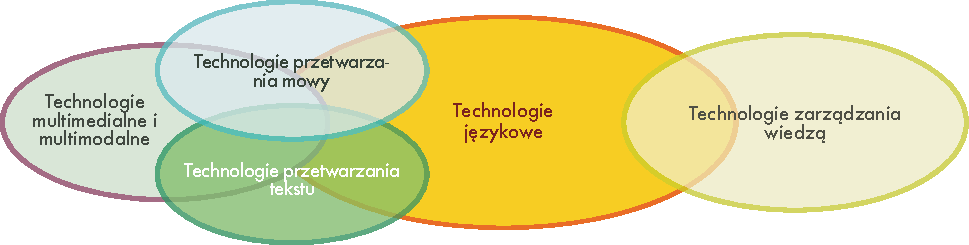
\includegraphics[width=\textwidth]{../_media/polish/language_technologies}
\caption{Technologie językowe} \label{fig: ltincontext_pl}
\colorrule{grey3}{\textwidth}{1.5pt} \end{figure*} 

Technologie językowe to znana dyscyplina badań, w~której istnieje
obszerna literatura wprowadzająca. Zainteresowany czytelnik może
sięgnąć do następujących pozycji bibliograficznych:
\cite{jurafsky-martin01, manning-schuetze1, lt-world1, lt-survey1,
mykowiecka1}. Odnośniki do wspomnianych niżej narzędzi i~zasobów
dla języka polskiego podaje portal \textit{Computational Linguistics
in Poland}~\cite{Clip2}. 

Zanim omówimy powyższe obszary zastosowań, krótko
scharakteryzujemy architekturę typowego systemu TJ. 

\subsection[Architektury aplikacji technologii
językowych]{Architektury aplikacji technologii językowych} Typowe
aplikacje służące do przetwarzania języka składają się z~wielu
komponentów odpowiadających poszczególnym aspektom języka
i~zadaniom, które wykonują. Rysunek~\ref{fig: textprocessingarch_pl}
przedstawia ogólną architekturę systemu przetwarzania tekstu.
Pierwsze trzy moduły odpowiedzialne są za przetwarzanie struktury
i~znaczenia danych wejściowych: 

\begin{itemize} \item Przetwarzanie wstępne: normalizacja danych,
usuwanie formatowania, wykrywanie języka i~kodowania znaków itd.
\item \textbf{Analiza gramatyczna}: wykrywanie orzeczenia i~jego
dopełnień, okoliczników itd.; określanie struktury zdania. \item
\textbf{Analiza semantyczna}: ujednoznacznianie (które ze znaczeń
słowa \emph{wina} jest odpowiednie w~danym kontekście?),
identyfikacja nawiązań (takich jak \emph{ona}, \emph{ten samochód}
itp.); przedstawianie znaczenia zdania w~postaci czytelnej dla
komputera. \end{itemize} 

\begin{figure*}[b] \colorrule{grey3}{\textwidth}{1.5pt} \center
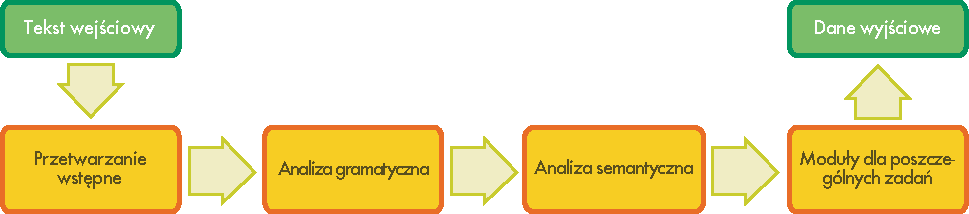
\includegraphics[width=\textwidth]{../_media/polish/text_processing_app_architecture}
\caption{Architektura systemu przetwarzania tekstu} \label{fig:
textprocessingarch_pl} \colorrule{grey3}{\textwidth}{1.5pt}
\end{figure*} 

Moduły przeznaczone do wykonywania poszczególnych zadań mogą
wykonywać takie operacje, jak automatyczne generowanie streszczeń
tekstu wejściowego i~wyszukiwanie w~bazie danych. Poniżej
przedstawione są główne obszary zastosowań wraz z~odpowiadającymi
im modułami. Należy przy tym zaznaczyć, że opisywana architektura
aplikacji jest ogólnym, uproszczonym schematem, mającym na celu
zaprezentowanie złożonych z~natury aplikacji językowych
w~powszechnie zrozumiały sposób. 

Po zaprezentowaniu głównych obszarów zastosowań technologii
językowych przedstawiony zostanie ogólny obraz stanu badań
i~kształcenia w~dziedzinie oraz przegląd (dotychczasowych) zasad
finansowania. Podsumowaniem niniejszego rozdziału jest przygotowane
przez ekspertów zestawienie najważniejszych narzędzi i~zasobów
i~ich ocena na wielu płaszczyznach, takich jak dostępność,
stopień dopracowania lub jakość, dające rzetelny obraz stanu
technologii językowych dla języka polskiego (patrz tabela ~\ref{fig:
lrlttable_pl}). W~tabeli podano wszystkie narzędzia i~zasoby, które
zostały wyróżnione drukiem pogrubionym w~tekście. Technologie
dostępne dla języka polskiego zostały także porównane z~tym, co
jest dostępne dla innych języków omówionych w~tej serii raportów. 

\subsection[Główne obszary zastosowań]{Główne obszary
zastosowań} 

\subsubsection[Korekta językowa]{Korekta językowa} 

Moduły sprawdzania pisowni, wykrywające błędy ortograficzne, są
znane każdemu, kto kiedykolwiek używał edytora tekstu, takiego jak
Microsoft Word. W~ciągu 40 lat, jakie upłynęły od pierwszego
programu do korekty pisowni, stworzonego przez Ralpha Gorrina,
znacznie się one rozwinęły. Dziś nie porównują już listy
wyodrębnionych z~tekstu słów ze słownikiem zawierającym poprawne
formy, lecz wykorzystują dostosowane do poszczególnych języków
algorytmy \textbf{analizy gramatycznej} przetwarzające formy
morfologiczne (np. formy liczby mnogiej), a~niekiedy również
i~błędy składniowe, takie jak brakujące czasowniki lub błędną
liczbę i~rodzaj czasownika, np. w~zdaniu „Ona *pisał list”.
Jednak większość korektorów pisowni nie wykryje błędów
popełnionych specjalnie w~wierszu Jerrolda H.~Zara \cite{zar1}: 

\begin{verse} Eye have a~spelling chequer,\\
It came with my Pea Sea.\\
It plane lee marks four my revue\\
Miss Steaks I~can knot sea. \end{verse} 

Większość dostępnych algorytmów sprawdzania pisowni (w~tym moduł
wbudowany w~program Microsoft Word) nie wykryje w~powyższym
fragmencie błędów, ponieważ analizuje jedynie pojedyncze słowa.
W~wielu przypadkach konieczna jest analiza szerszego kontekstu;
przykładem może być próba określenia, czy słowo „polski”
bądź „Polska” w~poniższych przykładach należy zapisać
wielką, czy małą literą: 

\begin{itemize} \item Ten tekst został przełożony na polski. \item
Czytał „Polskę Zbrojną”. \end{itemize} 

Przypadki takie wymagają sformułowania reguł gramatycznych dla
poszczególnych języków, co wiąże się z~dużymi nakładami pracy
(lub zastosowania metod sztucznej inteligencji), lub użycia
statystycznego modelu języka, obliczającego prawdopodobieństwo
wystąpienia danego słowa w~konkretnym kontekście (np. poprzednich
i~następnych słów), zobacz Rysunek~\ref{fig: langcheckingaarch_pl}.
Fraza „polska książka” będzie na przykład znacznie bardziej
prawdopodobną konstrukcją niż „Polska książka”. Statystyczny
model języka może być stworzony automatycznie przy użyciu dużej
ilości (poprawnych) danych językowych (tzw. \textbf{korpusu}
językowego). 

\begin{figure*}[t] \colorrule{grey3}{\textwidth}{1.5pt} \center

\includegraphics[width=\textwidth]{../_media/polish/language_checking}
\caption{Korekta (regułowa lub statystyczna)} \label{fig:
langcheckingaarch_pl} \colorrule{grey3}{\textwidth}{1.5pt}
\end{figure*} 

Większość prac w~dziedzinie statystycznej korekty językowej
koncentrowała się na metodach i~zasobach dla języka angielskiego,
niekoniecznie przystających do polskiego, który charakteryzuje się
swobodnym szykiem zdania i~bogatą fleksją. Metody oparte na
regułach zostały zaimplementowane w~korektorze LanguageTool,
zawierającym ponad tysiąc reguł dla polskiego (LanguageTool jest
programem o~otwartym kodzie źródłowym przystosowanym do użycia
w~wielu edytorach tekstu, np. LibreOffice) \cite{lto1, Mikowski2010}. 

\boxtext{Moduły sprawdzania poprawności językowej mają
zastosowanie nie tylko w~edytorach tekstu, ale również w~systemach
wspomagających tworzenie dokumentacji.} 

W ostatnich latach znacznie zwiększyła się ilość wytwarzanej
dokumentacji technicznej. Firmy, chcąc uniknąć negatywnych opinii
i~odpowiedzialności prawnej wynikającej z~niezrozumienia przez
klientów instrukcji i~niewłaściwego użycia produktów, zaczęły
coraz bardziej zwracać uwagę na jakość dokumentacji technicznej,
nie zaniedbując przy tym rynku międzynarodowego. Rozwój technologii
przetwarzania języka naturalnego zaowocował powstaniem
oprogramowania wspomagającego tworzenie dokumentacji technicznej,
ułatwiającego jej twórcom używanie słownictwa i~struktur
zdaniowych zgodnych z~określonymi regułami i~(wewnętrznymi)
przepisami regulującymi użycie terminologii. Jako że polszczyzna
rzadko jest językiem źródłowym w~takich zastosowaniach, nie
istnieją jednak systemy opracowane specjalnie dla języka polskiego. 

Poza korektorami i~wspomaganiem tworzenia dokumentacji sprawdzanie
poprawności językowej ma również znaczenie w~dziedzinie nauczania
wspomaganego komputerowo oraz jest stosowanie do autokorekty zapytań
użytkownika w~wyszukiwarkach WWW (np. podpowiedzi „Czy chodziło Ci
o~\ldots{}” w~wyszukiwarce Google). 

\subsubsection[Wyszukiwarki WWW]{Wyszukiwarki WWW} Wyszukiwarka
Google, powstała w~1998~r., obsługuje dziś ok. 80 proc. wszystkich
zapytań \cite{spi1}. Ani interfejs wyszukiwania, ani sposób
prezentacji wyników nie zmieniły się zasadniczo w~porównaniu
z~pierwszą wersją. Obecnie Google oferuje sugestie poprawnej pisowni
błędnie wpisanych terminów; od 2009~r. algorytmy wyszukiwarki
zawierają również podstawowy komponent wyszukiwania semantycznego
\cite{pc1}, umożliwiający podniesienie jakości wyników
wyszukiwania poprzez analizę znaczenia wyszukiwanych terminów
w~kontekście. Sukces firmy Google pokazuje, że przy dostępności
dużej ilości danych i~wydajnych mechanizmach ich indeksowania
podejście w~dużej mierze statystyczne może przynieść
satysfakcjonujące wyniki. 

\begin{figure*}[htb] \colorrule{grey3}{\textwidth}{1.5pt} \center
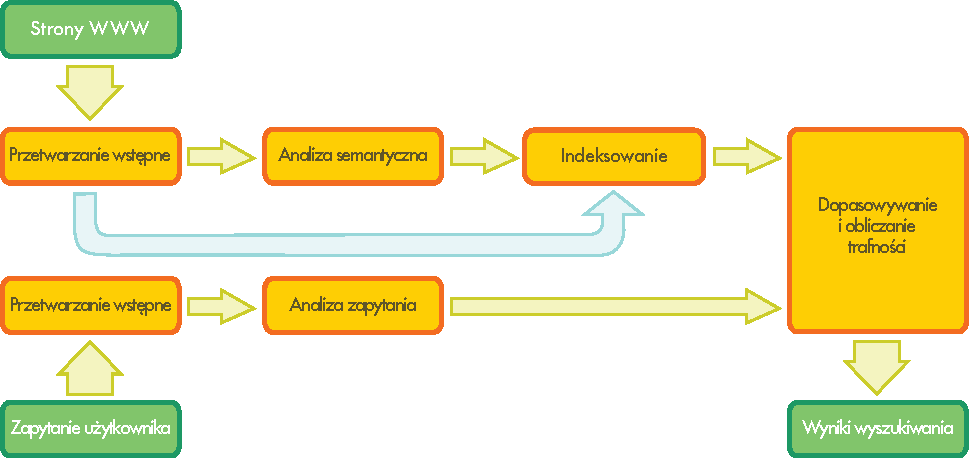
\includegraphics[width=\textwidth]{../_media/polish/web_search_architecture}
\caption{Wyszukiwarka} \label{fig: websearcharch_pl}
\colorrule{grey3}{\textwidth}{1.5pt} \end{figure*} 

Zaspokojenie bardziej złożonych potrzeb informacyjnych wymaga jednak
wykorzystania większych zasobów wiedzy językowej. Prowadzone
w~laboratoriach badawczych eksperymenty wykorzystujące komputerowe
tezaurusy i~zasoby ontologiczne (takie jak WordNet, lub jego polski
odpowiednik, Słowosieć \cite{Slowosiec1, Piasecki2009}) przyniosły
poprawę wyników wyszukiwania przez zwracanie stron zawierających
synonimy wyszukiwanego terminu (np. „energia atomowa”, „energia
jądrowa”, „energia nuklearna” itd.) lub terminy jeszcze
luźniej powiązane. 

\boxtext{Następna generacja wyszukiwarek będzie musiała opierać
się na znacznie bardziej zaawansowanych technologiach językowych.} 

Jeśli wyszukiwana fraza nie jest listą słów kluczowych, lecz
pytaniem lub innym typem zdania, wygenerowanie właściwych odpowiedzi
wymaga analizy składniowej i~semantycznej podanego zdania, jak
również istnienia indeksu umożliwiającego szybkie wyszukanie
odpowiednich dokumentów. Wyobraźmy sobie, że użytkownik wpisuje
zapytanie „Podaj mi listę firm przejętych przez inne firmy
w~ciągu ostatnich pięciu lat”; wymaga ono zastosowania
\textbf{analizy składniowej} i~\textbf{semantycznej}, aby móc
zanalizować strukturę gramatyczną podanego zdania i~określić, że
użytkownik poszukuje firm, które zostały przejęte, a~nie firm,
które przejęły inne firmy. Należy również zanalizować
wyrażenie \emph{ostatnie pięć lat}, aby określić, do którego
roku odnosi się zapytanie. Przetwarzane zapytanie musi wreszcie
zostać dopasowane do dużej ilości nieuporządkowanych danych, aby
odnaleźć informację lub informacje, których poszukuje użytkownik.
Wymaga to zaimplementowania systemu wyszukiwawczego oraz systemu
klasyfikacji wyników. Tworzenie listy firm wymaga dodatkowo wykrycia,
że konkretny ciąg znaków odpowiada nazwie firmy; za tego typu
informacje odpowiadają systemy identyfikacji bytów nazwanych. 

Jeszcze większym wyzwaniem jest wyszukiwanie dokumentów
odpowiadających zapytaniu zadanemu w~innym języku. W~wyszukiwaniu
wielojęzycznym zapytanie musi zostać automatycznie przetłumaczone
na wszystkie możliwe języki źródłowe, a~wyszukane informacje –
z~powrotem na język docelowy. 

Rosnąca ilość danych zapisanych w~formatach innych niż tekst
tworzy zapotrzebowanie na usługi oferujące wyszukiwanie
multimedialne, tj. wyszukiwanie informacji w~danych graficznych,
dźwiękowych i~wideo. W~przypadku danych dźwiękowych i~wideo wymaga
to stworzenia modułu rozpoznawania mowy, przetwarzającego dane
mówione na tekst lub ich reprezentację fonetyczną, w~których może
zostać zrealizowane zapytanie użytkownika. 

Polskie małe i~średnie przedsiębiorstwa, takie jak poznański
Carrot Search, z~powodzeniem rozwijają i~implementują technologie
wyszukiwania zwracające wyniki wyszukiwania bardziej uporządkowane
niż w~standardowych wyszukiwarkach (np. Google) dzięki zastosowaniu
metod grupowania wyników dostosowanych do poszczególnych języków.
Znaczącymi polskimi wyszukiwarkami są NetSprint oraz Szukacz,
zintegrowany z~polskim tezaurusem i~przeprowadzający normalizację
morfologiczną tekstu, co poprawia wyniki wyszukiwania. 

\subsubsection[Interakcja głosowa]{Interakcja głosowa} 

Technologie interakcji głosowej stanowią podstawę dla interfejsów
umożliwiających użytkownikom głosową \ obsługę urządzeń (bez
pomocy myszki, klawiatury czy ekranu). Głosowe interfejsy
użytkownika są obecnie stosowane w~częściowo lub w~pełni
zautomatyzowanych usługach świadczonych przez firmy telefonicznie
klientom, pracownikom i~partnerom biznesowym. 

\boxtext{Interfejsy głosowe są często stosowane w~sektorach takich
jak bankowość, logistyka, transport publiczny i~telekomunikacja.} 

Technologia przetwarzania głosu stosowana jest także w~interfejsach
do konkretnych urządzeń, np. w~systemach nawigacji samochodowej
i~w~graficznych interfejsach użytkownika, np. w~nowoczesnych
telefonach komórkowych (tzw. smartfonach). 

\begin{figure*}[htb] \colorrule{grey3}{\textwidth}{1.5pt} \center
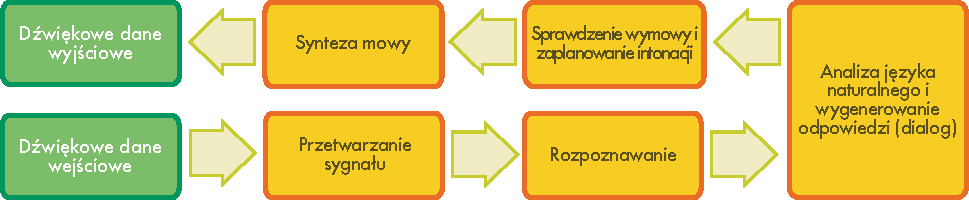
\includegraphics[width=\textwidth]{../_media/polish/simple_speech-based_dialogue_architecture}
\caption{Interakcja głosowa} \label{fig: dialoguearch_pl}
\colorrule{grey3}{\textwidth}{1.5pt} \end{figure*} 

U podstaw interakcji głosowej leżą cztery technologie: 

\begin{itemize} \item Automatyczne \textbf{rozpoznawanie mowy}
umożliwia automatyczne przetworzenie ciągu głosek wypowiadanych
przez użytkownika systemu na konkretne słowa. \item Analiza
gramatyczna i~analiza semantyczna odpowiadają za analizę struktury
składniowej i~znaczeniowej wypowiedzi użytkownika na potrzeby danego
systemu. \item Systemy dialogowe pozwalają zinterpretować żądanie
użytkownika i~podjąć odpowiednie działania. \item \textbf{Synteza
mowy} polega na przetworzeniu pisemnej postaci wypowiedzi na postać
dźwiękową. \end{itemize} 

Jednym z~głównych wyzwań stojących przed automatycznym
rozpoznawaniem mowy jest rozpoznanie słów wypowiedzianych przez
użytkownika z~maksymalną możliwą precyzją. Wymaga to ograniczenia
zakresu możliwych wypowiedzi do zbioru wybranych słów kluczowych
lub ręcznego utworzenia modelu języka na podstawie \textbf{korpusu
języka mówionego}, czyli ze zbiorów plików dźwiękowych
z~nagraniami mowy wraz z~ich tekstowymi transkrypcjami. Pierwsze
z~powyższych rozwiązań skutkuje ograniczoną elastycznością
powstałego przy takich założeniach interfejsu głosowego i~może
pogorszyć ocenę produktu, ale koszty stworzenia, kalibracji
i~administrowania modeli językowych mogą być znaczne. Natomiast
interfejsy używające modeli językowych i~dające użytkownikom
większą swobodę w~wyrażaniu swoich potrzeb – na przykład
poprzez zapytanie \emph{Jak mogę pomóc?} – umożliwiają dużo
większe zautomatyzowanie systemu i~w~rezultacie są znacznie wyżej
oceniane przez użytkowników, a~zatem mogą być uznawane za
korzystniejsze niż bardziej ograniczone systemy oparte na dialogu
kierowanym. 

Większość stosowanych w~praktyce systemów syntezy mowy bazuje na
nagranych uprzednio wypowiedziach. Takie rozwiązanie może
w~zupełności wystarczać w~przypadku wypowiedzi statycznych,
niezależnych od konkretnego kontekstu użycia lub podanych przez
użytkownika danych. Im bardziej jednak dynamiczna jest zawartość
wypowiedzi, tym jakość systemu będzie niższa ze względu na
mechaniczne łączenie przez system pojedynczych plików
dźwiękowych, a~co za tym idzie, nienaturalną intonację i~akcent
wyrazowy wypowiedzi. W~przeciwieństwie do systemów statycznych
metody syntezy mowy umożliwiają osiągnięcie dużo wyższej
jakości i~wytworzenie naturalniej (choć ciągle nie idealnie)
brzmiących wypowiedzi. 

\boxtext{Interakcja głosowa to podstawa interfejsów pozwalających
użytkownikowi obsługę przy użyciu języka mówionego.} 

W ciągu ostatnich dziesięciu lat na rynku technologii interakcji
głosowej można było zaobserwować rosnącą standaryzację
interfejsów stosowanych w~różnych komponentach oraz ujednolicenie
zasad tworzenia poszczególnych składników danej aplikacji.
Nastąpiła również daleko idąca konsolidacja rynku, szczególnie
w~zakresie automatycznego rozpoznawania i~syntezy mowy – rynki
lokalne krajów grupy G20 (tj. silnych gospodarczo krajów
o~znaczącej liczbie ludności) zostały zdominowane przez kilka
globalnych firm; w~Europie najważniejszymi z~nich są Nuance
i~Loquendo. 

Na polskim rynku syntezy mowy najważniejszym graczem jest Ivona,
mająca w~ofercie również produkty dla innych języków. Sytuacja
przedstawia się inaczej w~przypadku języków o~mniejszej liczbie
użytkowników – komercyjne systemy rozpoznawania i~syntezy mowy
często są dla nich niedostępne. W~przypadku technologii i~wiedzy
eksperckiej z~zakresu systemów dialogowych rynki są
w~przeważającej większości zdominowane przez lokalne,
najczęściej małe i~średnie przedsiębiorstwa. W~Polsce głównymi
graczami są obecnie PrimeSpeech i~Skrybot, których model biznesowy
przewiduje nie tylko sprzedaż licencji na oprogramowanie, ale też
dostarczanie kompleksowych rozwiązań wykorzystujących systemy
rozpoznawania mowy. Trudno na razie mówić o~rynku dla technologii
analizy składniowej i~semantycznej w~zakresie interakcji głosowej. 

Jeśli chodzi o~faktyczne wykorzystanie interfejsów głosowych, popyt
na nie znacząco wzrósł w~Polsce w~ciągu ostatnich 5 lat. Główną
przyczyną tego zjawiska było rosnące zapotrzebowanie wśród
użytkowników końcowych na rozwiązania oferujące możliwość
samoobsługi, jak również konieczność optymalizacji kosztów
w~przypadku zautomatyzowanych usług telefonicznych oraz wzrost
akceptacji wśród klientów dla głosowej komunikacji z~maszyną. 

Wybiegając w~przyszłość, można przewidzieć znaczące zmiany
związane z~coraz powszechniejszym użyciem smartfonów, obok
telefonu, Internetu i~poczty elektronicznej, jako platformy
komunikacji z~klientem. Tendencja ta będzie miała wpływ również
na stopień wykorzystania technologii interakcji głosowej. Po
pierwsze, w~perspektywie długoterminowej zapotrzebowanie na głosowe
interfejsy użytkownika w~telefonii wzrośnie. Po drugie, coraz
istotniejsze jest użycie języka mówionego jako łatwej w~użytku
formy pracy z~urządzeniami. Już teraz można zauważyć zwiększenie
precyzji systemów rozpoznawania mowy stosowanych w~smartfonach, co
stało się możliwe głównie dzięki przeniesieniu funkcji
rozpoznawania mowy do zdalnych ośrodków przetwarzania. Z~tych
wszystkich względów zastosowanie technologii językowych
w~przyszłości powinno znacznie zyskać na znaczeniu. 

\subsubsection[Tłumaczenie maszynowe]{Tłumaczenie maszynowe} 

Idea wykorzystania maszyn cyfrowych do tłumaczenia języka
naturalnego została przedstawiona po raz pierwszy przez A.~D.~Bootha
w~1946~r. W~latach 50. i~na początku lat 80. na badania w~tej
dziedzinie przeznaczono znaczne środki. Niemniej jednak systemy
\textbf{tłumaczenia maszynowego} ciągle jeszcze nie spełniają
oczekiwań, jakie rozbudziły w~pierwszych latach swojego istnienia. 

\begin{figure*}[htb] \colorrule{grey3}{\textwidth}{1.5pt} \center
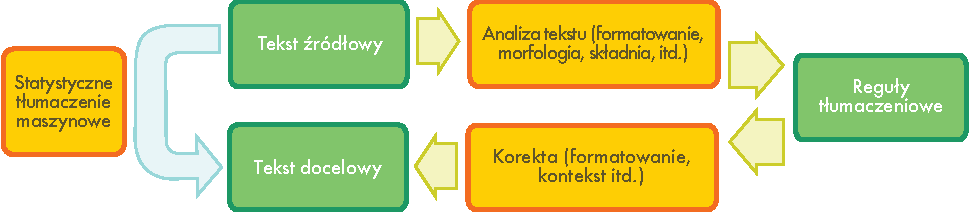
\includegraphics[width=\textwidth]{../_media/polish/machine_translation}
\caption{Tłumaczenie maszynowe (statystyczne, regułowe)} \label{fig:
mtarch_pl} \colorrule{grey3}{\textwidth}{1.5pt} \end{figure*} 

\boxtext{Najprostszą metodą przekładu jest tłumaczenie słowo po
słowie.} 

Na najbardziej podstawowym poziomie tłumaczenie maszynowe polega na
prostym zastąpieniu słów w~jednym języku odpowiadającymi im
słowami w~innym. Algorytmy takie mogą mieć praktyczne zastosowanie
w~dziedzinach o~bardzo ograniczonym, sformalizowanym języku, np.
w~prognozach pogody. Dobrej jakości tłumaczenie większych jednostek
niekonwencjonalnych typów tekstów wymaga jednak dopasowania tekstu
źródłowego do jego najbliższego odpowiednika w~języku docelowym
na poziomie całych wyrażeń, zdań lub dłuższych fragmentów.
Największa trudność wynika tu z~wieloznaczności języka
naturalnego, utrudniającej automatyczne tłumaczenie na wielu
poziomach; na poziomie leksykalnym występuje np. problem
ujednoznaczniania sensu wyrazów („jaguar” może oznaczać
zwierzę lub samochód); na poziomie składniowym – przypisania
przyimków do właściwej części zdania, np.: 

\begin{verse} \textit{Policjant zauważył samochód w~zaroślach.}\\
\textit{Policjant zauważył samochód w~okularach.} \end{verse} 

Jedna z~obecnie stosowanych metod tłumaczenia maszynowego
wykorzystuje algorytmy oparte na regułach językowych. Dla blisko
spokrewnionych ze sobą języków dosłowne tłumaczenie przypadków
takich, jak przedstawiony powyżej, może przynieść akceptowalne
efekty. Często jednak systemy oparte na regułach analizują tekst
źródłowy i~generują pośrednią, symboliczną jego reprezentację,
na podstawie której tworzony jest tekst docelowy. Efektywność
powyższych metod w~wysokim stopniu zależy od dostępności
obszernych leksykonów, zawierających informacje morfologiczne,
składniowe i~semantyczne, oraz dużych zestawów reguł gramatycznych
opartych na wyspecjalizowanej wiedzy językoznawczej. 

Począwszy od lat 80., wraz ze wzrostem możliwości obliczeniowych
komputerów, na znaczeniu zyskały modele statystyczne służące do
tłumaczenia maszynowego, tworzone na podstawie analizy
dwujęzycznych, lub \textbf{równoległych}, \textbf{korpusów}
tekstów (takich jak korpus równoległy Europarl, zawierający
protokoły z~prac Parlamentu Europejskiego w~21 językach UE). Przy
wystarczającej ilości danych tłumaczenie statystyczne jest często
w~stanie przedstawić przybliżone znaczenie tekstu.
W~przeciwieństwie jednak do systemów regułowych tłumaczenie
statystyczne (oparte na danych) często generuje teksty
niegramatyczne. Natomiast przewagą systemów statystycznych, poza
niższym kosztem korekty gramatycznej w~porównaniu z~tłumaczeniem,
jest to, iż mogą poprawnie przetłumaczyć problematyczne fragmenty
wynikające z~indywidualnych cech danego języka, na przykład
wyrażenia idiomatyczne. 

Ponieważ omawiane tu typy systemów tłumaczenia maszynowego
wzajemnie się uzupełniają, obecnie większość badań prowadzona
jest nad systemami hybrydowymi, łączącymi w~sobie obydwie
metodologie (zobacz Rysunek~\ref{fig: mtarch_pl}). Można to
osiągnąć na wiele sposobów. Jednym z~nich jest wykorzystywanie
zarówno systemu opartego na wiedzy, jak i~na danych,
i~zaimplementowanie modułu dokonującego wyboru najlepszego
tłumaczenia. Dla dłuższych zdań jednak żaden z~wyników nie
będzie doskonały. Lepszym rozwiązaniem jest więc połączenie
tłumaczeń poszczególnych części zdania pochodzących z~różnych
źródeł; może być to zadaniem dość złożonym, jako że
zidentyfikowanie odpowiadających sobie fragmentów w~poszczególnych
alternatywnych tłumaczeniach może być trudne. 

\boxtext{W przypadku języka polskiego tłumaczenie maszynowe jest
zadaniem szczególnie trudnym.} 

Tłumaczenie maszynowe tekstu polskiego jest zadaniem wyjątkowo
trudnym. Swobodny szyk zdania utrudnia analizę, a~bogata fleksja –
generowanie poprawnych form gramatycznych. 

Najważniejszym systemem tłumaczenia maszynowego w~Polsce jest
szeroko stosowana Translatica (rozwijana przez firmę Poleng
\cite{Jassem2006}), powstająca we współpracy z~PWN
i~wykorzystująca wydawane przez nie słowniki, w~tym polsko-angielski
słownik PWN-Oxford. Translatica jest systemem \textbf{opartym na
regułach}, obsługującym język polski, angielski, niemiecki
i~rosyjski. Liczne projekty badawcze w~zakresie systemów
statystycznych i~hybrydowych nie zaowocowały na razie komercyjnie
udanym produktem. 

Język polski obsługiwany jest również przez zwykłe
\textbf{statystyczne} systemy tłumaczenia maszynowego, takie jak
Google Translate czy Bing, które sprawdzają się szczególnie
w~tłumaczeniu tekstów polskich na język angielski i~angielskich na
język polski. W~przypadku innych języków jakość tłumaczenia jest
znacznie gorsza, a~wyniki często bywają niezrozumiałe lub wręcz
absurdalne. U~podstaw takiego stanu rzeczy leży mała dostępność
korpusów równoległych, niezbędnych do uczenia systemów
statystycznych. 

Systemy tłumaczenia maszynowego umożliwiające wykorzystanie
wewnętrznej terminologii i~integrację z~systemami zarządzania
projektem mogą znacznie zwiększyć wydajność pracy tłumaczy. Na
rynku polskim funkcjonują specjalne systemy wspomagające proces
tłumaczenia, np. TranslAide firmy Poleng czy TIGER, stworzony przez
Studio Gambit; istnieją również tworzone przez mniejsze MŚP
narzędzia do tłumaczenia wspomaganego komputerowo, takie jak
Cafetran. Ważnym narzędziem jest również system Thetos,
tłumaczący polski na język migowy. 

Jakość systemów tłumaczenia maszynowego pozostawia nadal bardzo
wiele do życzenia. Nierozwiązane jeszcze problemy obejmują
możliwość adaptacji zasobów językowych do poszczególnych
dziedzin oraz integrację z~istniejącymi systemami zarządzania
tłumaczeniami oraz bazami terminologii i~pamięciami
tłumaczeniowymi. Większość z~obecnych systemów jest ponadto
rozwijana głównie dla tłumaczenia między polskim a~angielskim;
obsługa innych kombinacji językowych jest ograniczona. Prowadzi to
do zaburzenia i~spowolnienia procesu tłumaczenia, np. zmuszając
użytkowników systemów tłumaczenia maszynowego do przyswojenia
sobie różnych schematów kodowania terminologii dla różnych
systemów. 

Kampanie na rzecz ewaluacji pomagają porównywać jakość systemów
tłumaczenia maszynowego, różne podejścia i~stan tych systemów dla
różnych par języków. Tabela~\ref{fig: euromatrix_pl} (s.
\pageref{fig: euromatrix_pl}), która została przygotowana w~trakcie
projektu Euromatrix+, zawiera wyniki dla par uzyskane dla 22 z~23
języków urzędowych UE (irlandzki nie był porównywany). Wyniki są
uszeregowane według wyniku BLEU, a~wyższe wyniki oznaczają lepsze
tłumaczenia \cite{bleu1}. Tłumacz będący człowiekiem zazwyczaj
osiąga wynik na poziomie około 80 punktów. 

Najlepsze wyniki (w~kolorze zielonym i~niebieskim) mają języki
korzystające ze znacznych wysiłków w~ramach skoordynowanych
programów oraz mające wiele korpusów równoległych (np. angielski,
francuski, niderlandzki, hiszpański i~niemiecki). Języki o~gorszych
wynikach przedstawiono w~kolorze czerwonym. W~odniesieniu do nich nie
ma takich programów lub są one strukturalnie bardzo różne od
innych języków (np. węgierski, maltański i~fiński). 

\begin{figure*}[htbp]
  \centering
  \setlength{\tabcolsep}{0.17em}
  \small
  \begin{tabular}{>{\columncolor{corange1}}cccccccccccccccccccccccc}
    & \multicolumn{22}{>{\columncolor{corange1}}c}{Język docelowy -- \textcolor{grey1}{Target language}}\\\addlinespace[{-.009cm}]
    \rowcolor{corange1}  & EN & BG & DE & CS & DA & EL & ES & ET & FI & FR & HU & IT & LT & LV & MT & NL & PL & PT & RO & SK & SL & SV\\
    EN & -- & \textcolor{blue}{40.5} & \textcolor{blue}{46.8} & \textcolor{green2}{52.6} & \textcolor{green2}{50.0} & \textcolor{blue}{41.0} & \textcolor{green2}{55.2} & \textcolor{purple}{34.8} & \textcolor{purple}{38.6} & \textcolor{green2}{50.1} & \textcolor{purple}{37.2} & \textcolor{green2}{50.4} & \textcolor{purple}{39.6} & \textcolor{blue}{43.4} & \textcolor{purple}{39.8} & \textcolor{green2}{52.3} & \textcolor{blue}{49.2} & \textcolor{green2}{55.0} & \textcolor{blue}{49.0} & \textcolor{blue}{44.7} & \textcolor{green2}{50.7} & \textcolor{green2}{52.0}\\
    BG & \textcolor{green}{61.3} & -- & \textcolor{purple}{38.7} & \textcolor{purple}{39.4} & \textcolor{purple}{39.6} & \textcolor{purple}{34.5} & \textcolor{blue}{46.9} & \textcolor{red3}{25.5} & \textcolor{red3}{26.7} & \textcolor{blue}{42.4} & \textcolor{red3}{22.0} & \textcolor{blue}{43.5} & \textcolor{red3}{29.3} & \textcolor{red3}{29.1} & \textcolor{red3}{25.9} & \textcolor{blue}{44.9} & \textcolor{purple}{35.1} & \textcolor{blue}{45.9} & \textcolor{purple}{36.8} & \textcolor{purple}{34.1} & \textcolor{purple}{34.1} & \textcolor{purple}{39.9}\\
    DE & \textcolor{green2}{53.6} & \textcolor{red3}{26.3} & -- & \textcolor{purple}{35.4} & \textcolor{blue}{43.1} & \textcolor{purple}{32.8} & \textcolor{blue}{47.1} & \textcolor{red3}{26.7} & \textcolor{red3}{29.5} & \textcolor{purple}{39.4} & \textcolor{red3}{27.6} & \textcolor{blue}{42.7} & \textcolor{red3}{27.6} & \textcolor{purple}{30.3} & \textcolor{red2}{19.8} & \textcolor{green2}{50.2} & \textcolor{purple}{30.2} & \textcolor{blue}{44.1} & \textcolor{purple}{30.7} & \textcolor{red3}{29.4} & \textcolor{purple}{31.4} & \textcolor{blue}{41.2}\\
    CS & \textcolor{green2}{58.4} & \textcolor{purple}{32.0} & \textcolor{blue}{42.6} & -- & \textcolor{blue}{43.6} & \textcolor{purple}{34.6} & \textcolor{blue}{48.9} & \textcolor{purple}{30.7} & \textcolor{purple}{30.5} & \textcolor{blue}{41.6} & \textcolor{red3}{27.4} & \textcolor{blue}{44.3} & \textcolor{purple}{34.5} & \textcolor{purple}{35.8} & \textcolor{red3}{26.3} & \textcolor{blue}{46.5} & \textcolor{purple}{39.2} & \textcolor{blue}{45.7} & \textcolor{purple}{36.5} & \textcolor{blue}{43.6} & \textcolor{blue}{41.3} & \textcolor{blue}{42.9}\\
    DA & \textcolor{green2}{57.6} & \textcolor{red3}{28.7} & \textcolor{blue}{44.1} & \textcolor{purple}{35.7} & -- & \textcolor{purple}{34.3} & \textcolor{blue}{47.5} & \textcolor{red3}{27.8} & \textcolor{purple}{31.6} & \textcolor{blue}{41.3} & \textcolor{red3}{24.2} & \textcolor{blue}{43.8} & \textcolor{red3}{29.7} & \textcolor{purple}{32.9} & \textcolor{red3}{21.1} & \textcolor{blue}{48.5} & \textcolor{purple}{34.3} & \textcolor{blue}{45.4} & \textcolor{purple}{33.9} & \textcolor{purple}{33.0} & \textcolor{purple}{36.2} & \textcolor{blue}{47.2}\\
    EL & \textcolor{green2}{59.5} & \textcolor{purple}{32.4} & \textcolor{blue}{43.1} & \textcolor{purple}{37.7} & \textcolor{blue}{44.5} & -- & \textcolor{green2}{54.0} & \textcolor{red3}{26.5} & \textcolor{red3}{29.0} & \textcolor{blue}{48.3} & \textcolor{red3}{23.7} & \textcolor{blue}{49.6} & \textcolor{red3}{29.0} & \textcolor{purple}{32.6} & \textcolor{red3}{23.8} & \textcolor{blue}{48.9} & \textcolor{purple}{34.2} & \textcolor{green2}{52.5} & \textcolor{purple}{37.2} & \textcolor{purple}{33.1} & \textcolor{purple}{36.3} & \textcolor{blue}{43.3}\\
    ES & \textcolor{green}{60.0} & \textcolor{purple}{31.1} & \textcolor{blue}{42.7} & \textcolor{purple}{37.5} & \textcolor{blue}{44.4} & \textcolor{purple}{39.4} & -- & \textcolor{red3}{25.4} & \textcolor{red3}{28.5} & \textcolor{green2}{51.3} & \textcolor{red3}{24.0} & \textcolor{green2}{51.7} & \textcolor{red3}{26.8} & \textcolor{purple}{30.5} & \textcolor{red3}{24.6} & \textcolor{blue}{48.8} & \textcolor{purple}{33.9} & \textcolor{green2}{57.3} & \textcolor{purple}{38.1} & \textcolor{purple}{31.7} & \textcolor{purple}{33.9} & \textcolor{blue}{43.7}\\
    ET & \textcolor{green2}{52.0} & \textcolor{red3}{24.6} & \textcolor{purple}{37.3} & \textcolor{purple}{35.2} & \textcolor{purple}{37.8} & \textcolor{red3}{28.2} & \textcolor{blue}{40.4} & -- & \textcolor{purple}{37.7} & \textcolor{purple}{33.4} & \textcolor{purple}{30.9} & \textcolor{purple}{37.0} & \textcolor{purple}{35.0} & \textcolor{purple}{36.9} & \textcolor{red3}{20.5} & \textcolor{blue}{41.3} & \textcolor{purple}{32.0} & \textcolor{purple}{37.8} & \textcolor{red3}{28.0} & \textcolor{purple}{30.6} & \textcolor{purple}{32.9} & \textcolor{purple}{37.3}\\
    FI & \textcolor{blue}{49.3} & \textcolor{red3}{23.2} & \textcolor{purple}{36.0} & \textcolor{purple}{32.0} & \textcolor{purple}{37.9} & \textcolor{red3}{27.2} & \textcolor{purple}{39.7} & \textcolor{purple}{34.9} & -- & \textcolor{red3}{29.5} & \textcolor{red3}{27.2} & \textcolor{purple}{36.6} & \textcolor{purple}{30.5} & \textcolor{purple}{32.5} & \textcolor{red2}{19.4} & \textcolor{blue}{40.6} & \textcolor{red3}{28.8} & \textcolor{purple}{37.5} & \textcolor{red3}{26.5} & \textcolor{red3}{27.3} & \textcolor{red3}{28.2} & \textcolor{purple}{37.6}\\
    FR & \textcolor{green}{64.0} & \textcolor{purple}{34.5} & \textcolor{blue}{45.1} & \textcolor{purple}{39.5} & \textcolor{blue}{47.4} & \textcolor{blue}{42.8} & \textcolor{green}{60.9} & \textcolor{red3}{26.7} & \textcolor{purple}{30.0} & -- & \textcolor{red3}{25.5} & \textcolor{green2}{56.1} & \textcolor{red3}{28.3} & \textcolor{purple}{31.9} & \textcolor{red3}{25.3} & \textcolor{green2}{51.6} & \textcolor{purple}{35.7} & \textcolor{green}{61.0} & \textcolor{blue}{43.8} & \textcolor{purple}{33.1} & \textcolor{purple}{35.6} & \textcolor{blue}{45.8}\\
    HU & \textcolor{blue}{48.0} & \textcolor{red3}{24.7} & \textcolor{purple}{34.3} & \textcolor{purple}{30.0} & \textcolor{purple}{33.0} & \textcolor{red3}{25.5} & \textcolor{purple}{34.1} & \textcolor{red3}{29.6} & \textcolor{red3}{29.4} & \textcolor{purple}{30.7} & -- & \textcolor{purple}{33.5} & \textcolor{red3}{29.6} & \textcolor{purple}{31.9} & \textcolor{red2}{18.1} & \textcolor{purple}{36.1} & \textcolor{red3}{29.8} & \textcolor{purple}{34.2} & \textcolor{red3}{25.7} & \textcolor{red3}{25.6} & \textcolor{red3}{28.2} & \textcolor{purple}{30.5}\\
    IT & \textcolor{green}{61.0} & \textcolor{purple}{32.1} & \textcolor{blue}{44.3} & \textcolor{purple}{38.9} & \textcolor{blue}{45.8} & \textcolor{blue}{40.6} & \textcolor{red3}{26.9} & \textcolor{red3}{25.0} & \textcolor{red3}{29.7} & \textcolor{green2}{52.7} & \textcolor{red3}{24.2} & -- & \textcolor{red3}{29.4} & \textcolor{purple}{32.6} & \textcolor{red3}{24.6} & \textcolor{green2}{50.5} & \textcolor{purple}{35.2} & \textcolor{green2}{56.5} & \textcolor{purple}{39.3} & \textcolor{purple}{32.5} & \textcolor{purple}{34.7} & \textcolor{blue}{44.3}\\
    LT & \textcolor{green2}{51.8} & \textcolor{red3}{27.6} & \textcolor{purple}{33.9} & \textcolor{purple}{37.0} & \textcolor{purple}{36.8} & \textcolor{red3}{26.5} & \textcolor{red3}{21.1} & \textcolor{purple}{34.2} & \textcolor{purple}{32.0} & \textcolor{purple}{34.4} & \textcolor{red3}{28.5} & \textcolor{purple}{36.8} & -- & \textcolor{blue}{40.1} & \textcolor{red3}{22.2} & \textcolor{purple}{38.1} & \textcolor{purple}{31.6} & \textcolor{purple}{31.6} & \textcolor{red3}{29.3} & \textcolor{purple}{31.8} & \textcolor{purple}{35.3} & \textcolor{purple}{35.3}\\
    LV & \textcolor{green2}{54.0} & \textcolor{red3}{29.1} & \textcolor{purple}{35.0} & \textcolor{purple}{37.8} & \textcolor{purple}{38.5} & \textcolor{red3}{29.7} & \textcolor{red2}{8.0} & \textcolor{purple}{34.2} & \textcolor{purple}{32.4} & \textcolor{purple}{35.6} & \textcolor{red3}{29.3} & \textcolor{purple}{38.9} & \textcolor{purple}{38.4} & -- & \textcolor{red3}{23.3} & \textcolor{blue}{41.5} & \textcolor{purple}{34.4} & \textcolor{purple}{39.6} & \textcolor{purple}{31.0} & \textcolor{purple}{33.3} & \textcolor{purple}{37.1} & \textcolor{purple}{38.0}\\
    MT & \textcolor{green}{72.1} & \textcolor{purple}{32.2} & \textcolor{purple}{37.2} & \textcolor{purple}{37.9} & \textcolor{purple}{38.9} & \textcolor{purple}{33.7} & \textcolor{blue}{48.7} & \textcolor{red3}{26.9} & \textcolor{red3}{25.8} & \textcolor{blue}{42.4} & \textcolor{red3}{22.4} & \textcolor{blue}{43.7} & \textcolor{purple}{30.2} & \textcolor{purple}{33.2} & -- & \textcolor{blue}{44.0} & \textcolor{purple}{37.1} & \textcolor{blue}{45.9} & \textcolor{purple}{38.9} & \textcolor{purple}{35.8} & \textcolor{blue}{40.0} & \textcolor{blue}{41.6}\\
    NL & \textcolor{green2}{56.9} & \textcolor{red3}{29.3} & \textcolor{blue}{46.9} & \textcolor{purple}{37.0} & \textcolor{blue}{45.4} & \textcolor{purple}{35.3} & \textcolor{blue}{49.7} & \textcolor{red3}{27.5} & \textcolor{red3}{29.8} & \textcolor{blue}{43.4} & \textcolor{red3}{25.3} & \textcolor{blue}{44.5} & \textcolor{red3}{28.6} & \textcolor{purple}{31.7} & \textcolor{red3}{22.0} & -- & \textcolor{purple}{32.0} & \textcolor{blue}{47.7} & \textcolor{purple}{33.0} & \textcolor{purple}{30.1} & \textcolor{purple}{34.6} & \textcolor{blue}{43.6}\\
    PL & \textcolor{green}{60.8} & \textcolor{purple}{31.5} & \textcolor{blue}{40.2} & \textcolor{blue}{44.2} & \textcolor{blue}{42.1} & \textcolor{purple}{34.2} & \textcolor{blue}{46.2} & \textcolor{red3}{29.2} & \textcolor{red3}{29.0} & \textcolor{blue}{40.0} & \textcolor{red3}{24.5} & \textcolor{blue}{43.2} & \textcolor{purple}{33.2} & \textcolor{purple}{35.6} & \textcolor{red3}{27.9} & \textcolor{blue}{44.8} & -- & \textcolor{blue}{44.1} & \textcolor{purple}{38.2} & \textcolor{purple}{38.2} & \textcolor{purple}{39.8} & \textcolor{blue}{42.1}\\
    PT & \textcolor{green}{60.7} & \textcolor{purple}{31.4} & \textcolor{blue}{42.9} & \textcolor{purple}{38.4} & \textcolor{blue}{42.8} & \textcolor{blue}{40.2} & \textcolor{green}{60.7} & \textcolor{red3}{26.4} & \textcolor{red3}{29.2} & \textcolor{green2}{53.2} & \textcolor{red3}{23.8} & \textcolor{green2}{52.8} & \textcolor{red3}{28.0} & \textcolor{purple}{31.5} & \textcolor{red3}{24.8} & \textcolor{blue}{49.3} & \textcolor{purple}{34.5} & -- & \textcolor{purple}{39.4} & \textcolor{purple}{32.1} & \textcolor{purple}{34.4} & \textcolor{blue}{43.9}\\
    RO & \textcolor{green}{60.8} & \textcolor{purple}{33.1} & \textcolor{purple}{38.5} & \textcolor{purple}{37.8} & \textcolor{blue}{40.3} & \textcolor{purple}{35.6} & \textcolor{green2}{50.4} & \textcolor{red3}{24.6} & \textcolor{red3}{26.2} & \textcolor{blue}{46.5} & \textcolor{red3}{25.0} & \textcolor{blue}{44.8} & \textcolor{red3}{28.4} & \textcolor{red3}{29.9} & \textcolor{red3}{28.7} & \textcolor{blue}{43.0} & \textcolor{purple}{35.8} & \textcolor{blue}{48.5} & -- & \textcolor{purple}{31.5} & \textcolor{purple}{35.1} & \textcolor{purple}{39.4}\\
    SK & \textcolor{green}{60.8} & \textcolor{purple}{32.6} & \textcolor{purple}{39.4} & \textcolor{blue}{48.1} & \textcolor{blue}{41.0} & \textcolor{purple}{33.3} & \textcolor{blue}{46.2} & \textcolor{red3}{29.8} & \textcolor{red3}{28.4} & \textcolor{purple}{39.4} & \textcolor{red3}{27.4} & \textcolor{blue}{41.8} & \textcolor{purple}{33.8} & \textcolor{purple}{36.7} & \textcolor{red3}{28.5} & \textcolor{blue}{44.4} & \textcolor{purple}{39.0} & \textcolor{blue}{43.3} & \textcolor{purple}{35.3} & -- & \textcolor{blue}{42.6} & \textcolor{blue}{41.8}\\
    SL & \textcolor{green}{61.0} & \textcolor{purple}{33.1} & \textcolor{purple}{37.9} & \textcolor{blue}{43.5} & \textcolor{blue}{42.6} & \textcolor{purple}{34.0} & \textcolor{blue}{47.0} & \textcolor{purple}{31.1} & \textcolor{red3}{28.8} & \textcolor{purple}{38.2} & \textcolor{red3}{25.7} & \textcolor{blue}{42.3} & \textcolor{purple}{34.6} & \textcolor{purple}{37.3} & \textcolor{purple}{30.0} & \textcolor{blue}{45.9} & \textcolor{purple}{38.2} & \textcolor{blue}{44.1} & \textcolor{purple}{35.8} & \textcolor{purple}{38.9} & -- & \textcolor{blue}{42.7}\\
    SV & \textcolor{green2}{58.5} & \textcolor{red3}{26.9} & \textcolor{blue}{41.0} & \textcolor{purple}{35.6} & \textcolor{blue}{46.6} & \textcolor{purple}{33.3} & \textcolor{blue}{46.6} & \textcolor{red3}{27.4} & \textcolor{purple}{30.9} & \textcolor{purple}{38.9} & \textcolor{red3}{22.7} & \textcolor{blue}{42.0} & \textcolor{red3}{28.2} & \textcolor{purple}{31.0} & \textcolor{red3}{23.7} & \textcolor{blue}{45.6} & \textcolor{purple}{32.2} & \textcolor{blue}{44.2} & \textcolor{purple}{32.7} & \textcolor{purple}{31.3} & \textcolor{purple}{33.5} & --\\
    \end{tabular}
  \caption{Tłumaczenie maszynowe między 22 językami europejskimi -- \textcolor{grey1}{Machine translation between 22 EU-languages \cite{euro1}}}
  \label{fig:euromatrix_pl}
\end{figure*}


\subsubsection[Zarządzanie wiedzą i~technologie
pomocnicze]{Zarządzanie wiedzą i~technologie pomocnicze} 

Tworzenie aplikacji z~zakresu technologii językowych obejmuje wiele
etapów, których rezultaty nie zawsze są bezpośrednio widoczne dla
użytkownika, ale które odgrywają ważną rolę w~systemie. Jako
istotne zagadnienia badawcze stały się odrębnymi dziedzinami
językoznawstwa komputerowego. 

Automatyczne odpowiadanie na pytania jest aktywnie rozwijającym się
obszarem badań, w~którego ramach tworzone są anotowane korpusy
i~organizowane są konkursy. Celem takich systemów jest umożliwienie
przejścia od wyszukiwania opartego na słowach kluczowych (na
których podstawie wyszukiwarka generuje listy potencjalnie
adekwatnych dokumentów) do systemów, które udzielają konkretnej
odpowiedzi na pytanie, np: 

\begin{itemize} 
  \item[] \textit{– Ile lat miał Neil Armstrong,
kiedy stanął na Księżycu?} 
  \item[] \textit{– 38. } 
\end{itemize} 

Choć tego typu zastosowania są w~oczywisty sposób związane
z~opisanym powyżej obszarem wyszukiwania w~sieci, automatyczne
odpowiadanie na pytania jest obecnie ogólnym terminem obejmującym
takie zagadnienia badawcze, jak rozróżnianie poszczególnych typów
pytań i~odpowiedniej adaptacji zachowania systemu, metody analizy
i~porównywania zbiorów dokumentów potencjalnie zawierających
odpowiedź (w~celu pogodzenia sprzecznych odpowiedzi), algorytmy
precyzyjnego wyszukiwania odpowiedzi w~dokumencie przy uwzględnieniu
kontekstu itd. 

Ostatnie z~powyższych zagadnień bezpośrednio łączy się
z~obszarem ekstrakcji informacji niezwykle popularnym w~latach 90.,
gdy w~językoznawstwie komputerowym popularne stały się metody
statystyczne. Wyszukiwanie informacji ma na celu identyfikowanie
konkretnych informacji w~określonych typach dokumentów – np.
wykrywanie podmiotów najaktywniej przejmujących inne spółki na
podstawie doniesień prasowych. Innym z~rozwijanych obecnie
zastosowań jest przetwarzanie raportów o~aktach terroru w~celu
wyodrębnienia z~tekstu informacji o~napastniku, celu, dacie
i~godzinie oraz miejscu zdarzenia, a~także jego rezultatach.
Poszukiwanie standardowych informacji dla konkretnych dziedzin jest
podstawową cechą tego obszaru badawczego – stąd też stanowi on
technologię „pomocniczą”, która musi zostać zintegrowana
z~kompletnym systemem odpowiednim dla konkretnego zadania. 

\boxtext{Technologie językowe często są stosowane za kulisami
większych systemów oprogramowania i~zapewniają istotne funkcje.} 

Dwoma obszarami „granicznymi”, pełniącymi czasem rolę
autonomicznych aplikacji, a~czasem technologii narzędziowych, są
systemy generowania streszczeń i~\textbf{generowania tekstu}. Systemy
streszczania tekstu, wbudowane na przykład w~program Microsoft Word,
oparte są głównie na algorytmach statystycznych, identyfikujących
w~tekście „ważne” wyrazy (tj. wyrazy występujące w~tekście
istotnie częściej niż w~języku ogólnym) i~zawierające je zdania.
Zdania te są następnie oznaczane i~wyodrębniane z~tekstu, tworząc
streszczenie. Najczęściej więc w~praktyce streszczenie tekstu
oznacza sprowadzenie go do podzbioru jego zdań: tak funkcjonują
wszystkie dostępne rozwiązania komercyjne. Alternatywną metodą
jest generowanie \emph{nowych} zdań, tj. tworzenie streszczenia ze
zdań, które nie muszą występować w~tekście źródłowym. Wymaga
to głębszego zrozumienia tekstu, w~związku z~czym wyniki tej grupy
metod są dużo mniej przewidywalne. W~obu przypadkach jednak systemy
generowania tekstu rzadko stanowią autonomiczne aplikacje, będąc
najczęściej elementami większych systemów (np. jako moduły
generowania raportów w~medycznych systemach informacyjnych,
gromadzących i~przetwarzających dane o~pacjentach). 

\boxtext{Narzędzia dla języka polskiego są w~opisanych powyżej
obszarach rozwinięte znacznie gorzej niż ich odpowiedniki dla
języka angielskiego.} 

Narzędzia dla języka polskiego są w~opisanych powyżej obszarach
rozwinięte znacznie gorzej niż ich odpowiedniki dla języka
angielskiego, będące od lat 90. przedmiotem licznych konkursów
naukowych, organizowanych przede wszystkim przez amerykańskie
instytucje DARPA/NIST.~Choć konkursy te umożliwiły znaczny rozwój
technologii, skupiały się głównie na języku angielskim; nawet gdy
obejmowały sekcje wielojęzyczne, język polski nigdy nie był
ważnym elementem tych badań. Równie nieliczne są polskie korpusy
anotowane i~inne zasoby niezbędne do realizacji podobnych zadań.
Systemy generowania streszczeń używające metod czysto
statystycznych są w~wielu przypadkach niezależne od języka,
istnieje więc pewna liczba rozwiązań prototypowych. W~przypadku
generowania tekstu możliwe do wykorzystania moduły są zasadniczo
ograniczone do warstwy powierzchniowej („gramatyki generowania
tekstu”); tak jak w~poprzednim przypadku większość systemów jest
zaprojektowana dla języka angielskiego. Prototypowe implementacje
systemu generowania tekstu powstały podczas tworzenia wspomnianego
wcześniej systemu tłumaczenia maszynowego dla języka migowego
Thetos. 

Powyższe zestawienie nie wyczerpuje zastosowań technologii
językowych. Jednym z~aktywnie rozwijanych obszarów jest wykrywanie
plagiatów, u~którego podstaw leżą metody niezależne od języka,
lecz które może być wzbogacone w~opcje wyszukiwania prostych
parafraz tekstu źródłowego. Najpopularniejszym systemem dla języka
polskiego jest usługa plagiat. pl, używana przez większość
uczelni wyższych do sprawdzania oryginalności prac magisterskich,
jak również do identyfikowania przypadków naruszenia praw
autorskich w~sieci \cite{plagiat1}. 

\subsection[Projekty z~zakresu technologii językowych]{Projekty
z~zakresu technologii językowych} 

Jednym z~najwcześniejszych polskich projektów z~zakresu technologii
językowych był podjęty w~1967~r. wysiłek na rzecz stworzenia
korpusu frekwencyjnego współczesnej polszczyzny o~strukturze
porównywalnej z~anglojęzycznym korpusem Brown University. Zadanie
zrealizował interdyscyplinarny zespół naukowców z~Uniwersytetu
Warszawskiego. Częściowe wyniki projektu zostały opublikowane
w~latach 1972--77, a~ukończony korpus – w~roku 1990. W~kolejnych
latach został on wzbogacony na wielu płaszczyznach, zarówno poprzez
ręczną edycję, jak i~metodami automatycznymi. 

Spośród innych projektów realizowanych we wczesnych latach rozwoju
językoznawstwa komputerowego w~Polsce wymienić należy próby
utworzenia reprezentatywnego słownika morfologicznego polszczyzny.
Jedną z~nich był projekt POLEX (1993--1996), realizowany przez
Uniwersytet Adama Mickiewicza; kolejnym projektem był Słownik
Gramatyczny Języka Polskiego \cite{SGJP}, którego efektem jest
najbardziej obecnie zaawansowany analizator morfologiczny języka
polskiego, Morfeusz. W~2008~r. w~Instytucie Informatyki Stosowanej
Politechniki Wrocławskiej, we współpracy z~Uniwersytetem Adama
Mickiewicza (projekt POLNET) rozpoczęty został projekt plWordNet,
mający na celu zbudowanie polskiej wersji bazy
leksykalno-semantycznej WordNet \cite{Slowosiec1, Piasecki2009}.
Powstała w~jego wyniku baza, stworzona przy użyciu licznych
innowacyjnych półautomatycznych metod wykrywania relacji
semantycznych w~korpusach językowych, jest jedną z~największych na
świecie (niektóre z~kategorii są bogatsze niż w~oryginalnej wersji
Princeton University). 

Innym istotnym projektem korpusowym był korpus IPI PAN, tworzony
w~pierwszej dekadzie XXI wieku w~Instytucie Podstaw Informatyki
Polskiej Akademii Nauk (IPI PAN) \cite{korpus1}. W~tym samym okresie
powstały również dwa inne korpusy języka polskiego – korpus PWN,
używany do prac słownikowych, oraz korpus referencyjny PELCRA,
tworzony w~Zakładzie Językoznawstwa Komputerowego Uniwersytetu
Łódzkiego. Ten ostatni zawiera sporą pulę autentycznych danych
konwersacyjnych. Kontynuacją powyższych projektów był rozpoczęty
pod koniec 2008~r. przez wszystkie trzy instytucje oraz Instytut
Języka Polskiego PAN projekt Narodowego Korpusu Języka Polskiego
(NKJP) \cite{nkjp1}, zawierający część zasobów z~korpusów IPI
PAN, PWN oraz PELCRA.~Celem projektu było stworzenie największego
z~dotychczas istniejących, ponadmiliardowego korpusu języka
polskiego oraz milionowego podkorpusu anotowanego ręcznie na wielu
poziomach, w~zamyśle autorów będącego podstawą do tworzenia
dalszych zasobów językowych (jeden z~wykorzystujących NKJP
projektów stawia sobie za zadanie stworzenie pierwszego banku drzew
składniowych dla języka polskiego przy wykorzystaniu anotacji
gramatycznych korpusu). 

W pierwszej dekadzie XXI wieku rozpoczęte zostały również dwa
projekty zajmujące się zbieraniem korpusów języka mówionego oraz
rozwojem metod przetwarzania dyskursu – LUNA (IPI PAN) oraz
POLINT-112-SMS (UAM). Celem projektu LUNA było usprawnienie
zautomatyzowanych systemów telefonicznych poprzez umożliwienie
spontanicznych i~nieograniczonych interakcji człowiek-maszyna.
Projekt POLINT-112-SMS zajmował się zarządzaniem informacjami
w~sytuacjach krytycznych. Tworzony w~nim system, oparty na danych
tekstowych pochodzących z~wiadomości SMS, ma wspomagać proces
podejmowania decyzji w~centrach zarządzania kryzysowego. Jednym
z~elementów projektowanego systemu jest moduł zarządzania
dialogiem. 

Polskie instytucje naukowe są ponadto zaangażowane w~trwające
obecnie projekty CLARIN, mające na celu stworzenie infrastruktury
technologicznej dla narzędzi i~zasobów językowych, oraz FLaReNet,
ogólnoeuropejskie forum ułatwiające interakcję między
użytkownikami i~twórcami zasobów językowych. Biorą one również
aktywny udział w~pracach projektu META-NET. 

Obecnie prowadzone są ponadto co najmniej 2~duże projekty
finansowane ze środków UE w~ramach programu Innowacyjna Gospodarka
– ATLAS i~NEKST – oraz liczne programy badawcze z~dziedziny
technologii językowych, w~tym finansowane z~Programu Ramowego. 

Niemniej jednak zapewnienie odpowiedniego poziomu wsparcia dla
projektów rozwijających zaawansowane technologie, korpusy i~inne
zasoby językowe wymaga zaangażowania większych środków
finansowych. 

\subsection[Badania i~kształcenie w~dziedzinie technologii
językowych]{Badania i~kształcenie w~dziedzinie technologii
językowych} 

Obecnie w~Polsce wiele uniwersytetów i~ośrodków naukowych -- co
najmniej 12 -- aktywnie uczestniczy w~pracach z~zakresu technologii
językowych i~językoznawstwa komputerowego. Wiele z~nich oferuje
kursy w~tym zakresie \cite{centers1}. 

Poza uniwersytetami główne projekty badawcze prowadzone są
w~Zakładzie Inżynierii Lingwistycznej Instytutu Podstaw Informatyki
PAN. 

Towarzystwami naukowymi aktywnymi w~dziedzinie technologii językowych
są Polskie Towarzystwo Informatyczne i~Polskie Towarzystwo
Fonetyczne. 

Jako dziedzina badań technologie językowe stoją przed
następującymi wyzwaniami: 

\begin{itemize} \item Osoby aktywne w~dziedzinie technologii
językowych należą do różnych społeczności naukowych, spotykają
się na odrębnych konferencjach i~należą do odrębnych towarzystw
naukowych; brakuje wspólnego forum, które mogłoby zgromadzić
wszystkie zainteresowane strony. \item Językoznawstwo komputerowe
w~dalszym ciągu jest postrzegane jako dziedzina „egzotyczna”,
o~nieustalonym miejscu w~systemie kształcenia, w~związku z~czym
rozproszona w~różnych wydziałach (np. wydziałach informatyki lub
filologiach). \item Brak efektu synergii między podejmowanymi
zagadnieniami badawczymi. \end{itemize} 

\subsection[Dostępność narzędzi i~zasobów]{Dostępność
narzędzi i~zasobów} W~poniższej tabeli przedstawiony jest ogólny
obraz bieżącej sytuacji na polu technologii językowych w~Polsce.
Ocena (w~skali 0--6) istniejących narzędzi i~zasobów oparta jest na
eksperckim oszacowaniu na skali od 0 (bardzo niska ocena) do 6 (bardzo
wysoka). 

Lista~\ref{fig: lrlttable_pl} przedstawia najważniejsze wnioski
płynące z~oceny stanu technologii językowych w~Polsce. Do
najważniejszych problemów stojących na przeszkodzie dalszemu
rozwojowi metod automatycznego przetwarzania języka można zaliczyć: 

\begin{itemize} \item Brak korpusów oraz zaawansowanych narzędzi do
przetwarzania języka mówionego dla języka polskiego. Ciągle
trwają prace nad korpusami multimodalnymi. \item Wiele z~dostępnych
zasobów nie jest zgodnych ze standardami – nawet jeśli istnieją,
zapewnienie ich trwałości, czyli możliwości ich utrzymania
w~dłuższym okresie może być trudne lub niemożliwe. Konieczne jest
współpraca i~wspólne inicjatywy standaryzujące dane i~formaty ich
zapisu. \item Analiza semantyczna jest trudniejsza niż składniowa;
analiza semantyczna tekstu jest trudniejsza niż pojedynczych wyrazów
lub zdań. \item Im większy zakres analizy semantycznej dokonywanej
przez narzędzie, tym trudniej jest uzyskać odpowiednie dane;
niezbędne są bardziej intensywne prace nad głęboką analizą.
\item Istniejące standardy w~zakresie semantyki i~kodowania wiedzy
(RDF, OWL itd.) nie mogą w~prosty sposób zostać dostosowane do
wymogów przetwarzania języka naturalnego. \item Narzędzia i~zasoby
dla przetwarzania języka mówionego, w~szczególności syntezy mowy,
są obecnie bardziej rozwinięte niż technologie dla języka
pisanego. \item Dotychczasowe badania zaowocowały stworzeniem
pojedynczych narzędzi o~wysokiej jakości, jednak w~obecnych
warunkach finansowych niemalże niemożliwe jest stworzenie trwałego
i~zgodnego ze standardami rozwiązania. \end{itemize} 

\begin{itemize} \item Brakuje dużych, zrównoważonych
i~ogólnodostępnych korpusów równoległych języka polskiego, w~tym
korpusów równoległych języków pokrewnych (np. czeskiego). \item
Do wielu zastosowań niezbędne są dwu- i~wielojęzyczne słowniki
zawierające nie tylko tłumaczenia, lecz również informacje
o~walencji. Jako że standardowe słowniki zazwyczaj pomijają ten
rodzaj anotacji, należy stworzyć odpowiednie zasoby. \item Do wielu
zastosowań niezbędne są duże, ogólnodostępne zasoby ontologiczne
dla języka polskiego. Obecnie dostępne ontologie są relatywnie
małe i~oparte na ontologii OpenCyc lub polskiej wersji tezaurusa
OpenThesaurus. Polska wersja DBPedii jest w~przygotowaniu.
\end{itemize} 

\begin{figure*}[htb]
\centering
%\begin{tabular}{>{\columncolor{orange1}}p{.33\linewidth}ccccccc} % ORIGINAL
\begin{tabular}{>{\columncolor{orange1}}p{.33\linewidth}@{\hspace*{6mm}}c@{\hspace*{6mm}}c@{\hspace*{6mm}}c@{\hspace*{6mm}}c@{\hspace*{6mm}}c@{\hspace*{6mm}}c@{\hspace*{6mm}}c}
\rowcolor{orange1}
 \cellcolor{white}&\begin{sideways}\makecell[l]{Liczba}\end{sideways}
&\begin{sideways}\makecell[l]{\makecell[l]{Dostępność} }\end{sideways} &\begin{sideways}\makecell[l]{Jakość}\end{sideways}
&\begin{sideways}\makecell[l]{Zakres}\end{sideways} &\begin{sideways}\makecell[l]{Dojrzałość}\end{sideways} &\begin{sideways}\makecell[l]{Trwałość}\end{sideways} &\begin{sideways}\makecell[l]{Elastyczność~~}\end{sideways} \\ \addlinespace
\multicolumn{8}{>{\columncolor{orange2}}l}{Technologie językowe (narzędzia, technologie, aplikacje)} \\ \addlinespace
 Rozpoznawanie mowy &
 1 & 2 & 3 & 4 & 3 & 2 & 4\\ \addlinespace
 Synteza mowy &
 4 & 3 & 6 & 5 & 4 & 4 & 3\\ \addlinespace
 Analiza gramatyczna & 
4 & 4,5 & 4,5 & 4,5 & 4 & 4 & 3\\ \addlinespace
 Analiza semantyczna & 
1 & 1 & 3 & 1 & 1 & 2 & 2\\ \addlinespace
 Generowanie tekstu &
 1 & 1 & 1 & 1 & 1 & 1 & 2\\ \addlinespace
 Tłumaczenie maszynowe &
 3 & 4 & 3 & 3 & 3 & 4 & 3\\ \addlinespace
\multicolumn{8}{>{\columncolor{orange2}}l}{Zasoby językowe (zasoby, dane, bazy wiedzy)} \\ \addlinespace
 Korpusy tekstów &
 3 & 2 & 4 & 4 &  5 & 5 & 3\\ \addlinespace
 Korpusy równoległe &
 3 & 1 & 4 & 4 & 5 & 5 & 5\\ \addlinespace
 Korpusy języka mówionego  &
 1 & 0 & 3 & 3 & 2 & 2 & 2\\ \addlinespace
 Zasoby leksykalne &
 3 & 3 & 4 & 4 & 4 & 4 & 3\\ \addlinespace
 Gramatyki &
 3 & 2 & 4 & 4 & 3 & 2 &  2\\
\end{tabular}
\caption{Stan dostępnych technologii językowych dla języka polskiego}
\label{fig:lrlttable_pl}
\end{figure*}


\subsection{Porównanie języków} 

Obecny stan technologii językowych jest bardzo różny w~zależności
od języka. Aby porównać sytuację między różnymi językami,
w~tej części raportu zostanie zaprezentowana ocena opracowana na
podstawie dwóch przykładowych obszarów zastosowań (tłumaczenie
maszynowe \ i~przetwarzanie mowy) oraz jednej technologii bazowej
(analiza tekstu) oraz podstawowych zasobów niezbędnych do tworzenia
aplikacji w~obszarze technologii językowych. 

Języki skategoryzowano według pięciostopniowej skali: 

\begin{itemize} \item doskonała jakość, \item dardzo dobra
jakość, \item dobra jakość, \item średnia jakość, \item słaba
lub zerowa jakość. \end{itemize} 

Jakość TJ wyznaczano zgodnie z~następującymi kryteriami: 

\textbf{Przetwarzanie mowy:} jakość istniejących technologii
rozpoznawania mowy, jakość istniejących technologii syntezy mowy,
zakres dziedzinowy, liczba i~wielkość istniejących korpusów mowy,
ilość i~różnorodność dostępnych aplikacji obsługujących
mowę. 

\textbf{Tłumaczenie maszynowe:} jakość istniejących technologii
MT, ilość obsługiwanych par językowych, zakres zjawisk językowych
i~dziedzin, jakość i~wielkość istniejących korpusów
równoległych, ilość i~różnorodność dostępnych aplikacji MT. 

\textbf{Analiza tekstu:} jakość i~zakres istniejących technologii
analizy tekstu (morfologia, składnia, semantyka), zakres zjawisk
językowych i~dziedzin, ilość i~różnorodność dostępnych
aplikacji, jakość i~rozmiar istniejących (anotowanych) korpusów
tekstowych, jakość i~zakres istniejących zasobów leksykalnych (np.
WordNet) i~gramatyk. 

\textbf{Zasoby:} jakość i~wielkość istniejących korpusów
tekstowych, mowy i~równoległych, jakość i~zakres istniejących
zasobów leksykalnych i~gramatyk. 

\subsection{Wnioski} 

\emph{W serii raportów META-NET podjęliśmy ważną próbę
oszacowania stanu technologii językowych dla 30 języków
europejskich i~porównania zaplecza technologicznego dostępnego dla
tych języków. Dzięki określeniu luk, potrzeb i~braków europejska
społeczność specjalistów i~podmiotów zainteresowanych
technologiami językowymi może teraz nakreślić program badań
i~rozwoju na szeroką skalę. W~ten sposób będziemy w~stanie
stworzyć realne wsparcie technologiczne dla wielojęzycznej Europy.} 

Raport pokazał, że istnieją ogromne różnice między językami
Europy. Podczas gdy niektóre języki i~obszary zastosowań mogą
korzystać z~oprogramowania i~zasobów dobrej jakości, inne (zwykle
„mniejsze” języki) odczuwają znaczące braki w~tym zakresie. Dla
wielu języków nie opracowano nawet podstawowych technologii analizy
tekstu ani nie stworzono zasobów umożliwiających budowę tych
technologii. Inne języki dysponują podstawowymi narzędziami
i~zasobami, ale nie są w~stanie inwestować w~analizę semantyczną.
Dlatego też konieczne są dalsze intensywne działania, które
pozwolą nam zrealizować nasz podstawowy cel: zapewnić wydajny
system tłumaczenia maszynowego dla wszystkich języków europejskich. 

Można również zauważyć brak ciągłości w~finansowaniu badań
i~rozwoju. Krótkoterminowe programy koordynacyjne przeplatają się
z~okresami ograniczonego finansowania lub braku jakichkolwiek
funduszy. Dodatkowo widoczny jest brak koordynacji działań
z~programami prowadzonymi w~innych krajach unijnych i~na poziomie
Komisji Europejskiej. 

Można zatem stwierdzić, że istnieje paląca potrzeba realizacji
dużego, odpowiednio skoordynowanego projektu mającego na celu
zniwelowanie różnic w~rozwoju technologicznym wszystkich języków
europejskich. 

Długoterminowym celem META-NET jest opracowanie wysokiej jakości
technologii językowych dla wszystkich języków, co pozwoli na
zjednoczenie polityczne i~gospodarcze zachowujące różnorodność
kulturową. Technologia pomoże nam przezwyciężyć istniejące
bariery i~zbudować pomost łączący języki europejskie. Ten cel
wymaga jednak wspólnego zaangażowania wszystkich stron:
przedstawicieli świata polityki, nauki, biznesu i~społeczeństwa. 

\end{multicols}
\clearpage
\begin{figure*}[t]
  \small
  \centering
  \begin{tabular}
  { % defines color for each column.
  >{\columncolor{corange5}}p{.13\linewidth}@{\hspace{.040\linewidth}}
  >{\columncolor{corange4}}p{.13\linewidth}@{\hspace{.040\linewidth}}
  >{\columncolor{corange3}}p{.13\linewidth}@{\hspace{.040\linewidth}}
  >{\columncolor{corange2}}p{.13\linewidth}@{\hspace{.040\linewidth}}
  >{\columncolor{corange1}}p{.13\linewidth} 
  }
  \multicolumn{1}{>{\columncolor{white}}c@{\hspace{.040\linewidth}}}{\textbf{Doskonała}} & 
  \multicolumn{1}{@{}>{\columncolor{white}}c@{\hspace{.040\linewidth}}}{\textbf{Bardzo dobra}} &
  \multicolumn{1}{@{}>{\columncolor{white}}c@{\hspace{.040\linewidth}}}{\textbf{Dobra}} &
  \multicolumn{1}{@{}>{\columncolor{white}}c@{\hspace{.040\linewidth}}}{\textbf{Średnia}} &
  \multicolumn{1}{@{}>{\columncolor{white}}c}{\textbf{Słaba/zerowa}} \\ 
  \multicolumn{1}{>{\columncolor{white}}c@{\hspace{.040\linewidth}}}{\textbf{dostępność}} & 
  \multicolumn{1}{@{}>{\columncolor{white}}c@{\hspace{.040\linewidth}}}{\textbf{dostępność}} &
  \multicolumn{1}{@{}>{\columncolor{white}}c@{\hspace{.040\linewidth}}}{\textbf{dostępność}} &
  \multicolumn{1}{@{}>{\columncolor{white}}c@{\hspace{.040\linewidth}}}{\textbf{dostępność}} &
  \multicolumn{1}{@{}>{\columncolor{white}}c}{\textbf{dostępność}} \\ \addlinespace
  
& \vspace*{0.5mm}angielski
& \vspace*{0.5mm}
czeski \newline
fiński \newline
francuski \newline
hiszpański\newline
niderlandzki \newline
niemiecki \newline
portugalski \newline
włoski \newline


& \vspace*{0.5mm}


baskijski\newline
bułgarski\newline
duński\newline
estoński\newline
galisyjski\newline
grecki\newline
irlandzki\newline
kataloński\newline
norweski\newline
\textbf{polski}\newline
serbski\newline
słowacki\newline
słoweński\newline
szwedzki\newline
węgierski\newline


& \vspace*{0.5mm}
chorwacki \newline 
islandzki \newline  
łotewski \newline 
litewski \newline 
maltański \newline 
rumuński\\
\end{tabular}
\caption{Przetwarzanie mowy: stan technologii językowych dostępnej dla 30 języków europejskich}
\label{fig:speech_cluster_pl}
\end{figure*}


\begin{figure*}[b]
  \small
  \centering
  \begin{tabular}
  { % defines color for each column.
  >{\columncolor{corange5}}p{.13\linewidth}@{\hspace{.040\linewidth}}
  >{\columncolor{corange4}}p{.13\linewidth}@{\hspace{.040\linewidth}}
  >{\columncolor{corange3}}p{.13\linewidth}@{\hspace{.040\linewidth}}
  >{\columncolor{corange2}}p{.13\linewidth}@{\hspace{.040\linewidth}}
  >{\columncolor{corange1}}p{.13\linewidth} 
  }
  \multicolumn{1}{>{\columncolor{white}}c@{\hspace{.040\linewidth}}}{\textbf{Doskonała}} & 
  \multicolumn{1}{@{}>{\columncolor{white}}c@{\hspace{.040\linewidth}}}{\textbf{Bardzo dobra}} &
  \multicolumn{1}{@{}>{\columncolor{white}}c@{\hspace{.040\linewidth}}}{\textbf{Dobra}} &
  \multicolumn{1}{@{}>{\columncolor{white}}c@{\hspace{.040\linewidth}}}{\textbf{Średnia}} &
  \multicolumn{1}{@{}>{\columncolor{white}}c}{\textbf{Słaba/zerowa}} \\ 
  \multicolumn{1}{>{\columncolor{white}}c@{\hspace{.040\linewidth}}}{\textbf{jakość}} & 
  \multicolumn{1}{@{}>{\columncolor{white}}c@{\hspace{.040\linewidth}}}{\textbf{jakość}} &
  \multicolumn{1}{@{}>{\columncolor{white}}c@{\hspace{.040\linewidth}}}{\textbf{jakość}} &
  \multicolumn{1}{@{}>{\columncolor{white}}c@{\hspace{.040\linewidth}}}{\textbf{jakość}} &
  \multicolumn{1}{@{}>{\columncolor{white}}c}{\textbf{jakość}} \\ \addlinespace
  
& \vspace*{0.5mm} angielski 
& \vspace*{0.5mm} 
francuski \newline 
hiszpański 
& \vspace*{0.5mm}
kataloński \newline 
niderlandzki \newline 
niemiecki \newline 
\textbf{polski} \newline 
rumuński \newline
węgierski \newline
włoski \newline 
& \vspace*{0.5mm}baskijski \newline 
bułgarski \newline 
chorwacki \newline 
czeski \newline
duński \newline 
estoński \newline 
fiński \newline 
galisyjski \newline 
grecki \newline 
irlandzki \newline 
islandzki \newline 
litewski \newline 
łotewski \newline 
maltański \newline 
norweski \newline 
portugalski \newline 
serbski \newline 
słowacki \newline 
słoweński \newline 
szwedzki \newline 
\end{tabular}
\caption{Tłumaczenie maszynowe: stan technologii językowych dostępnych dla 30 języków europejskich}
\label{fig:mt_cluster_pl}
\end{figure*}


\begin{figure*}[t]
  \small
  \centering
  \begin{tabular}
  { % defines color for each column.
  >{\columncolor{corange5}}p{.13\linewidth}@{\hspace{.040\linewidth}}
  >{\columncolor{corange4}}p{.13\linewidth}@{\hspace{.040\linewidth}}
  >{\columncolor{corange3}}p{.13\linewidth}@{\hspace{.040\linewidth}}
  >{\columncolor{corange2}}p{.13\linewidth}@{\hspace{.040\linewidth}}
  >{\columncolor{corange1}}p{.13\linewidth} 
  }
  \multicolumn{1}{>{\columncolor{white}}c@{\hspace{.040\linewidth}}}{\textbf{Doskonała}} & 
  \multicolumn{1}{@{}>{\columncolor{white}}c@{\hspace{.040\linewidth}}}{\textbf{Bardzo dobra}} &
  \multicolumn{1}{@{}>{\columncolor{white}}c@{\hspace{.040\linewidth}}}{\textbf{Dobra}} &
  \multicolumn{1}{@{}>{\columncolor{white}}c@{\hspace{.040\linewidth}}}{\textbf{Średnia}} &
  \multicolumn{1}{@{}>{\columncolor{white}}c}{\textbf{Słaba/zerowa}} \\ 
  \multicolumn{1}{>{\columncolor{white}}c@{\hspace{.040\linewidth}}}{\textbf{jakość}} & 
  \multicolumn{1}{@{}>{\columncolor{white}}c@{\hspace{.040\linewidth}}}{\textbf{jakość}} &
  \multicolumn{1}{@{}>{\columncolor{white}}c@{\hspace{.040\linewidth}}}{\textbf{jakość}} &
  \multicolumn{1}{@{}>{\columncolor{white}}c@{\hspace{.040\linewidth}}}{\textbf{jakość}} &
  \multicolumn{1}{@{}>{\columncolor{white}}c}{\textbf{jakość}} \\ \addlinespace


& \vspace*{0.5mm}angielski
& \vspace*{0.5mm}
francuski \newline 
hiszpański \newline 
niderlandzki \newline 
niemiecki \newline 
włoski \newline 
& \vspace*{0.5mm}baskijski \newline 
bułgarski \newline 
czeski \newline 
duński \newline 
fiński \newline 
galisyjski \newline 
grecki \newline 
kataloński \newline 
norweski \newline 
\textbf{polski} \newline 
portugalski \newline 
rumuński \newline 
słowacki \newline 
słoweński \newline 
szwedzki \newline 
węgierski \newline 
& \vspace*{0.5mm}
chorwacki \newline 
estoński \newline 
irlandzki \newline 
islandzki \newline 
litewski \newline 
łotewski \newline 
maltański \newline 
serbski \\
  \end{tabular}
\caption{Analiza tekstu: stan technologii językowych dostępnych dla 30 języków europejskich}
\label{fig:text_cluster_pl}
\end{figure*}


\begin{figure*}[b]
  \small
  \centering
  \begin{tabular}
  { % defines color for each column.
  >{\columncolor{corange5}}p{.13\linewidth}@{\hspace{.040\linewidth}}
  >{\columncolor{corange4}}p{.13\linewidth}@{\hspace{.040\linewidth}}
  >{\columncolor{corange3}}p{.13\linewidth}@{\hspace{.040\linewidth}}
  >{\columncolor{corange2}}p{.13\linewidth}@{\hspace{.040\linewidth}}
  >{\columncolor{corange1}}p{.13\linewidth} 
  }
  \multicolumn{1}{>{\columncolor{white}}c@{\hspace{.040\linewidth}}}{\textbf{Doskonała}} & 
  \multicolumn{1}{@{}>{\columncolor{white}}c@{\hspace{.040\linewidth}}}{\textbf{Bardzo dobra}} &
  \multicolumn{1}{@{}>{\columncolor{white}}c@{\hspace{.040\linewidth}}}{\textbf{Dobra}} &
  \multicolumn{1}{@{}>{\columncolor{white}}c@{\hspace{.040\linewidth}}}{\textbf{Średnia}} &
  \multicolumn{1}{@{}>{\columncolor{white}}c}{\textbf{Słaba/zerowa}} \\ 
  \multicolumn{1}{>{\columncolor{white}}c@{\hspace{.040\linewidth}}}{\textbf{jakość}} & 
  \multicolumn{1}{@{}>{\columncolor{white}}c@{\hspace{.040\linewidth}}}{\textbf{jakość}} &
  \multicolumn{1}{@{}>{\columncolor{white}}c@{\hspace{.040\linewidth}}}{\textbf{jakość}} &
  \multicolumn{1}{@{}>{\columncolor{white}}c@{\hspace{.040\linewidth}}}{\textbf{jakość}} &
  \multicolumn{1}{@{}>{\columncolor{white}}c}{\textbf{jakość}} \\ \addlinespace
    
& \vspace*{0.5mm}angielski
& \vspace*{0.5mm} 
czeski \newline 
francuski \newline 
hiszpański \newline
niderlandzki \newline 
niemiecki \newline 
\textbf{polski} \newline
szwedzki \newline
węgierski \newline
włoski \newline
& \vspace*{0.5mm} baskijski\newline 
bułgarski\newline 
chorwacki \newline 
duński \newline 
estoński \newline 
fiński \newline 
galisyjski \newline 
grecki \newline 
kataloński \newline 
norweski \newline 
portugalski \newline 
rumuński \newline 
serbski \newline 
słowacki \newline 
słoweński \newline
&  \vspace*{0.5mm}
irlandzki \newline 
islandzki \newline 
litewski \newline 
łotewski \newline 
maltański \\
  \end{tabular}
  \caption{Zasoby – mowa i tekst: stan technologii językowych dostępnych dla 30 języków europejskich}  
  \label{fig:resources_cluster_pl}
\end{figure*}


\clearpage 

\cleardoublepage 

%~-------------------------------------------------------------------------- 

\ssection[META-NET]{META-NET} 

\begin{multicols}{2} 

META-NET to Sieć Doskonałości finansowana przez Komisję
Europejską. Obecnie do sieci należą 54 organizacje z~33 krajów
europejskich \cite{rehm2011}. META-NET tworzy Technologiczne Konsorcjum
Wielojęzycznej Europy (META), czyli rosnącą społeczność osób
i~organizacji zajmujących się językiem. 

Celem działania META-NET jest tworzenie technologicznych podwalin
wielojęzycznego społeczeństwa informacyjnego Europy. Dzięki tej
inicjatywie: 

\begin{itemize} \item możliwa będzie komunikacja i~współpraca
ponad barierami językowymi; \item użytkownicy wszystkich języków
będą mieć równy dostęp do wiedzy i~informacji; \item obywatele
Europy będą mogli korzystać z~zaawansowanych i~powszechnie
dostępnych technologii językowych. \end{itemize} 

Sieć wspiera Europę jednoczącą się jako jednolity rynek cyfrowy
i~przestrzeń informacyjną. Stymuluje rozwój technologii dla
wszystkich języków europejskich. Umożliwiają one przekład
maszynowy, publikowanie treści, przetwarzanie informacji
i~zarządzanie wiedzą w~wielu dziedzinach i~do różnych celów.
Stanowią także podstawę językowych interfejsów w~różnego
rodzaju urządzeniach, od sprzętu AGD, przez maszyny przemysłowe po
samochody, komputery i~roboty. 

Sieć META-NET, która rozpoczęła działalność 1~lutego 2010,
prowadzi działania na trzech płaszczyznach: META-VISION,
META-RESEARCH i~META-RESEARCH. 

\textbf{META-VISION} wspiera powstanie dynamicznej i~wpływowej
społeczności skupionej wokół wspólnej wizji i~strategii
badawczej. Głównym celem tego kierunku działań jest doprowadzenie
do powstania spójnej europejskiej społeczności technologii
językowych poprzez stworzenie wspólnej platformy dla przedstawicieli
różnych i~zróżnicowanych grup. Ten raport przygotowano nie tylko
w~odniesieniu do języka polskiego, ale też 29 innych języków.
Wspólna wizja techniki rozwijana była w~trzech grupach. Ustanowiono
META Technology Council (Radę technologiczną META), która ma
przygotować strategię w~ścisłej współpracy z~całym
środowiskiem związanym z~technologiami językowymi. 

\textbf{META-SHARE} to otwarta platforma wymiany zasobów.
Repozytorium będzie zawierać dane językowe, narzędzia i~usługi
internetowe udokumentowane przy pomocy wysokiej jakości metadanych
i~zorganizowane w~zestandaryzowanych kategoriach. Platforma będzie
umożliwiać łatwy dostęp do zasobów i~jednolite ich wyszukiwanie.
Dostępne w~repozytorium zasoby będą zawierać zarówno bezpłatne
materiały typu open source, jak i~płatne zasoby komercyjne
o~ograniczonej dostępności. 

\textbf{META-RESEARCH} to tworzenie powiązań z~pokrewnymi
technologiami. Ten kierunek działania wiąże się z~wykorzystywaniem
postępu technologicznego w~innych dziedzinach i~wyszukiwaniu
innowacyjnych badań, które mogą wpłynąć na rozwój technologii
językowych. W~szczególności chodzi tutaj o~najbardziej zaawansowane
badania nad tłumaczeniem maszynowym, zbieranie danych,
przygotowywanie zbiorów danych i~organizację zasobów językowych
w~celu ich ewaluacji; tworzenie spisów narzędzi i~metod; oraz
organizowanie warsztatów i~kursów dla członków społeczności. 

\centerline{office@meta-net.eu -- http://www.meta-net.eu} 

\end{multicols} 

\vfill 

\makeatletter \@ifundefined{theHsection}{ } {
\renewcommand*{\theHsection}{\thepart.\thesection}} \makeatother
\part*{\textcolor{white}{English}} \setcounter{section}{0}
\setcounter{figure}{0} 

\addtocontents{toc}{\protect\clearpage\protect}
\addtocontents{toc}{\protect\thispagestyle{empty}\protect}
\addtocontents{toc}{\protect\vspace*{4 mm}\protect}
\addtocontents{toc}{\smallskip{\Large\textsf{\centerline{THE POLISH
LANGUAGE IN THE DIGITAL AGE}}\par}} 

\cleardoublepage 

\selectlanguage{english} 

\ssection[Executive Summary]{Executive Summary} 

\begin{multicols}{2} 

Information technology changes our everyday lives. We typically use
computers for writing, editing, calculating, and information
searching, and increasingly for reading, listening to music, viewing
photos and watching movies. We carry small computers in our pockets
and use them to make phone calls, write emails, get information and
entertain ourselves, wherever we are. How does this massive
digitisation of information, knowledge and everyday communication
affect our language? Will our language change or even disappear? 

All our computers are linked together into an increasingly dense and
powerful global network. The girl in Ipanema, the customs officer in
Dorohusk and the engineer in Kathmandu can all chat with their friends
on Facebook, but they are unlikely ever to meet one another in online
communities and forums. If they are worried about how to treat
earache, they will all check Wikipedia to find out all about it, but
even then they won’t read the same article. When Europe's netizens
discuss the effects of the Fukushima nuclear accident on European
energy policy in forums and chat rooms, they do so in
cleanly-separated language communities. What the internet connects is
still divided by the languages of its users. Will it always be like
this? 

Many of the world’s 6,000 languages will not survive in a~globalized
digital information society. It is estimated that at least 2,000
languages are doomed to extinction in the decades ahead. Others will
continue to play a~role in families and neighbourhoods, but not in the
wider business and academic world. 

\boxtext{What are the Polish language’s chances of survival?} 

With almost 50 million speakers, the Polish language is fairly well
positioned compared to many languages. There are a~large number of
television channels with Polish-language programmes. And most
international movies come with voice-over translation or closed
captions in Polish. All common software packages are localized into
Polish and despite the worries of the gradual Anglicisation, it seems
that Poles prefer to use their own their language in everyday lives.
But there is a~danger of its complete disappearance from major areas
of our personal lives. Not science, aviation and the global financial
markets, which actually need a~world-wide \textit{lingua franca}. We
mean the many areas of life in which it is far more important to be
close to a~country’s citizens than to international
partners--domestic policies, for example, administrative procedures,
the law, culture and shopping. 

The status of a~language depends not only on the number of speakers or
books, computer programmes, films and TV stations that use it, but
also on the presence of the language in the digital information space
and software applications. Here too, the Polish language is fairly
well-placed: the Polish Wikipedia is the one of the largest in the
world, and with more than 2 million registered domains, the top level
domain .pl (“Polska”) is one of the world’s largest
country-specific top level domain. (In the US only very few websites
actually use the .us top level domain.)

In the field of language technology, the Polish language is also well
equipped with products, technologies and resources. There are
applications and tools for speech synthesis, speech recognition,
spelling correction, and grammar checking. There are also many
applications for automatically translating language, even though these
often fail to produce linguistically and idiomatically correct
translations, especially when Polish is the source language. This is
mainly due to the specific linguistic characteristics of the Polish
language. 

\boxtext{Information and communication technology are now preparing
for the next revolution.} 

After personal computers, networks, miniaturisation, multimedia,
mobile devices and cloud-computing, the next generation of technology
will feature software that understands not just spoken or written
letters and sounds but entire words and sentences, and supports users
far better because it speaks, knows and understands their language.
Forerunners of such developments are the free online service Google
Translate that translates between 57 languages, IBM’s supercomputer
Watson that was able to defeat the US-champion in the game of
“Jeopardy”, and Apple’s mobile assistant Siri for the iPhone
that can react to voice commands and answer questions in English,
German, French and Japanese. But not in Polish. 

The next generation of information technology will master human
language to such an extent that human users will be able to
communicate using the technology in their own language. Devices will
be able to automatically find the most important news and information
from the world’s digital knowledge store in reaction to easy-to-use
voice commands. Language-enabled technology will be able to translate
automatically or assist interpreters; summarise conversations and
documents; and support users in learning scenarios. 

The next generation of information and communication technologies will
enable industrial and service robots (currently under development in
research laboratories) to faithfully understand what their users want
them to do and then proudly report on their achievements. 

This level of performance means going way beyond simple character sets
and lexicons, spell checkers and pronunciation rules. The technology
must move on from simplistic approaches and start modelling language
in an all-encompassing way, taking syntax as well as semantics into
account to understand the drift of questions and generate rich and
relevant answers, 

However, there is a~yawning technological gap between English and
Polish, and it is currently getting wider. Europe lost several very
promising high-tech innovations to the US, where there is greater
continuity in their strategic research planning and more financial
backing for bringing new technologies to the market. In the race for
technology innovation, an early start with a~visionary concept will
only ensure a~competitive advantage if you can actually make it over
the finish line. Otherwise all you get is an honorary mention in
Wikipedia. 

Every international technology competition tends to show that results
for the automatic analysis of English are far better than those for
Polish, even though (or precisely because) the methods of analysis are
similar, if not identical. This holds true for extracting information
from texts, grammar checking, machine translation and a~whole range of
other applications. 

Many researchers reckon that these setbacks are due to the fact that,
for fifty years now, the methods and algorithms of computational
linguistics and language technology application research have first
and foremost focused on English. However, other researchers believe
that English is inherently better suited to computer processing. And
languages such as Spanish and French are also a~lot easier to process
than Polish using current methods. This means that we need
a~dedicated, consistent, and sustainable research effort if we want to
be use the next generation of information and communication technology
in those areas of our private and work life where we live, speak and
write Polish. Only then can we say that we added our native language
to the favourites, as the slogan of the recent social campaign goes
\cite{rjp1}. 

Summing up, despite the prophets of doom the Polish language is not in
danger, even from the prowess of English language computing. However,
the whole situation could change dramatically when a~new generation of
technologies really starts to master human languages effectively.
Through improvements in machine translation, language technology will
help in overcoming language barriers, but it will only be able to
operate between those languages that have managed to survive in the
digital world. If there is adequate language technology available,
then it will be able to ensure the survival of languages with very
small populations of speakers. If not, even ‘larger’ languages
will come under severe pressure. 

\boxtext{ Only brush the teeth you want to keep!} 

The dentist jokingly warns: ``Only brush the teeth you want to keep".
 The same principle also holds true for research support policies: You can study every language under the sun all you want, but if you really 
intend to keep them alive, you also need to develop technologies to support them.

As this series of white papers shows, there is a~dramatic difference
between Europe’s member states in terms of both the maturity of the research and in the state of readiness with respect to language solutions. Yet even though Polish is one of the ‘bigger’ EU languages, it needs further
research before truly effective language technology solutions are
ready for everyday use. 

META-NET’s long-term goal is to introduce high-quality language
technology for all languages in order to achieve political and
economic unity through cultural diversity. The technology will help
tear down existing barriers and build bridges between Europe’s
languages. This requires all stakeholders -- in politics, research,
business, and society -- to unite their efforts for the future. 

This white paper series complements other strategic actions taken by
META-NET (see the appendix for an overview). Up-to-date information
such as the current version of the META-NET vision paper \cite{Meta1}
or the Strategic Research Agenda (SRA) can be found on the META-NET
web site: http://www.meta-net.eu. 

\end{multicols} \clearpage 

\ssection[Languages at Risk: a~Challenge for Language
Technology]{Languages at Risk: a~Challenge for\newline Language
Technology} 

\begin{multicols}{2} 

We are witnesses to a~digital revolution that is dramatically
impacting communication and society. Recent developments in
information and communication technology are sometimes compared to
Gutenberg’s invention of the printing press. What can this analogy
tell us about the future of the European information society and our
languages in particular? 

\boxtext{The digital revolution is comparable to Gutenberg’s
invention of the printing press.} 

After Gutenberg’s invention, real breakthroughs in communication
were accomplished by efforts such as Luther’s translation of the
Bible into vernacular language. In subsequent centuries, cultural
techniques have been developed to better handle language processing
and knowledge exchange: 

\begin{itemize} \item the orthographic and grammatical standardisation
of major languages enabled the rapid dissemination of new scientific
and intellectual ideas; \item the development of official languages
made it possible for citizens to communicate within certain (often
political) boundaries; \item the teaching and translation of languages
enabled exchanges across languages; \item the creation of editorial
and bibliographic guidelines assured the quality of printed material;
\item the creation of different media like newspapers, radio,
television, books, and other formats satisfied different communication
needs. \end{itemize} 

In the past twenty years, information technology has helped to
automate and facilitate many processes: 

\begin{itemize} \item desktop publishing software has replaced
typewriting and typesetting; \item Microsoft PowerPoint has replaced
overhead projector transparencies; \item e-mail allows documents to be
sent and received more quickly than using a~fax machine; \item Skype
offers cheap Internet phone calls and hosts virtual meetings; \item
audio and video encoding formats make it easy to exchange multimedia
content; \item web search engines provide keyword-based access; \item
online services like Google Translate produce quick, approximate
translations; \item social media platforms such as Facebook, Twitter
and Google+ facilitate communication, collaboration, and information
sharing. \end{itemize} 

Although these tools and applications are helpful, they are not yet
capable of supporting a~fully-sustainable, multilingual European
society in which information and goods can flow freely. 

\subsection[Language Borders Hinder the European Information
Society]{Language Borders\newline Hinder the European Information
Society} 

We cannot predict exactly what the future information society will
look like. However, there is a~strong likelihood that the revolution
in communication technology is bringing together people who speak
different languages in new ways. This is putting pressure both on
individuals to learn new languages and especially on developers to
create new technology applications to ensure mutual understanding and
access to shareable knowledge. In the global economic and information
space, there is increasing interaction between different languages,
speakers and content thanks to new types of media. The current
popularity of social media (Wikipedia, Facebook, Twitter, YouTube,
and, recently, Google+) is only the tip of the iceberg. 

\boxtext{The global economy and information space confronts us with
different languages, speakers and content.} 

Today, we can transmit gigabytes of text around the world in a~few
seconds before we recognise that it is in a~language that we do not
understand. According to a~recent report from the European Commission,
57\% of Internet users in Europe purchase goods and services in
non-native languages; English is the most common foreign language
followed by French, German and Spanish. 55\% of users read content in
a~foreign language while 35\% use another language to write e-mails or
post comments on the Web \cite{EC1}. A~few years ago, English might
have been the \textit{lingua franca} of the Web—the vast majority of
content on the Web was in English—but the situation has now
drastically changed. The amount of online content in other European
(as well as Asian and Middle Eastern) languages has ex\-plo\-ded.
Surprisingly, this ubiquitous digital linguistic divide has not gained
much public attention; yet, it raises a~very pressing question: Which
European languages will thrive in the networked information and
knowledge society, and which are doomed to disappear? 

\subsection{Our Languages at Risk} 

While the printing press helped step up the exchange of information in
Europe, it also led to the extinction of many European languages.
Regional and minority languages were rarely printed and languages such
as Cornish and Dalmatian were limited to oral forms of transmission,
which in turn restricted their scope of use. Will the Internet have
the same impact on our modern languages? Europe’s approximately 80
languages are one of our richest and most important cultural assets,
and a~vital part of this unique social model \cite{EC2}. While
languages such as English and Spanish are likely to survive in the
emerging digital marketplace, many European languages could become
irrelevant in a~networked society. This would weaken Europe’s global
standing, and run counter to the strategic goal of ensuring equal
participation for every European citizen regardless of language. 

According to a~UNESCO report on multilingualism, languages are an
essential medium for the enjoyment of fundamental rights, such as
political expression, education and participation in society
\cite{Unesco1}. 

\boxtext{The variety of languages in Europe is one of its richest and
most important cultural assets.} 

\subsection{Language Technology is a~Key Enabling Technology} 

In the past, investments in language preservation focussed primarily
on language education and translation. According to one estimate, the
European market for translation, interpretation, software localisation
and website globalisation was €8.4 billion in 2008 and is expected
to grow by 10\% per annum \cite{EC3}. Yet this figure covers just
a~small proportion of current and future needs in communicating
between languages. The most compelling solution for ensuring the
breadth and depth of language usage in Europe tomorrow is to use
appropriate technology, just as we use technology to solve our
transport and energy needs among others. 

Language technology targeting all forms of written text and spoken
discourse can help people to collaborate, conduct business, share
knowledge and participate in social and political debate regardless of
language barriers and computer skills. It often operates invisibly
inside complex software systems to help us already today to: 

\begin{itemize} \item find information with a~search engine; \item
check spelling and grammar in a~word processor; \item view product
recommendations in an online shop; \item follow the spoken directions
of a~navigation system; \item translate web pages via an online
service. \end{itemize} 

Language technology consists of a~number of core applications that
enable processes within a~larger application framework. The purpose of
the META-NET language white papers is to focus on how ready these core
enabling technologies are for each European language. 

\boxtext{Europe needs robust and affordable language technology for
all European languages.} 

To maintain our position in the frontline of global innovation, Europe
will need language technology, tailored to all European languages,
that is robust and affordable and can be tightly integrated within key
software environments. Without language technology, we will not be
able to achieve a~really effective interactive, multimedia and
multilingual user experience in the near future. 

\subsection{Opportunities for Language Technology} 

In the world of print, the technology breakthrough was the rapid
duplication of an image of a~text using a~suitably powered printing
press. Human beings had to do the hard work of looking up, assessing,
translating, and summarising knowledge. We had to wait until Edison to
record spoken language -- and again his technology simply made
analogue copies. 

Language technology can now simplify and automate the processes of
translation, content production, and knowledge management for all
European languages. It can also empower intuitive speech-based
interfaces for household electronics, machinery, vehicles, computers
and robots. Real-world commercial and industrial applications are
still in the early stages of development, yet R\&D achievements are
creating a~genuine window of opportunity. For example, machine
translation is already reasonably accurate in specific domains, and
experimental applications provide multilingual information and
knowledge management, as well as content production, in many European
languages. 

As with most technologies, the first language applications such as
voice-based user interfaces and dialogue systems were developed for
specialised domains, and often exhibit limited performance. However,
there are huge market opportunities in the education and entertainment
industries for integrating language technologies into games,
edutainment packages, libraries, simulation environments and training
programmes. Mobile information services, computer-assisted language
learning software, eLearning environments, self-assessment tools and
plagiarism detection software are just some of the application areas
in which language technology can play an important role. The
popularity of social media applications like Twitter and Facebook
suggest a~need for sophisticated language technologies that can
monitor posts, summarise discussions, suggest opinion trends, detect
emotional responses, identify copyright infringements or track misuse. 

\boxtext{Language technology helps overcome the “disability” of
linguistic diversity.} 

Language technology represents a~tremendous opportunity for the
European Union. It can help to address the complex issue of
multilingualism in Europe--the fact that different languages coexist
naturally in European businesses, organisations and schools. However,
citizens need to communicate across the language borders of the
European Common Market, and language technology can help overcome this
final barrier, while supporting the free and open use of individual
languages. Looking even further ahead, innovative European
multilingual language technology will provide a~benchmark for our
global partners when they begin to support their own multilingual
communities. Language technology can be seen as a~form of
“assistive” technology that helps overcome the “disability” of
linguistic diversity and makes language communities more accessible to
each other. Finally, one active field of research is the use of
language technology for rescue operations in disaster areas, where
performance can be a~matter of life and death: Future intelligent
robots with cross-lingual language capabilities have the potential to
save lives. 

\subsection{Challenges Facing Language Technology} 

Although language technology has made considerable progress in the
last few years, the current pace of technological progress and product
innovation is too slow. Widely-used technologies such as the spelling
and grammar correctors in word processors are typically monolingual,
and are only available for a~handful of languages. 

\boxtext{Technological progress needs to be accelerated.} 

Online machine translation services, although useful for quickly
generating a~reasonable approximation of a~document’s contents, are
fraught with difficulties when highly accurate and complete
translations are required. Due to the complexity of human language,
modelling our tongues in software and testing them in the real world
is a~long, costly business that requires sustained funding
commitments. Europe must therefore maintain its pioneering role in
facing the technological challenges of a~multiple-language community
by inventing new methods to accelerate development right across the
map. These could include both computational advances and techniques
such as crowdsourcing. 

\subsection{Language Acquisition in Humans and Machines} 

To illustrate how computers handle language and why it is difficult to
program them to process different tongues, let’s look briefly at the
way humans acquire first and second languages, and then see how
language technology systems work. 

Humans acquire language skills in two different ways. Babies acquire
a~language by listening to the real interactions between their
parents, siblings and other family members. From the age of about two,
children produce their first words and short phrases. This is only
possible because humans have a~genetic disposition to imitate and then
rationalise what they hear. 

Learning a~second language at an older age requires more cognitive
effort, largely because the child is not immersed in a~language
community of native speakers. At school, foreign languages are usually
acquired by learning grammatical structure, vocabulary and spelling
using drills that describe linguistic knowledge in terms of abstract
rules, tables and examples. 

\boxtext{Humans acquire language skills in two different ways:
learning from examples and learning the underlying language rules.} 

Moving now to language technology, the two main types of systems
‘acquire’ language capabilities in a~similar manner. Statistical
(or ‘data-driven’) approaches obtain linguistic knowledge from
vast collections of concrete example texts. While it is sufficient to
use text in a~single language for training, e.\, g., a~spell checker,
parallel texts in two (or more) languages have to be available for
training a~machine translation system. The machine learning algorithm
then “learns” patterns of how words, short phrases and complete
sentences are translated. 

This statistical approach usually requires millions of sentences to
boost performance quality. This is one reason why search engine
providers are eager to collect as much written material as possible.
Spelling correction in word processors, and services such as Google
Search and Google Translate, all rely on statistical approaches. The
great advantage of statistics is that the machine learns quickly in
a~continuous series of training cycles, even though quality can vary
randomly. 

The second approach to language technology, and to machine translation
in particular, is to build rule-based systems. Experts in the fields
of linguistics, computational linguistics and computer science first
have to encode grammatical analyses (translation rules) and compile
vocabulary lists (lexicons). This is very time consuming and labour
intensive. Some of the leading rule-based machine translation systems
have been under constant development for more than 20 years. The great
advantage of rule-based systems is that the experts have more detailed
control over the language processing. This makes it possible to
systematically correct mistakes in the software and give detailed
feedback to the user, especially when rule-based systems are used for
language learning. However, due to the high cost of this work,
rule-based language technology has so far only been developed for
a~few major languages. 

\boxtext{The two main types of language technology systems acquire
language in a~similar manner.} 

As the strengths and weaknesses of statistical and rule-based systems
tend to be complementary, current research focusses on hybrid
approaches that combine the two methodologies. However, these
approaches have so far been less successful in industrial applications
than in the research lab. 

As we have seen in this chapter, many applications widely used in
today’s information society rely heavily on language technology,
particularly in Europe’s economic and information space. Although
this technology has made considerable progress in the last few years,
there is still huge potential to improve the quality of language
technology systems. In the next section, we describe the role of
Polish in European information society and assess the current state of
language technology for the Polish language. \end{multicols} 

\clearpage 

\ssection[The Polish Language in the European Information Society]{The
Polish Language in the\newline European Information Society} 

\begin{multicols}{2} 

\subsection{General Facts} 

With about 40--48 million native speakers, Polish is the most spoken
West Slavic language around the world. It is the official language of
Poland \cite{Eur1}. The auxiliary minority languages that can be used
in legal contexts are: German in the west areas of Poland (22 communes
using it as auxiliary language), and Belarusian in the east (3
communes), Kashubian (2 communes) and Lithuanian (1 commune)
\cite{Efnil1}. 

\boxtext{In Poland, the Polish language is the common spoken and
written language and the native language of the vast majority of the
population.} 

The Polish language is quite homogenous, while the differences between
its dialects (góralski, from Podhale region, Silesian in Silesia, and
the dialect of Poznań) are fairly small. The minority nationals are
the Germans (according to the minority speakers: 300,000 to 400,000),
Belarusians (250,000 to 300,000), Ukrainians (300,000), Lithuanians
(30,000), Russians (20,000), Slovaks (15,000), Czechs (3,000), Jews
(5,000) and Armenians (1,500). The ethnic minorities are the
Ruthenians (50,000), the Roma (20,000), the Tatars (2,000) and the
Karaites (150). The only regional group recognised is the Kashubians
(250,000 to 300,000), with their own regional language. In total,
1,200,000 people belong to regional and national minorities, even
though the latest census statistics from 2002 on ethnicity and
nationality only note 417,000, including the Germans (147,000),
Belarusians (48,000), Ukrainians (34,000), Slovaks (2,000). The
strongest concentrations of minority nationals can be found in the
provinces of Warmia-Masuria, Podlachia and Opole. 

Recently, it was debated if Silesians are to be considered a~national
minority. In 2011 during the census the Silesian nationality was
declared by 809,000 people \cite{gus1}. 

\subsection[Particularities of the Polish Language]{Particularities of
the Polish Language} 

Polish exhibits some specific characteristics, which contribute to the
richness of the language \cite{Pisarek2007} but are challenges for
computational processing of natural language. 

\boxtext{Free word order is a~major problem for language
technologies.} 

Some of these characteristics allow the speakers to express ideas in
a~wide variety of ways. First, word order is relatively free in Polish
sentences, and it is used to stress the importance of information
rather than simply follow from the rules of grammar. Consider e. g.
the English sentence: 

\begin{itemize} \item The woman gave the man an apple. \end{itemize} 

In English, there are two more ways to express the same idea, namely:
\begin{itemize} \item The woman gave an apple to the man. \item An
apple was given to the man by the woman. \end{itemize} 

In Polish, there exist at least nine possible ways (even though some
of them are less likely to be used): 

\begin{itemize} \item Kobieta dała mężczyźnie jabłko. \item
Kobieta mężczyźnie dała jabłko. \item Kobieta mężczyźnie
jabłko dała. \item Jabłko mężczyźnie dała kobieta. \item
Jabłko kobieta dała mężczyźnie. \item Jabłko dała kobieta
mężczyźnie. \item Mężczyźnie jabłko dała kobieta. \item
Mężczyźnie jabłko kobieta dała. \item Mężczyźnie kobieta dała
jabłko. \end{itemize} 

The meaning of these sentences, though grammatically equivalent,
varies, as the word order shows which part is the new information in
the sentence, and what is already known. 

\boxtext{The number of inflections in Polish is troublesome both for
language users and computers.} 

Second, Polish is relatively morphologically rich, which means that
for roughly 180 thousand base forms of words, almost 4 million
inflected word forms exist. The inflection paradigms are complex, and
even their exact number is a~matter of a~dispute (single exceptions
might be thought to create a~new paradigm). Even native speakers have
problems with properly inflecting many words, and most speakers of
Polish as a~second language never completely master the complexities
of the inflectional system. 

\boxtext{Polish diacritic characters are still not sufficiently
supported.} 

Third, many computer applications assume either English or
Western-European alphabets, and that may lead to problems with typing
Polish diacritical characters (“ą”, “ę” etc.). Historically,
it was one of the biggest problems to get international software to
work with Polish, and there were numerous ways to encode these
characters. Even now, there are at least three popular code pages used
for Polish: Unicode (mostly UTF-8), ISO standard and Windows code page
(1250). For this reason, older data might easily be corrupted with
incorrect encoding. Restoring the proper diacritical characters is not
a~trivial problem: there are many words that could be created by
changing some of the characters to Polish diacritics (for example,
“glosy” may be a~correct singular genitive form of “glosa” or
plural nominative of “głos” that has “l” instead of
“ł”). 

Other specific characteristics of Polish that make automatic
processing of language difficult are the tendency to use comparably
long and nested sentences. In addition, the lack of articles makes
detection of noun phrases relatively hard, as the only way to detect
them is to rely on morphological information (case, number, gender),
which is far from unambiguous. 

\subsection[Recent developments]{Recent developments} 

The English language is one of the biggest sources of neologisms and
calques, in particular in science and technology, and it exerts
a~considerable influence on contemporary Polish. The number of words
loaned from English into Polish is however much lower than in Dutch or
German because of the problems with inflecting some words and
differences in pronunciation systems. In early 1990~s, just after the
major political changes, companies used brands that sounded “English
like”. Even a~grocery shop could bear an English signboard “Your
shop”. Today, such a~name would be considered ridiculous by a~much
larger group of speakers. But calques from English, such as
“dokładnie” (exactly) or “wydawać się być ” (seem to be),
are numerous and popular. 

\boxtext{The major influence on today's Polish is the English
language.} 

Another influence of English is the appearance of more direct forms of
address, especially in advertising \cite{Chlopicki2000}. While in the
past, using the Polish pronoun “ty” (“you” singular) would
have been considered rude, it is quite popular these days. Arguably,
this influence stems from incorrect, non-professional translations
from English, yet it is a~stable phenomenon. Similarly, Polish
speakers are now more likely to follow English punctuation patterns,
especially a~comma after introductory phrase, which is, according to
traditional Polish punctuation rules, incorrect. Even some
typographical characters (such as “\&”), never used in Polish
before, are borrowed from English. 

The previous sources of linguistic influence, such as Soviet
propaganda and doublespeak, are now of almost no importance. The
official register is now more connected with the bureaucracy of the
EU.~Though one can find a~new tendency towards creating word compounds
such as “speckomisja” (special committee) or “Rywingate”,
which remind of the older Soviet newspeak compounds, the development
seems to be independent from the historical influence of Russian and
is connected with English instead, though acronyms are a~considerably
rarer phenomenon in Polish than in English. 

\boxtext{There is a~new tendency towards creating word compounds such
as “speckomisja” (special committee) or “Rywingate”.} 

One of the current developments in Polish is that feminine forms for
professions are nowadays more frequently used, though they still
remain somewhat outside of the official register. Political
correctness is also visible in new forms used to refer to foreign
nationals, and immigrants from Africa (the word “murzyn” [negro],
previously considered neutral, is now all but banned in newspapers). 

One of the traditional complaints about the development of Polish is
the proliferation of obscene language and brutality in colloquial
speech. It must be stressed, however, that these claims are not based
on corpus-based historical research. 

Some of the traditional inflection patterns seem to undergo a~process
of simplification (for example, speakers are more likely to say
“mieliłem” than “mełłem”, which would be the standard
form), and some of the forms become almost extinct in everyday speech.
This is especially true of the vocative case in colloquial Polish. At
the same time, the official linguistic counselling website are
especially popular among Polish speakers, for example the one run by
the scientific publisher PWN (\cite{poradniapwn}). 

Some of the words are also specially simplified to humorous effect in
colloquial speech, e. g., instead of the full word “impreza”
(party) one could hear “impra”, “klima” instead of
“klimatyzacja” (air-condition), or “kolo” instead of kolega
(mate). This said, inflection patterns are still highly complex and no
simple trend towards simplifying them is discernible. 

Much more detailed information about changes in the contemporary
Polish language are to be found in the following reference works:
\cite{Bralczyk1, Grzenia1, Lazinski1, Mazur1, Bralczyk2}. 

\subsection[Language cultivation in Poland]{Language cultivation in
Poland} 

The legal status of the Polish language within the territory of the
Republic of Poland is defined more precisely by the Law of 7 October
1999 on the Polish language, with its subsequent amendments (in 2000,
2003, 2004 and 2005) \cite{Efnil1}. The regulations of this Act relate
to “the protection of the Polish language” and to the use thereof
in the pursuit of public tasks, in trade and in the fulfilment of
labour-law regulations within the territory of the Republic of Poland.
The protection of the Polish language shall consist especially:
\begin{itemize} \item in concern for the correct usage of language and
the establishment of conditions for the proper development of language
as an instrument of human communication; \item in counteracting the
vulgarisation of the language; \item in the dissemination of knowledge
about language and its role in culture; \item in the promotion of
respect for regional language variations and dialects and the
prevention of their extinction; \item in the promotion of the Polish
language in the world and in support for the teaching of Polish in
Poland and abroad. \end{itemize} 

Entities carrying out public tasks within the territory of the
Republic of Poland transact all official business and submit
statements of intent in the Polish language, unless specific
regulations state otherwise. This applies to statements of intent,
applications and other forms submitted to official organs of the state
(Article 5). 

As regards commercial activities, according to Article 7, in
commercial dealings involving the participation of consumers and in
the fulfilment of labour-law regulations, the Polish language is to be
used if the consumer or employee have their place of domicile in the
territory of the Republic of Poland at the time an agreement was
concluded and this agreement is to be carried out in the territory of
the Republic of Poland. In commercial dealings not involving the
participation of consumers, the Polish language is to be used only if
this trade is carried out by the entities subordinated to the organs
of the State or to the regional public authorities. 

The obligation to use the Polish language in commercial dealings
involving the participation of consumers applies especially to the
names of goods, services, offers, guarantee terms, invoices, bills and
receipts as well as warnings and consumer information required by
separate regulations, operating instructions and information about the
properties of goods and services. The obligation to use the Polish
language in information on the properties of goods and services also
applies to advertising. 

\boxtext{The obligation to use the Polish language also applies to
advertising.} 

Foreign-language descriptions of goods and services as well as
foreign-language offers, warnings and consumer information required on
the basis of other regulations must be simultaneously made available
in a~Polish-language version. Descriptions in the Polish language are
not required as regards warnings and consumer information, user
manuals and information on the properties of goods if they are
expressed in universally comprehensible graphic form; if the graphic
form is accompanied by a~description, it should be drawn up in the
Polish language. 

Action may be taken against individuals or businesses that do not
respect these requirements. Fines are chargeable for infractions. 

Supervision of the use of the Polish language is exercised within the
scope of their tasks by the President of the Office of Competition and
Consumer Protection, the Trade Inspectorate and the district
(municipal) consumer spokesman and the State Labour Inspectorate. 

According to Article 8, documents, including in particular agreements
involving consumers and labour-law agreements, are to be drawn up in
the Polish language. The documents may be simultaneously drawn up in
one or more language versions. Unless parties decide otherwise, the
basis for the interpretation of such documents is their
Polish-language version. A~job agreement or other document arising out
of labour-law regulations, as well as an agreement to which a~consumer
is a~party, may be drawn up in a~foreign language at the request of
a~job-performing party or consumer who is a~citizen of a~European
Union member-state other than the Republic of Poland and has
previously been informed of the right to draw up an agreement in the
Polish language. A~job agreement or other labour-law document may be
drawn up in a~foreign language at the request of the job-performing
party who is not a~Polish citizen, and also in the event the employer
is a~citizen of a~European Union member-state or is based in that
state. 

Polish is the language of teaching, examinations and diploma
dissertations in public and non-public schools of all types, in higher
state and non-state schools, in educational establishments and other
educational institutions, unless specific regulations state otherwise
(a~growing number of universities offer programmes in English,
though). According to the ordinance of the Minister of National
Education and Sport of 15 October 2003, the State Commission for the
Certification of Proficiency in Polish as a~Foreign Language is the
supreme body which supervises administration of examinations and
issues certificates of the Polish language proficiency at three
levels. The foreigner or the Polish citizen, residing abroad, receives
an official certificate of proficiency in Polish after examination
before the state examination commission. 

The regulations of the Act on the Polish Language do not pertain to:
\begin{itemize} \item proper names, foreign daily newspapers,
periodicals, books or computer programs with the exception of their
description or instructions; \item the teaching and research
activities of schools of higher education, schools and classes with
a~foreign language of instruction or bilingual instruction,
foreign-language teachers’ colleges and also the teaching of other
subjects, if it is in accordance with detailed regulations; \item
scientific and cultural creativity; \item customarily used scientific
and technical terminology; \item trade-marks, brand names and
indications of the origin of goods and services; \item norms
introduced in the original language in accordance with standardisation
regulations. \end{itemize} 

The authoritative institution that expresses opinions and gives advice
on issues concerning the use of the Polish language is the Polish
Language Council (Rada Języka Polskiego), acting as a~committee of
the Polish Academy of Sciences. Every second year, it presents
a~report on the protection of the Polish language to the Parliament of
the Republic of Poland. 

The Council, upon a~motion by the minister in charge of culture and
the protection of national heritage, the minister in charge of
education and training and the minister in charge of higher education,
the President of the Office of Competition and Consumer Protection,
the Chief Inspector of the Trade Inspectorate or the President of the
Polish Academy of Sciences, or at its own initiative, expresses by
means of a~resolution its opinion on the use of the Polish language in
public activities and in trade within the territory of the Republic of
Poland involving consumers or the execution in the Republic of Poland
of labour-law regulations, and establishes the principles of the
Polish language’s orthography and punctuation. 

Learned societies, associations of authors and higher schools (i. e.
tertiary schools or universities) may refer any issues on the use of
the Polish language to the Council. In the event of significant doubts
arising in its official business concerning Polish-language usage any
state or local government authorities may seek the opinion of the
Council. Producers, importers and distributors of goods or services
which do not have an appropriate name in Polish may request the
Council for an opinion concerning appropriate terms for the said goods
or services. 

Besides the Polish Language Council, some other national institutions
are engaged (according to their statutes) in the cultivation,
protection and/or promotion of the Polish language. 

The law which amended the law on the Polish language (11 April 2003)
created a~legal foundation for officially certifying knowledge of
Polish as a~foreign language. Two depositions from the Ministry of
National Education and Sports dated 15 October 2003 allow foreign
nationals to receive certificates confirming their level of knowledge
of the Polish language. There are three levels: elementary,
intermediate, and advanced. In some countries, the Polish language is
prized as giving access to Polish universities and the Polish job
market. 

\boxtext{Polish students performed well above OECD average with
respect to reading literacy.} 

The PISA study, conducted in 2009, shows that Polish students
performed well above OECD average with respect to reading literacy
(a~second European country after Finland), the eight best place
\cite{Oecd1}. This means that language teaching is successful in
Poland, though it is arguable that relative linguistic homogeneity
contributes to this result. 

\subsection{Polish on the Internet} 

In spring 2011, almost 55\% of the Poles were Internet users
\cite{Rp1}. 72\% of them said they were online every day. Among young
people, the proportion of users is even higher. The existence of an
active Polish-speaking web community is also mirrored by the fact that
the Polish Wikipedia, with around 800 thousand entries, is one of the
largest Wikipedias after English, German, and French (not counting
automatically translated versions such as the Thai Wikipedia), and is
comparable to the Italian version \cite{Wiki1}. 

\boxtext{Over a~half of Poles uses the Web.} 

With about 2 million Internet domains in May 2011 \cite{Krd1},
Poland{\textquotesingle}s top-level country domain .pl is one of the
top country extensions in the world \cite{ebrands1}. This dominant
Internet presence suggests that there is a~considerable amount of
Polish language data available on the web. In addition, some
multi-lingual resources like the online dictionary mash-up ling.pl
\cite{ling1} are freely available. 

For language technology, the growing importance of the Internet is
important for two reasons. On the one hand, the large amount of
digitally available language data represents a~rich source for
analysing the usage of natural language, in particular by collecting
statistical information. On the other hand, the Internet offers a~wide
range of application areas for language technology. 

The most commonly used web application is certainly web search, which
involves the automatic processing of language on multiple levels, as
we will see in more detail the second part of this paper. It involves
sophisticated language technology, differing for each language. For
Polish, this comprises matching “ę” and “e” to match texts
written without diacritic characters; moreover, all inflected versions
of query words should also be found to enhance the search (so not only
„wziąłem”, but also „wziąć”, „wzięłam”,
„wziąłby”, „wziąwszy…”). But internet users and providers
of web content can also profit from language technology in less
obvious ways, e. g., if it is used to automatically translate web
contents from one language into another. Considering the high costs
associated with manually translating these contents, comparatively
little usable language technology is built compared to the anticipated
need. This might be due to the complexity of the Polish language and
the number of technologies involved in typical LT applications. 

In the next chapter, we will present an introduction to language
technology and its core application areas as well as an evaluation of
the current situation of LT support for Polish. 

\end{multicols} 

\clearpage 

\ssection[Language Technology Support for Polish]{Language Technology
Support\newline for Polish} 

\begin{multicols}{2} 

Language technology is used to develop software systems designed to
handle human language and are therefore often called “human language
technology”. Human language comes in spoken and written forms. While
speech is the oldest and in terms of human evolution the most natural
form of language communication, complex information and most human
knowledge is stored and transmitted through the written word. Speech
and text technologies process or produce these different forms of
language, using dictionaries, rules of grammar, and semantics. This
means that language technology (LT) links language to various forms of
knowledge, independently of the media (speech or text) in which it is
expressed. Figure~\ref{fig: ltincontext_en} illustrates the LT
landscape. 

\begin{figure*}[htb] \colorrule{grey3}{\textwidth}{1.5pt} \center
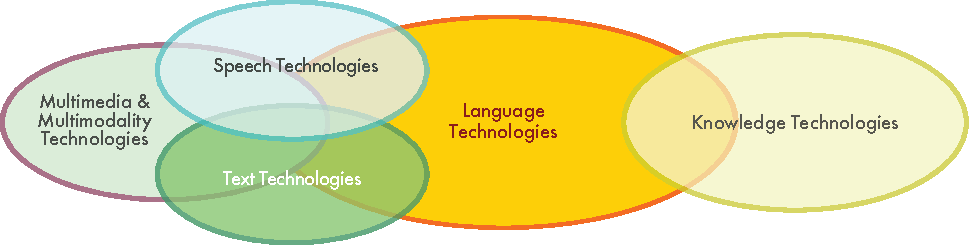
\includegraphics[width=\textwidth]{../_media/english/language_technologies}
\caption{Language technologies} \label{fig: ltincontext_en}
\colorrule{grey3}{\textwidth}{1.5pt} \end{figure*} 

When we communicate, we combine language with other modes of
communication and information media -- for example speaking can
involve gestures and facial expressions. Digital texts link to
pictures and sounds. Movies may contain language in spoken and written
form. In other words, speech and text technologies overlap and
interact with other multimodal communication and multimedia
technologies.\\
In this section, we will discuss the main application areas of
language technology, i.\, e., language checking, web search, speech
interaction, and machine translation. These applications and basic
technologies include: 

\begin{itemize} \item spelling correction \item authoring support
\item computer-assisted language learning \item information retrieval
\item information extraction \item text summarisation \item question
answering \item speech recognition \item speech synthesis
\end{itemize} 

\begin{figure*}[b] \colorrule{grey3}{\textwidth}{1.5pt} \center
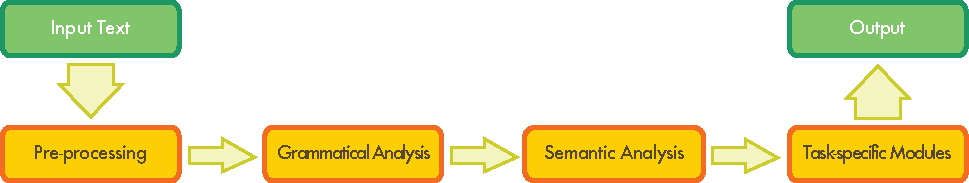
\includegraphics[width=\textwidth]{../_media/english/text_processing_app_architecture}
\caption{A typical text processing architecture} \label{fig:
textprocessingarch_en} \colorrule{grey3}{\textwidth}{1.5pt}
\end{figure*} 

Language technology is an established area of research with an
extensive set of introductory literature. The interested reader is
referred to the following references: \cite{jurafsky-martin01,
manning-schuetze1, lt-world1, lt-survey1, mykowiecka1}. Links to tools
and resources for Polish, which will be mentioned below, are available
on the website \textit{Computational Linguistics in
Poland}~\cite{Clip2}. 

Before discussing the above application areas, we will briefly
describe the architecture of a~typical LT system. 

\subsection{Application Architectures} 

Software applications for language processing typically consist of
several components that mirror different aspects of language.While such applications tend to be very complex, figure~\ref{fig:
textprocessingarch_en} shows a~highly simplified architecture of
a~typical text processing system. The first three modules handle the
structure and meaning of the text input: 

\begin{enumerate} \item Pre-processing: cleans the data, analyses or
removes formatting, detects the input languages, and so on. \item
\textbf{Grammatical analysis}: finds the verb, its objects, modifiers and other sentence elements; detects the sentence structure. \item
\textbf{Semantic analysis}: performs disambiguation (i.\, e., computes
the appropriate meaning of words in a~given context); resolves
anaphora (i.\, e., which pronouns refer to which nouns in the
sentence); represents the meaning of the sentence in
a~machine-readable way. \end{enumerate} 

After analysing the text, task-specific modules can perform other
operations, such as automatic summarisation and database look-ups.
Note that the architectures of the applications are highly simplyfied
and idealised here, to illustrate the complexity of language
technology applications in a~generally understandable way. 

After the introduction of the core application areas, we will give
a~short overview of the situation in LT research and education,
concluding with an overview of (past) funding programs. In the end of
this section, we will present an expert estimation on the situation
regarding core LT tools and resources on a~number of dimensions such
as availability, maturity, or quality in figure~\ref{fig:
lrlttable_en} (p.~\pageref{fig: lrlttable_en}) at the end of this
chapter. This table lists all tools and resources that are boldfaced
in the text. LT support for Polish is also compared to other languages
that are part of this series. 

\subsection{Core Application Areas} 

In this section, we focus on the most important LT tools and
resources, and provide an overview of LT activities in Iceland. 

\subsubsection{Language Checking} 

\begin{figure*}[t] \colorrule{grey3}{\textwidth}{1.5pt} \center
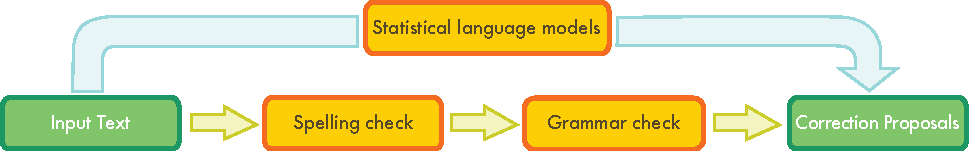
\includegraphics[width=\textwidth]{../_media/english/language_checking}
\caption{Language checking (top: statistical; bottom: rule-based)}
\label{fig: langcheckingaarch_en} \colorrule{grey3}{\textwidth}{1.5pt}
\end{figure*} 

Anyone who has used a~word processor such as Microsoft Word knows that
it has a~spell checker that highlights spelling mistakes and proposes
corrections. 40 years after the first spelling correction program by
Ralph Gorin, language checkers nowadays do not simply compare the list
of extracted words against a~dictionary of correctly spelled words,
but have become increasingly sophisticated. Today these programs are
far more sophisticated. Using language-dependent algorithms for
\textbf{grammatical analysis}, they detect errors related to
morphology (e.\, g., plural formation) as well as syntax--related
errors, such as a~missing verb or a~conflict of verb-subject agreement
(e.\, g., \textit{she *write a~letter}). However, most spell checkers
will not find any errors in the following text \cite{zar1}: 

\begin{verse} I~have a~spelling checker,\\
It came with my PC.\\
It plane lee marks four my revue\\
Miss steaks aye can knot sea. \end{verse} 

Most available spell checkers (including Microsoft Word) will find no
errors in this poem because they mostly look at words in isolation.
However, analysis of larger contexts is needed in many cases, e. g.,
for deciding if a~word such as the “polski” / “Polska” needs
to be written in upper case, as in: 

\begin{itemize} \item Ten tekst został przełożony na polski.
[\textit{This document was written in Polish.}] \item Czytał
„Polskę Zbrojną”. [\textit{He read Polska Zbrojna.}]
\end{itemize} 

This either requires the formulation of language-specific grammar
rules, i. e. a~high degree of expertise and manual labour, or the use
of a~so-called statistical language model (alternatively, grammar
rules might be induced using artificial intelligence methods). Such
models calculate the probability of a~particular word occurring in
a~specific environment (i. e., the preceding and following words). For
example, “polska książka” is a~much more probable word sequence
than “Polska książka”. A~statistical language model can be
automatically derived using a~large amount of (correct) language data
(i. e. a~\textbf{corpus}). Up to now, these approaches have mostly
been developed and evaluated on English language data. However, they
do not necessarily transfer straightforwardly to Polish with its
flexible word order and richer inflection. The rule-based methods have
been used in the open-source proof-reading tool LanguageTool that
incorporates over 1 thousand rules for Polish (the tool can be used in
various word processing systems, such as LibreOffice) \cite{lto1,
Mikowski2010}. 

\boxtext{Language checking is not limited to word processors but also
applies to authoring systems.} 

Accompanying the rising number of technical products, the amount of
technical documentation has rapidly increased over the last decades.
Fearing customer complaints about wrong usage and damage claims
resulting from bad or badly understood instructions, companies have
begun to focus increasingly on the quality of technical documentation,
at the same time targeting the international market. Advances in
natural language processing lead to the development of authoring
support software, which assists the writer of technical documentation
to use vocabulary and sentence structures consistent with certain
rules and (corporate) terminology restrictions. As Polish is rarely
a~source language in such applications, no generic authoring system
has been built especially for Polish. 

Besides spell checkers and authoring support, language checking is
also important in the field of computer-assisted language learning and
is applied to automatically correct queries sent to web search
engines, e. g. Google’s ‘Did you mean…’ suggestions. 

\subsubsection{Web Search} 

\begin{figure*}[t] \colorrule{grey3}{\textwidth}{1.5pt} \center
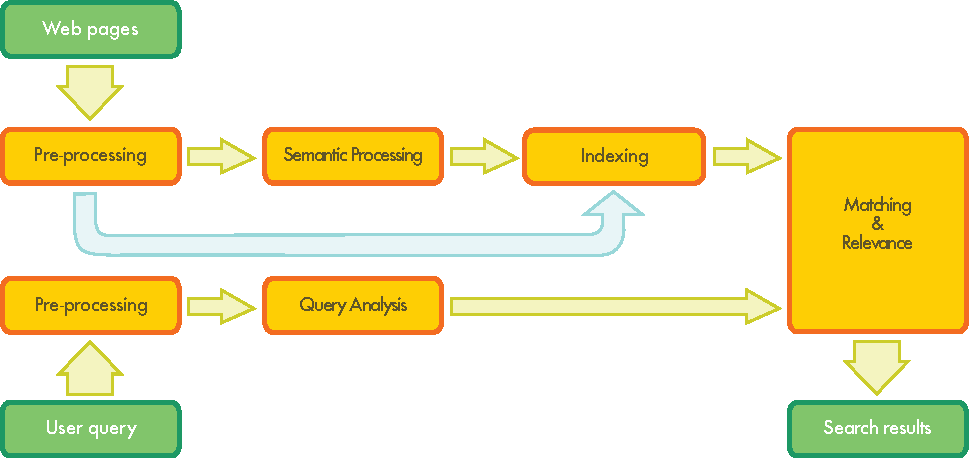
\includegraphics[width=\textwidth]{../_media/english/web_search_architecture}
\caption{Web search} \label{fig: websearcharch_en}
\colorrule{grey3}{\textwidth}{1.5pt} \end{figure*} 

Searching the Web, intranets or digital libraries is probably the most
widely used yet largely underdeveloped language technology application
today. The Google search engine, which started in 1998, now handles
about 80\% of all search queries \cite{spi1}. The search interface and
results page display has not significantly changed since the first
version. In the current version, Google offers spelling correction for
misspelled words and incorporates basic semantic search capabilities
that can improve search accuracy by analysing the meaning of terms in
a~search query context \cite{pc1}. The Google success story shows that
a~large volume of data and efficient indexing techniques can deliver
satisfactory results using a~statistical approach to language
processing. 

However, for a~more sophisticated request for information, integrating
deeper linguistic knowledge is essential. In research labs,
experiments using machine-readable thesauri and ontological language
resources like WordNet (or the Polish equivalent, Słowosieć --
\cite{Slowosiec1, Piasecki2009}) have shown improvements by allowing
to find a~page on the basis of synonyms of the search terms (e. g.
“energia atomowa”, “energia jądrowa”, “energia
nuklearna”, etc.) and even more loosely related terms. 

\boxtext{The next generation of search engines\\
will have to include much more sophisticated language technology.} 

The next generation of search engines will have to include much more
sophisticated language technology, especially to deal with queries
consisting of a~question or other sentence type rather than a~list of
keywords. For the query, \textit{Give me a~list of all companies that
were taken over by other companies in the last five years},
a~syntactic as well as \textbf{semantic analysis} is required. The
system also needs to provide an index to quickly retrieve relevant
documents. A~satisfactory answer will require syntactic parsing to
analyse the grammatical structure of the sentence and determine that
the user wants companies that have been acquired, rather than
companies that have acquired other companies. For the expression
\textit{last five years}, the system needs to determine the relevant
range of years, taking into account the present year. The query then
needs to be matched against a~huge amount of unstructured data to find
the pieces of information that are relevant to the user’s request.
This process is called information retrieval, and involves searching
and ranking relevant documents. To generate a~list of companies, the
system also needs to recognise a~particular string of words in
a~document represents a~company name, using a~process called named
entity recognition. 

A more demanding challenge is matching a~query in one language with
documents in another language. Cross-lingual information retrieval
involves automatically translating the query into all possible source
languages and then translating the results back into the user's target
language. 

Now that data is increasingly found in non-textual formats, there is
a~need for services that deliver multimedia information retrieval by
searching images, audio files and video data. In the case of audio and
video files, a~speech recognition module must convert the speech
content into text (or into a~phonetic representation) that can then be
matched against a~user query. 

In Poland, SMEs like Carrot Search in Poznań successfully develop and
apply search technologies that are able to provide more structured
information than standard engines like Google by clustering the
results in a~language-sensitive way. Polish search engines include
NetSprint and Szukacz. The latter contains a~Polish thesaurus and
stemmer, which enhances the search results. 

\subsubsection{Speech Interaction} 

\begin{figure*}[t] \colorrule{grey3}{\textwidth}{1.5pt} \center
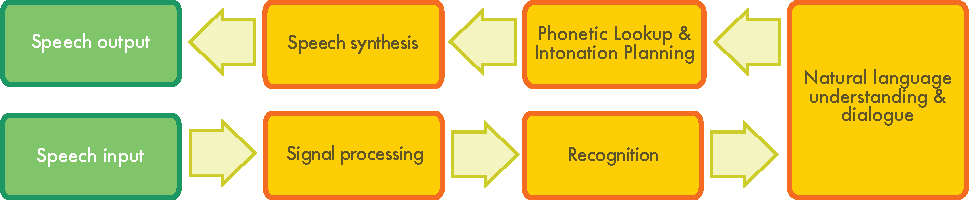
\includegraphics[width=\textwidth]{../_media/english/simple_speech-based_dialogue_architecture}
\caption{Speech-based dialogue system} \label{fig: dialoguearch_en}
\colorrule{grey3}{\textwidth}{1.5pt} \end{figure*} 

Speech interaction technology is used to create interfaces that enable
users to interact in spoken language instead of using a~graphical
display, keyboard and mouse. Today, these voice user interfaces (VUI)
are used for partially or fully automated telephone services provided
by companies to customers, employees or partners. Business domains
that rely heavily on VUIs include banking, supply chain, public
transportation, and telecommunications. Other uses of speech
interaction technology include interfaces to car navigation systems
and the use of spoken language as an alternative to the graphical or
touchscreen interfaces in smartphones. 

Speech interaction technology comprises four technologies: 

\begin{enumerate} \item Automatic \textbf{speech recognition} (ASR)
determines which words are actually spoken in a~given sequence of
sounds uttered by a~user. \item Natural language understanding
analyses the syntactic structure of a~user’s utterance and
interprets it according to the system in question. \item Dialogue
management determines which action to take given the user input and
system functionality. \item \textbf{Speech synthesis} (text-to-speech
or TTS) transforms the system’s reply into sounds for the user.
\end{enumerate} 

One of the major challenges of ASR systems is to accurately recognise
the words a~user utters. This means restricting the range of possible
user utterances to a~limited set of keywords, or manually creating
language models that cover a~large range of natural language
utterances. Using machine learning techniques, language models can
also be generated automatically from \textbf{speech corpora}, i.\, e.,
large collections of speech audio files and text transcriptions.
Restricting utterances usually forces people to use the voice user
interface in a~rigid way and can damage user acceptance; but the
creation, tuning and maintenance of rich language models will
significantly increase costs. VUIs that employ language models and
initially allow a~user to express their intent more flexibly —
prompted by a~\textit{How may I~help you?} greeting — tend to be
automated and are better accepted. 

For the output part of a~VUI, companies tend to use utterances pre-recorded of professional – ideally corporate – speakers a~lot.
For static utterances, in which the wording does not depend on the
particular contexts of use or the personal data of the given user,
this will result in a~rich user experience. However, the more dynamic
content an utterance needs to consider, the more user experience may
suffer from a~poor prosody resulting from concatenating single audio
files. In contrast, today’s TTS systems prove superior, though
optimisable, regarding the prosodic naturalness of dynamic utterances. 

\boxtext{Speech interaction is the basis for interfaces that allow
a~user to interact with spoken language.} 

Regarding the market for speech interaction technology, the last
decade underwent a~strong standardisation of the interfaces between
the different technology components, as well as by standards for
creating particular software artefacts for a~given application. There
also has been strong market consolidation within the last ten years,
particularly in the field of ASR and TTS.~Here, the national markets
in the G20 countries -- i. e. economically strong countries with
a~considerable population -- are dominated by less than 5 players
worldwide, with \textit{Nuance} and \textit{Loquendo} being the most
prominent ones in Europe. 

On the Polish TTS market, the most successful company is \textit{Ivona
}which offers products for other languages as well. However, for
languages with a~smaller number of speakers, commercially employable
ASR and TTS products sometimes do not even exist. Regarding dialogue
management technology and know-how, markets are strongly dominated by
national players, which are usually SMEs. Today’s key players in
Poland are \textit{PrimeSpeech} and \textit{Skrybot}. Rather than
exclusively relying on a~product business based on software licenses,
these companies have positioned themselves mostly as full-service
providers that offer the creation of VUIs as a~system integration
service. Finally, within the domain of \textit{speech} interaction,
a~genuine market for the linguistic core technologies for syntactic
and semantic analysis does not exist yet. 

As for the actual employment of VUIs, demand in Poland has strongly
increased within the last 5 years. This tendency has been driven by
end customers’ increasing demand for customer self service and the
considerable cost optimisation aspect of automated telephone services,
as well as by a~significantly increased acceptance of spoken language
as a~modality for man-machine interaction. 

Looking beyond today’s state of technology, there will be
significant changes due to the spread of smartphones as a~new platform
for managing customer relationships – in addition to the telephone,
Internet, and email channels. This tendency will also affect the
employment of technology for speech interaction. On the one hand,
demand for telephony-based VUIs will decrease, on the long run. On the
other hand, the usage of spoken language as a~user-friendly input
modality for smartphones will gain significant importance. This
tendency is supported by the observable improvement of speaker
independent speech recognition accuracy for speech dictation services
that are already offered as centralised services to smartphone users.
Given this ‘outsourcing’ of the recognition task to the
infrastructure of applications, the application-specific employment of
linguistic core technologies will supposedly gain importance compared
to the present situation. 

\subsubsection{Machine Translation} 

\begin{figure*}[htb] \colorrule{grey3}{\textwidth}{1.5pt} \center
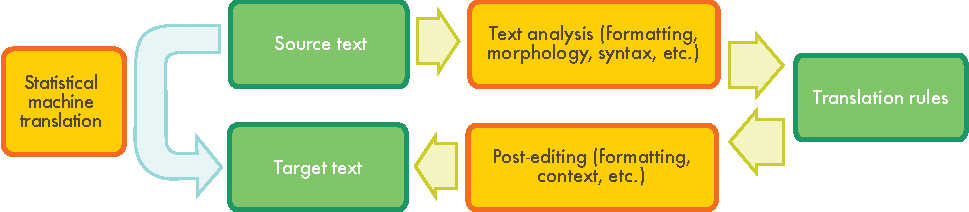
\includegraphics[width=\textwidth]{../_media/english/machine_translation}
\caption{Machine translation (left: statistical; right: rule-based)}
\label{fig: mtarch_en} \colorrule{grey3}{\textwidth}{1.5pt}
\end{figure*} 

The idea of using digital computers for translation of natural
languages came up in 1946 by A.~D.~Booth and was followed by
substantial funding for research in this area in the 1950~s and
beginning again in the 1980~s. Yet \textbf{machine translation} (MT)
still cannot meet its initial promise of across-the-board automated
translation.

\boxtext{At its basic level, Machine Translation simply substitutes
words in one natural language with words in another language.} 

The most basic approach to machine translation is the automatic
replacement of the words in a~text written in one natural language
with the equivalent words of another language. This can be useful in
subject domains that have a~very restricted, formulaic language such
as weather reports. 

However, in order to produce a~good translation of less restricted
texts, larger text units (phrases, sentences, or even whole passages)
need to be matched to their closest counterparts in the target
language. The major difficulty is that human language is ambiguous.
Ambiguity creates challenges on multiple levels, such as word sense
disambiguation at the lexical level (a~\textit{jaguar} is a~brand of
car or an animal) or the assignment of case on the syntactic level,
for example: 

\begin{itemize} \item Policjant zauważył samochód w~zaroślach.
[\textit{The policeman observed the car in the bush.}] \item Policjant
zauważył samochód w~okularach. [\textit{The policeman observed the
car through his glasses}]. \end{itemize} 

One way to build an MT system is to use linguistic rules. For
translations between closely related languages, a~translation using
direct substitution may be feasible in cases such as the above
example. However, rule-based (or linguistic knowledge-driven) systems
often analyse the input text and create an intermediary symbolic
representation from which the target language text can be generated.
The success of these methods is highly dependent on the availability
of extensive lexicons with morphological, syntactic, and semantic
information, and large sets of grammar rules carefully designed by
skilled linguists. This is a~very long and therefore costly process. 

In the late 1980~s when computational power increased and became
cheaper, interest in statistical models for machine translation began
to grow. Statistical models are derived from analysing bilingual text
corpora, \textbf{parallel corpora}, such as the Europarl parallel
corpus, which contains the proceedings of the European Parliament in
21 European languages. Given enough data, statistical MT works well
enough to derive an approximate meaning of a~foreign language text by
processing parallel versions and finding plausible patterns of words.
Unlike knowledge-driven systems, however, statistical (or data-driven)
MT systems often generate ungrammatical output. Data-driven MT is
advantageous because less human effort is required, and it can also
cover special particularities of the language (e.\, g., idiomatic
expressions) that are often ignored in knowledge-driven systems. 

The strengths and weaknesses of knowledge-driven and data-driven
machine translation tend to be complementary, so that nowadays
researchers focus on hybrid approaches that combine both
methodologies. One such approach uses both knowledge-driven and
data-driven systems, together with a~selection module that decides on
the best output for each sentence. However, results for sentences
longer than, say, 12 words, will often be far from perfect. A~more
effective solution is to combine the best parts of each sentence from
multiple outputs; this can be fairly complex, as corresponding parts
of multiple alternatives are not always obvious and need to be
aligned. 

\boxtext{Machine Translation is particularly challenging for the
Polish language.} 

For Polish, machine translation is challenging. The free word order
poses problems for analysis, and extensive inflection is a~challenge
for generating words with proper gender and case markings. 

The leading MT system for Polish is Translatica (Poleng) and it is
widely available. Poleng works with the PWN Scientific Publishers and
uses its extensive dictionaries, including the Oxford PWN
English/Polish dictionary. Translatica is \textbf{rule-based} and
supports Polish, English, German, and Russian. While there is
significant research in this technology in national and international
contexts, data-driven and hybrid systems have been less successful in
business than in research so far. 

However, generic \textbf{statistical} MT systems such as Google
Translate and Bing support Polish to a~considerable degree, especially
in translation from and into English. Nevertheless, for other language
pairs the performance is low and the results are far from
understandable, sometimes even ridiculous. This is due to the scarcity
of the parallel corpora that are used to train statistical MT. 

Provided good adaptation in terms of user-specific terminology and
workflow integration, the use of MT can increase productivity
significantly. Special systems for interactive translation support
were developed e. g. at Poleng (TranslAide) and Studio Gambit (TIGER).
There are also smaller SMEs offering Computer-Aided Translation (CAT)
tools, such as Cafetran. A~special MT system, Thetos, was built to
translate Polish into sign language for the hearing impaired. 

The quality of MT systems is still considered to have huge improvement
potential. Challenges include the adaptability of the language
resources to a~given subject domain or user area and the integration
into existing workflows with term bases and translation memories. In
addition, most of the current systems are English-centred and support
only a~few languages combinations from and into Polish, which leads to
frictions in the total translation workflow, and e. g. forces MT users
to learn different lexicon coding tools for different systems. 

Evaluation campaigns help to compare the quality of MT systems, the
different approaches and the status of the systems for different
language pairs. Figure~\ref{fig: euromatrix_pl} (p.~\pageref{fig:
euromatrix_pl}), which was prepared during the Euromatrix+ project,
shows the pair-wise performances obtained for 22 of the 23 EU
languages (Irish was not compared). The results are ranked according
to a~BLEU score, which indicates higher scores for better translations
\cite{bleu1}. A~human translator would normally achieve a~score of
around 80 points. 

The best results (in green and blue) were achieved by languages that
benefit from a~considerable research effort in coordinated programmes
and the existence of many parallel corpora (e.\, g., English, French,
Dutch, Spanish and German). The languages with poorer results are
shown in red.~These languages either lack such development efforts or
are structurally very different from other languages (e.\, g.,
Hungarian, Maltese and Finnish). 

\subsection{Information management / Language Technology ‘behind the
scenes’} 

Building language technology applications involves a~range of subtasks
that do not always surface at the level of interaction with the user,
but they provide significant service functionalities “behind the
scenes” of the system in question. They all form important research
issues that have now evolved into individual sub-disciplines of
computational linguistics. 

Question answering, for example, is an active area of research for
which annotated corpora have been built and scientific competitions
have been initiated. The concept of question answering goes beyond
keyword-based searches (in which the search engine responds by
delivering a~collection of potentially relevant documents) and enables
users to ask a~concrete question to which the system provides a~single
answer. For example: 

\begin{itemize} 
  \item[] \textit{Question: How old was Neil Armstrong
when he stepped on the moon?} 
  \item[] \textit{Answer: 38.}
\end{itemize} 

While question answering is obviously related to the core area of web
search, it is nowadays an umbrella term for such research issues as
which different types of questions exist, and how they should be
handled; how a~set of documents that potentially contain the answer
can be analysed and compared (do they provide conflicting answers?);
and how specific information (the answer) can be reliably extracted
from a~document without ignoring the context. 

Question answering is in turn related to information extraction (IE),
an area that was extremely popular and influential when computational
linguistics took a~statistical turn in the early 1990~s.~IE aims to
identify specific pieces of information in specific classes of
documents, such as the key players in company takeovers as reported in
newspaper stories. Another common scenario that has been studied is
reports on terrorist incidents. The task here consists of mapping
appropriate parts of the text to a~template that specifies the
perpetrator, target, time, location and results of the incident.
Domain-specific template-filling is the central characteristic of IE,
which makes it another example of a~“behind the scenes” technology
that forms a~well-demarcated research area, which in practice needs to
be embedded into a~suitable application environment. 

\boxtext{Language technology applications often provide significant
service functionalities behind the scenes of larger software systems.} 

Text summarisation and \textbf{text generation} are two borderline
areas that can act either as standalone applications or play
a~supporting role. Summarisation attempts to give the essentials of
a~long text in a~short form, and is one of the features available in
Microsoft Word. It mostly uses a~statistical approach to identify the
“important” words in a~text (i.\, e., words that occur very
frequently in the text in question but less frequently in general
language use) and determine which sentences contain the most of these
“important” words. These sentences are then extracted and put
together to create the summary. In this very common commercial
scenario, summarisation is simply a~form of sentence extraction, and
the text is reduced to a~subset of its sentences. An alternative
approach, for which some research has been carried out, is to generate
brand \emph{new} sentences that do not exist in the source text. This
requires a~certain amount of deeper understanding of the text and
therefore is much less robust. All in all, a~text generator is in most
cases not a~stand-alone application but is embedded into a~larger
software environment, such as the clinical information system where
patient data is collected, stored and processed, and report generation
is just one of many functionalities. 

\boxtext{For the Polish language, research in most text technologies
is much less developed than for the English language.} 

For Polish, the situation in all these research areas is much less
developed than it is for English, where since the 1990~s QA, IE, and
summarisation have been the subject of numerous open competitions,
primarily those organized by DARPA/NIST in the United States. These
have significantly improved the state of the art, but the focus has
always been on English; some competitions have added multilingual
tracks, but Polish was never prominent. Accordingly, there are hardly
any annotated corpora or other resources for these tasks.
Summarisation systems, when using purely statistical methods, are
often to a~good extent language-independent, and thus some research
prototypes are available. For text generation, reusable components
have traditionally been limited to the surface realisation modules
(the {\textquotedbl}generation grammars{\textquotedbl}); again, most
of the available software is designed for English. Prototype
implementations of text generation were created during the development
of MT system that translated Polish into sign language. 

There are other fields in which linguistic technology is being
applied. One of them is plagiarism detection, which uses
language-independent technologies but may be enhanced with search for
simple paraphrases of the text. The most popular Polish application in
this field is the web-based system plagiat .pl, used in most higher
education institutions to ensure originality of
master{\textquotesingle}s theses, as well as to detect document
copyright infringement on the web. 

\subsection[LT Projects]{LT Projects} 

One of the earliest significant projects in computational linguistics
was the creation of the corpus of frequency dictionary of contemporary
Polish by an interdisciplinary team of researchers from the University
of Warsaw. The original purpose of the corpus was to create a~general
frequency dictionary of contemporary Polish. The work started in 1967.
Partial results were published between 1972 and 1977, the completed
dictionary in 1990. The corpus was later augmented in various
respects, both by manual editing and automated procedures. Its design
is comparable to the Brown corpus of English. 

The early efforts included projects that aimed at the creation of
a~representative Polish morphological dictionary. One such project was
POLEX (1993--1996) at Adam Mickiewicz University; another was Słownik
Gramatyczny Języka Polskiego \cite{SGJP} that is included in the
current state-of-the-art morphological analyser for Polish, Morfeusz.
In 2008, an important project plWordNet coordinated by Wrocław
University of Technology (Institute of Applied Informatics)
\cite{Piasecki2009, Slowosiec1}, with the cooperation of Adam
Mickiewicz University (POLNET project), was started in order to build
the first Polish wordnet. The resulting wordnet is one of the biggest
in the world (the coverage in some categories is larger than in
Princeton WordNet), and numerous innovative semi-automatic methods
were used to discover meaning relations on the basis of linguistic
corpora. 

Another important corpus project was the IPI PAN corpus created in
early 2000~s at the Institute of Computer Science of the Polish
Academy of Sciences (ICS PAS). It was the first comprehensible corpus
to be available on the web for Polish \cite{korpus1}. At the same
time, PWN scientific publishers developed their own corpus to be used
for dictionary research, while at the University of Łódź, a~corpus
was built in the Pelcra project. In the next decade, a~follow-up
project, the National Corpus of Polish \cite{nkjp1} was started by
these three institutions and Institute of Polish Language (Cracow) and
it already included some data from their existing resources. The goal
of the project is to create the biggest Polish compiled from a~pool of
over 1 billion words with a~manually annotated 1-million-word part (on
several levels). These annotations will make it possible to prepare
other linguistic resources from it. For example, a~project was started
to build the first Treebank for Polish using the grammatical
annotations from the NKJP corpus. 

Two projects in discourse processing, LUNA (ICS PAS) and
POLINT-112-SMS (Adam Mickiewicz University) were started in the first
decade of 2000~s, to gather spoken language corpora and develop
methods in discourse processing for Polish. The vision of LUNA was to
improve automated telephone systems allowing easy human-machine
interactions through spontaneous and unconstrained speech.
POLINT-112-SMS is focused on information management in emergency
situations. The input data for the system are human-generated text
messages (SMS). They are processed to support decisions in a~crisis
management centre. One of the parts of the project is a~dialogue
maintenance module. 

Polish institutions are also involved in the ongoing CLARIN project
and contribute to the efforts on the technological infrastructure for
language resources and tools, and in FLaReNet, a~European forum to
facilitate interaction among language resources stakeholders. They are
also active in META-NET project. 

There are also at least 2 large ongoing projects financed by the EU
under the Innovative Economy Programme (ATLAS and NEKST), and numerous
other research projects in language technology, including the ones in
the Framework Programme. 

More financial means are necessary to support projects aiming at
developing more sophisticated LT, language corpora and other language
resources. 

\subsection[LT Research and Education]{LT Research and Education} 

Poland has a~number of excellent centres active in the field of
language technology and computational linguistics. Currently, at least
12 Polish universities and research centres are active in the field.
Many of them offer courses in the field of language technology
\cite{centers1}. 

Apart from the universities, major research projects are carried out
by the language technology group of the Institute of the Computer
Sciences of the Polish Academy of Sciences (ICS PAS). 

Polish associations active in the field of language technology are
Polskie Towarzystwo Informatyczne and Polskie Towarzystwo Fonetyczne. 

LT as a~field of research faces the following problems: 

\begin{itemize} \item Since researchers are part of different
communities they meet in several separate conferences and have
different meetings and boards. Hence, there is no single conference at
which one can meet all stakeholders. \item Computational linguistics
is still seen as an ‘exotic’ topic, which has not acquired a~fixed
place in the faculty system yet, and hence is located in different
faculties, e. g. the computer science faculties or in the humanities.
\item Research topics dealt with are overlapping only partially.
\end{itemize} 

\subsection{Availability of Tools and Resources} 

Figure~\ref{fig: lrlttable_en} provides a~rating for language
technology support for the Polish language. This rating of existing
tools and resources was generated by leading experts in the field who
provided estimates based on a~scale from 0 (very low) to 6 (very high)
using seven criteria. 

\begin{figure*}[htb]
\centering
%\begin{tabular}{>{\columncolor{orange1}}p{.33\linewidth}ccccccc} % ORIGINAL
\begin{tabular}{>{\columncolor{orange1}}p{.33\linewidth}@{\hspace*{6mm}}c@{\hspace*{6mm}}c@{\hspace*{6mm}}c@{\hspace*{6mm}}c@{\hspace*{6mm}}c@{\hspace*{6mm}}c@{\hspace*{6mm}}c}
\rowcolor{orange1}
 \cellcolor{white}&\begin{sideways}\makecell[l]{Quantity}\end{sideways}
&\begin{sideways}\makecell[l]{\makecell[l]{Availability} }\end{sideways} &\begin{sideways}\makecell[l]{Quality}\end{sideways}
&\begin{sideways}\makecell[l]{Coverage}\end{sideways} &\begin{sideways}\makecell[l]{Maturity}\end{sideways} &\begin{sideways}\makecell[l]{Sustainability~~~}\end{sideways} &\begin{sideways}\makecell[l]{Adaptability}\end{sideways} \\ \addlinespace
\multicolumn{8}{>{\columncolor{orange2}}l}{Language Technology: Tools, Technologies and Applications} \\ \addlinespace
Speech Recognition & 1 & 2 & 3 & 4 & 3 & 2 & 4\\ \addlinespace
Speech Synthesis & 4 & 3 & 6 & 5 & 4 & 4 & 3\\ \addlinespace
Grammatical analysis & 4 & 4,5 & 4,5 & 4,5 & 4 & 4 & 3\\ \addlinespace
Semantic analysis & 1 & 1 & 3 & 1 & 1 & 2 & 2\\ \addlinespace
Text generation & 1 & 1 & 1 & 1 & 1 & 1 & 2\\ \addlinespace
Machine translation & 3 & 4 & 3 & 3 & 3 & 4 & 3\\ \addlinespace
\multicolumn{8}{>{\columncolor{orange2}}l}{Language Resources: Resources, Data and Knowledge Bases} \\ \addlinespace
Text corpora & 3 & 2 & 4 & 4 &  5 & 5 & 3\\ \addlinespace
Speech corpora & 1 & 0 & 3 & 3 & 2 & 2 & 2\\ \addlinespace
Parallel corpora & 3 & 1 & 4 & 4 & 5 & 5 & 5\\ \addlinespace
Lexical resources & 3 & 3 & 4 & 4 & 4 & 4 & 3\\ \addlinespace
Grammars & 3 & 2 & 4 & 4 & 3 & 2 &  2\\
\end{tabular}
\caption{State of language technology support for Polish}
\label{fig:lrlttable_en}
\end{figure*}


The key results for Polish language technology can be summed up as
follows: 

\begin{itemize} \item For Polish, discourse corpora or advanced
discourse processing are not widely available. Multimodal corpora are
in preparation. \item Many of the resources lack standardization, i.
e. even if they exist, sustainability is not given; concerted programs
and initiatives are needed to standardise data and interchange
formats. \item Semantics is more difficult to process than syntax;
text semantics is more difficult to process than word and sentence
semantics. \item The more semantics a~tool takes into account, the
more difficult it is to find the right data; more efforts for
supporting deep processing are needed. \item Standards do exist for
semantics in the sense of world knowledge (RDF, OWL, etc.); they are,
however, not easily applicable to NLP tasks. \item Speech processing,
specially speech synthesis, is currently more mature than NLP for
written text. \item Research was successful in designing particular
high quality software, but it is nearly impossible to come up with
sustainable and standardized solutions given the current funding
situations. \item Polish lacks large, balanced and more easily
available parallel corpora, including large parallel corpora for
related languages such as Czech or Polish. \item For many purposes,
bilingual and multilingual dictionaries that include not only
translations but also valency information seem indispensable. These
need to be built, as standard dictionaries usually omit this kind of
annotation. \item Large and widely available ontological resources for
Polish are needed for many applications. Currently available
ontologies are relatively small, based on OpenCyc or on Polish
OpenThesaurus. A~Polish version of DBPedia is in preparation.
\end{itemize} 

\subsection{Cross-language comparison} The current state of LT support
varies considerably from one language community to another. In order
to compare the situation between languages, this section will present
an evaluation based on two sample application areas (machine
translation and speech processing) and one underlying technology (text
analysis), as well as basic resources needed for building LT
applications. The languages were categorised using the following
five-point scale: 

\begin{enumerate} \item Excellent support \item Good support \item
Moderate support \item Fragmentary support \item Weak or no support
\end{enumerate} 

LT support was measured according to the following criteria: 

\textbf{Speech Processing:} Quality of existing speech recognition
technologies, quality of existing speech synthesis technologies,
coverage of domains, number and size of existing speech corpora,
amount and variety of available speech-based applications. 

\textbf{Machine Translation:} Quality of existing MT technologies,
number of language pairs covered, coverage of linguistic phenomena and
domains, quality and size of existing parallel corpora, amount and
variety of available MT applications. 

\textbf{Text Analysis:} Quality and coverage of existing text analysis
technologies (morphology, syntax, semantics), coverage of linguistic
phenomena and domains, amount and variety of available applications,
quality and size of existing (annotated) text corpora, quality and
coverage of existing lexical resources (e.\, g., WordNet) and
grammars. 

\textbf{Resources:} Quality and size of existing text corpora, speech
corpora and parallel corpora, quality and coverage of existing lexical
resources and grammars. 

\subsection{Conclusions} 

\emph{In this series of white papers, we have made an important effort
by assessing the language technology support for 30 European
languages, and by providing a~high-level comparison across these
languages. By identifying the gaps, needs and deficits, the European
language technology community and its related stakeholders are now in
a~position to design a~large scale research and development programme
aimed at building a~truly multilingual, technology-enabled
communication across Europe.} 

The results of this white paper series show that there is a~dramatic
difference in language technology support between the various European
languages. While there are good quality software and resources
available for some languages and application areas, others, usually
smaller languages, have substantial gaps. Many languages lack basic
technologies for text analysis and the essential resources. Others
have basic tools and resources but the implementation of for example
semantic methods is still far away. Therefore a~large-scale effort is
needed to attain the ambitious goal of providing high-quality language
technology support for all European languages, for example through
high quality machine translation. 

There is also a~lack of continuity in research and development
funding. Short-term coordinated programmes tend to alternate with
periods of sparse or zero funding. In addition, there is an overall
lack of coordination with programmes in other EU countries and at the
European Commission level. 

We can therefore conclude that there is a~desperate need for a~large,
coordinated initiative focused on overcoming the differences in
language technology readiness for European languages as a~whole. 

The long term goal of META-NET is to enable the creation of high-quality language technology for all languages. This requires all stakeholders -- in politics, research, business, and society -- to unite their efforts. The resulting technology will help tear down existing barriers and build bridges between Europe’s languages, paving the way for political and economic unity through cultural diversity. 
\end{multicols}
\clearpage
\begin{figure*}[t]
  \small
  \centering
  \begin{tabular}
  { % defines color for each column.
  >{\columncolor{corange5}}p{.13\linewidth}@{\hspace{.040\linewidth}}
  >{\columncolor{corange4}}p{.13\linewidth}@{\hspace{.040\linewidth}}
  >{\columncolor{corange3}}p{.13\linewidth}@{\hspace{.040\linewidth}}
  >{\columncolor{corange2}}p{.13\linewidth}@{\hspace{.040\linewidth}}
  >{\columncolor{corange1}}p{.13\linewidth} 
  }
  \multicolumn{1}{>{\columncolor{white}}c@{\hspace{.040\linewidth}}}{\textbf{Excellent}} & 
  \multicolumn{1}{@{}>{\columncolor{white}}c@{\hspace{.040\linewidth}}}{\textbf{Good}} &
  \multicolumn{1}{@{}>{\columncolor{white}}c@{\hspace{.040\linewidth}}}{\textbf{Moderate}} &
  \multicolumn{1}{@{}>{\columncolor{white}}c@{\hspace{.040\linewidth}}}{\textbf{Fragmentary}} &
  \multicolumn{1}{@{}>{\columncolor{white}}c}{\textbf{Weak/no}} \\ 
  \multicolumn{1}{>{\columncolor{white}}c@{\hspace{.040\linewidth}}}{\textbf{support}} & 
  \multicolumn{1}{@{}>{\columncolor{white}}c@{\hspace{.040\linewidth}}}{\textbf{support}} &
  \multicolumn{1}{@{}>{\columncolor{white}}c@{\hspace{.040\linewidth}}}{\textbf{support}} &
  \multicolumn{1}{@{}>{\columncolor{white}}c@{\hspace{.040\linewidth}}}{\textbf{support}} &
  \multicolumn{1}{@{}>{\columncolor{white}}c}{\textbf{support}} \\ \addlinespace
  
& \vspace*{0.5mm}English
& \vspace*{0.5mm}
Czech \newline 
Dutch \newline 
Finnish \newline 
French \newline 
German \newline   
Italian \newline  
Portuguese \newline 
Spanish \newline
& \vspace*{0.5mm}Basque \newline 
Bulgarian \newline 
Catalan \newline 
Danish \newline 
Estonian \newline 
Galician\newline 
Greek \newline  
Hungarian  \newline
Irish \newline  
Norwegian \newline 
\textbf{Polish} \newline 
Serbian \newline 
Slovak \newline 
Slovene \newline 
Swedish \newline
& \vspace*{0.5mm}
Croatian \newline 
Icelandic \newline  
Latvian \newline 
Lithuanian \newline 
Maltese \newline 
Romanian\\
\end{tabular}
\caption{Speech processing: state of language technology support for 30 European languages}
\label{fig:speech_cluster_en}
\end{figure*}


\begin{figure*}[b]
  \small
  \centering
  \begin{tabular}
  { % defines color for each column.
  >{\columncolor{corange5}}p{.13\linewidth}@{\hspace{.040\linewidth}}
  >{\columncolor{corange4}}p{.13\linewidth}@{\hspace{.040\linewidth}}
  >{\columncolor{corange3}}p{.13\linewidth}@{\hspace{.040\linewidth}}
  >{\columncolor{corange2}}p{.13\linewidth}@{\hspace{.040\linewidth}}
  >{\columncolor{corange1}}p{.13\linewidth} 
  }
  \multicolumn{1}{>{\columncolor{white}}c@{\hspace{.040\linewidth}}}{\textbf{Excellent}} & 
  \multicolumn{1}{@{}>{\columncolor{white}}c@{\hspace{.040\linewidth}}}{\textbf{Good}} &
  \multicolumn{1}{@{}>{\columncolor{white}}c@{\hspace{.040\linewidth}}}{\textbf{Moderate}} &
  \multicolumn{1}{@{}>{\columncolor{white}}c@{\hspace{.040\linewidth}}}{\textbf{Fragmentary}} &
  \multicolumn{1}{@{}>{\columncolor{white}}c}{\textbf{Weak/no}} \\ 
  \multicolumn{1}{>{\columncolor{white}}c@{\hspace{.040\linewidth}}}{\textbf{support}} & 
  \multicolumn{1}{@{}>{\columncolor{white}}c@{\hspace{.040\linewidth}}}{\textbf{support}} &
  \multicolumn{1}{@{}>{\columncolor{white}}c@{\hspace{.040\linewidth}}}{\textbf{support}} &
  \multicolumn{1}{@{}>{\columncolor{white}}c@{\hspace{.040\linewidth}}}{\textbf{support}} &
  \multicolumn{1}{@{}>{\columncolor{white}}c}{\textbf{support}} \\ \addlinespace
  
& \vspace*{0.5mm} English 
& \vspace*{0.5mm} 
French \newline 
Spanish
& \vspace*{0.5mm}
Catalan \newline 
Dutch \newline 
German \newline 
Hungarian \newline
Italian \newline 
\textbf{Polish} \newline 
Romanian \newline 
& \vspace*{0.5mm}Basque \newline 
Bulgarian \newline 
Croatian \newline 
Czech \newline
Danish \newline 
Estonian \newline 
Finnish \newline 
Galician \newline 
Greek \newline 
Icelandic \newline 
Irish \newline 
Latvian \newline 
Lithuanian \newline 
Maltese \newline 
Norwegian \newline 
Portuguese \newline 
Serbian \newline 
Slovak \newline 
Slovene \newline 
Swedish \newline 
\end{tabular}
\caption{Machine translation: state of language technology support for 30 European languages}
\label{fig:mt_cluster_en}
\end{figure*}


\begin{figure*}[t]
  \small
  \centering
  \begin{tabular}
  { % defines color for each column.
  >{\columncolor{corange5}}p{.13\linewidth}@{\hspace{.040\linewidth}}
  >{\columncolor{corange4}}p{.13\linewidth}@{\hspace{.040\linewidth}}
  >{\columncolor{corange3}}p{.13\linewidth}@{\hspace{.040\linewidth}}
  >{\columncolor{corange2}}p{.13\linewidth}@{\hspace{.040\linewidth}}
  >{\columncolor{corange1}}p{.13\linewidth} 
  }
  \multicolumn{1}{>{\columncolor{white}}c@{\hspace{.040\linewidth}}}{\textbf{Excellent}} & 
  \multicolumn{1}{@{}>{\columncolor{white}}c@{\hspace{.040\linewidth}}}{\textbf{Good}} &
  \multicolumn{1}{@{}>{\columncolor{white}}c@{\hspace{.040\linewidth}}}{\textbf{Moderate}} &
  \multicolumn{1}{@{}>{\columncolor{white}}c@{\hspace{.040\linewidth}}}{\textbf{Fragmentary}} &
  \multicolumn{1}{@{}>{\columncolor{white}}c}{\textbf{Weak/no}} \\ 
  \multicolumn{1}{>{\columncolor{white}}c@{\hspace{.040\linewidth}}}{\textbf{support}} & 
  \multicolumn{1}{@{}>{\columncolor{white}}c@{\hspace{.040\linewidth}}}{\textbf{support}} &
  \multicolumn{1}{@{}>{\columncolor{white}}c@{\hspace{.040\linewidth}}}{\textbf{support}} &
  \multicolumn{1}{@{}>{\columncolor{white}}c@{\hspace{.040\linewidth}}}{\textbf{support}} &
  \multicolumn{1}{@{}>{\columncolor{white}}c}{\textbf{support}} \\ \addlinespace


& \vspace*{0.5mm}English
& \vspace*{0.5mm}
  Dutch \newline 
  French \newline 
  German \newline 
  Italian \newline 
  Spanish
& \vspace*{0.5mm}Basque \newline 
  Bulgarian \newline 
  Catalan \newline 
  Czech \newline 
  Danish \newline 
  Finnish \newline 
  Galician \newline 
  Greek \newline 
  Hungarian \newline 
  Norwegian \newline 
  \textbf{Polish} \newline 
  Portuguese \newline 
  Romanian \newline 
  Slovak \newline 
  Slovene \newline 
  Swedish \newline 
& \vspace*{0.5mm}
  Croatian \newline 
  Estonian \newline 
  Icelandic \newline 
  Irish \newline 
  Latvian \newline 
  Lithuanian \newline 
  Maltese \newline 
  Serbian \\
  \end{tabular}
\caption{Text analysis: state of language technology support for 30 European languages}
\label{fig:text_cluster_en}
\end{figure*}


\begin{figure*}[b]
  \small
  \centering
  \begin{tabular}
  { % defines color for each column.
  >{\columncolor{corange5}}p{.13\linewidth}@{\hspace{.040\linewidth}}
  >{\columncolor{corange4}}p{.13\linewidth}@{\hspace{.040\linewidth}}
  >{\columncolor{corange3}}p{.13\linewidth}@{\hspace{.040\linewidth}}
  >{\columncolor{corange2}}p{.13\linewidth}@{\hspace{.040\linewidth}}
  >{\columncolor{corange1}}p{.13\linewidth} 
  }
  \multicolumn{1}{>{\columncolor{white}}c@{\hspace{.040\linewidth}}}{\textbf{Excellent}} & 
  \multicolumn{1}{@{}>{\columncolor{white}}c@{\hspace{.040\linewidth}}}{\textbf{Good}} &
  \multicolumn{1}{@{}>{\columncolor{white}}c@{\hspace{.040\linewidth}}}{\textbf{Moderate}} &
  \multicolumn{1}{@{}>{\columncolor{white}}c@{\hspace{.040\linewidth}}}{\textbf{Fragmentary}} &
  \multicolumn{1}{@{}>{\columncolor{white}}c}{\textbf{Weak/no}} \\ 
  \multicolumn{1}{>{\columncolor{white}}c@{\hspace{.040\linewidth}}}{\textbf{support}} & 
  \multicolumn{1}{@{}>{\columncolor{white}}c@{\hspace{.040\linewidth}}}{\textbf{support}} &
  \multicolumn{1}{@{}>{\columncolor{white}}c@{\hspace{.040\linewidth}}}{\textbf{support}} &
  \multicolumn{1}{@{}>{\columncolor{white}}c@{\hspace{.040\linewidth}}}{\textbf{support}} &
  \multicolumn{1}{@{}>{\columncolor{white}}c}{\textbf{support}} \\ \addlinespace
    
& \vspace*{0.5mm}English
& \vspace*{0.5mm} 
    Czech \newline 
    Dutch \newline 
    French \newline 
    German \newline 
    Hungarian \newline
    Italian \newline
    \textbf{Polish} \newline
    Spanish \newline
    Swedish \newline 
& \vspace*{0.5mm} Basque\newline 
    Bulgarian\newline 
    Catalan \newline 
    Croatian \newline 
    Danish \newline 
    Estonian \newline 
    Finnish \newline 
    Galician \newline 
    Greek \newline 
    Norwegian \newline 
    Portuguese \newline 
    Romanian \newline 
    Serbian \newline 
    Slovak \newline 
    Slovene \newline
&  \vspace*{0.5mm}
    Icelandic \newline 
    Irish \newline 
    Latvian \newline 
    Lithuanian \newline 
    Maltese  \\
  \end{tabular}
  \caption{Speech and text resources: State of support for 30 European languages}  
  \label{fig:resources_cluster_en}
\end{figure*}


\clearpage 

\ssection[About META-NET]{About META-NET} 

\begin{multicols}{2} 

META-NET is a~Network of Excellence partially funded by the European
Commission. The network currently consists of 54 research centres in
33 European countries \cite{rehm2011}. META-NET forges META, the
Multilingual Europe Technology Alliance, a~growing community of
language technology professionals and organisations in Europe.
META-NET fosters the technological foundations for a~truly
multilingual European information society that: 

\begin{itemize} \item makes communication and cooperation possible
across languages; \item grants all Europeans equal access to
information and knowledge regardless of their language; \item builds
upon and advances functionalities of networked information technology.
\end{itemize} 

The network supports a~Europe that unites as a~single digital market
and information space. It stimulates and promotes multilingual
technologies for all European languages. These technologies support
automatic translation, content production, information processing and
knowledge management for a~wide variety of subject domains and
applications. They also enable intuitive language-based interfaces to
technology ranging from household electronics, machinery and vehicles
to computers and robots. Launched on 1 February 2010, META-NET has
already conducted various activities in its three lines of action
META-VISION, META-SHARE and META-RESEARCH. 

\textbf{META-VISION} fosters a~dynamic and influential stakeholder
community that unites around a~shared vision and a~common strategic
research agenda (SRA). The main focus of this activity is to build
a~coherent and cohesive LT community in Europe by bringing together
representatives from highly fragmented and diverse groups of
stakeholders. The present White Paper was prepared together with
volumes for 29 other languages. The shared technology vision was
developed in three sectorial Vision Groups. The META Technology
Council was established in order to discuss and to prepare the SRA
based on the vision in close interaction with the entire LT community. 

\textbf{META-SHARE} creates an open, distributed facility for
exchanging and sharing resources. The peer-to-peer network of
repositories will contain language data, tools and web services that
are documented with high-quality metadata and organised in
standardised categories. The resources can be readily accessed and
uniformly searched. The available resources include free, open source
materials as well as restricted, commercially available, fee-based
items. 

\textbf{META-RESEARCH} builds bridges to related technology fields.
This activity seeks to leverage advances in other fields and to
capitalise on innovative research that can benefit language
technology. In particular, the action line focuses on conducting
leading-edge research in machine translation, collecting data,
preparing data sets and organising language resources for evaluation
purposes; compiling inventories of tools and methods; and organising
workshops and training events for members of the community.\\ 

\textbf{\centerline{office@meta-net.eu -- http://www.meta-net.eu}}
\end{multicols} \vfill 

\cleardoublepage 

\appendix \addtocontents{toc}{\protect\bigskip} 

\bsection[Bibliografia -- References]{Bibliografia --- References}
\bibliographystyle{unsrt} \bibliography{polish_references}

\cleardoublepage 

\bsection[Członkowie sieci META-NET --- META-NET Members]{Członkowie
sieci META-NET --- META-NET \ \ \ \ \ \ \ Members}
\label{metanetmembers} 

\small \begin{longtable}{llp{115mm}} Austria &
\textcolor{grey1}{Austria} & Zentrum für Translationswissenschaft,
Universität Wien: Gerhard Budin\\
\addlinespace Belgia & \textcolor{grey1}{Belgium} & Computational
Linguistics and Psycholinguistics Research Centre, University of
Antwerp: Walter Daelemans\\
\addlinespace & & Centre for Processing Speech and Images, University
of Leuven: Dirk van Compernolle\\
\addlinespace Bułgaria & \textcolor{grey1}{Bulgaria} & Institute for
Bulgarian Language, Bulgarian Academy of Sciences: Svetla Koeva\\
\addlinespace Chorwacja & \textcolor{grey1}{Croatia} & Institute of
Linguistics, Faculty of Humanities and Social Science, University of
Zagreb: Marko Tadić\\
\addlinespace Cypr & \textcolor{grey1}{Cyprus} & Language Centre,
School of Humanities: Jack Burston\\
\addlinespace Czechy & \textcolor{grey1}{Czech Republic} & Institute
of Formal and Applied Linguistics, Charles University in Prague: Jan
Hajič\\
\addlinespace Dania & \textcolor{grey1}{Denmark} & Centre for Language
Technology, University of Copenhagen: \newline Bolette Sandford
Pedersen, Bente Maegaard\\
\addlinespace Estonia & \textcolor{grey1}{Estonia} & Institute of
Computer Science, University of Tartu: Tiit Roosmaa, Kadri Vider\\
\addlinespace Finlandia & \textcolor{grey1}{Finland} & Computational
Cognitive Systems Research Group, Aalto University: Timo Honkela\\
\addlinespace & & Department of Modern Languages, University of
Helsinki:\newline Kimmo Koskenniemi, Krister Lindén\\
\addlinespace Francja & \textcolor{grey1}{France} & Centre National de
la Recherche Scientifique, Laboratoire d'Informatique pour la
Mécanique et les Sciences de l'Ingénieur and Institute for
Multilingual and Multimedia Information: Joseph Mariani\\
\addlinespace & & Evaluations and Language Resources Distribution
Agency: Khalid Choukri\\
\addlinespace Grecja & \textcolor{grey1}{Greece} & R. C. “Athena”,
Institute for Language and Speech Processing: Stelios Piperidis\\
\addlinespace Hiszpania & \textcolor{grey1}{Spain} & Barcelona Media:
Toni Badia, Maite Melero\\
\addlinespace & & Institut Universitari de Lingüística Aplicada,
Universitat Pompeu Fabra: Núria Bel\\
\addlinespace & & Aholab Signal Processing Laboratory, University of
the Basque Country:\newline Inma Hernaez Rioja\\
\addlinespace & & Center for Language and Speech Technologies and
Applications, Universitat Politècnica de Catalunya: Asunción Moreno
\\
\addlinespace & & Department of Signal Processing and Communications,
University of Vigo:\newline Carmen García Mateo\\
\addlinespace Holandia & \textcolor{grey1}{Netherlands} & Utrecht
Institute of Linguistics, Utrecht University: Jan Odijk\\
\addlinespace & & Computational Linguistics, University of Groningen:
Gertjan van Noord\\
\addlinespace Irlandia & \textcolor{grey1}{Ireland} & School of
Computing, Dublin City University: Josef van Genabith\\
\addlinespace Islandia & \textcolor{grey1}{Iceland} & School of
Humanities, University of Iceland: Eiríkur Rögnvaldsson\\
\addlinespace Litwa & \textcolor{grey1}{Lithuania} & Institute of the
Lithuanian Language: Jolanta Zabarskaitė\\
\addlinespace Luksemburg & \textcolor{grey1}{Luxembourg} & Arax Ltd.:
Vartkes Goetcherian\\
\addlinespace Łotwa & \textcolor{grey1}{Latvia} & Tilde: Andrejs
Vasiļjevs\\
\addlinespace & & Institute of Mathematics and Computer Science,
University of Latvia: Inguna Skadiņa\\
\addlinespace Malta & \textcolor{grey1}{Malta} & Department
Intelligent Computer Systems, University of Malta: Mike Rosner\\
\addlinespace Niemcy & \textcolor{grey1}{Germany} & Language
Technology Lab, DFKI: Hans Uszkoreit, Georg Rehm\\
\addlinespace & & Human Language Technology and Pattern Recognition,
RWTH Aachen University: Hermann Ney\\
\addlinespace & & Department of Computational Linguistics, Saarland
University: Manfred Pinkal\\
\addlinespace Norwegia & \textcolor{grey1}{Norway} & Department of
Linguistic, University of Bergen: Koenraad De Smedt\\
\addlinespace & & Department of Informatics, Language Technology
Group, University of Oslo:\newline Stephan Oepen\\
\addlinespace Polska & \textcolor{grey1}{Poland} & Institute of
Computer Science, Polish Academy of Sciences: \newline Adam
Przepiórkowski, Maciej Ogrodniczuk\\
\addlinespace & & University of Łódź: Barbara
Lewandowska-Tomaszczyk, Piotr Pęzik\\
\addlinespace & & Department of Computer Linguistics and Artificial
Intelligence, Adam Mickiewicz University: Zygmunt Vetulani\\
\addlinespace Portugalia & \textcolor{grey1}{Portugal} & University of
Lisbon: António Branco, Amália Mendes\\
\addlinespace & & Spoken Language Systems Laboratory, Institute for
Systems Engineering and Computers: Isabel Trancoso\\
\addlinespace Rumunia & \textcolor{grey1}{Romania} & Research
Institute for Artificial Intelligence, Romanian Academy of
Sciences:\newline Dan Tufiș\\
\addlinespace & & Faculty of Computer Science, University Alexandru
Ioan Cuza of Iași: Dan Cristea\\
\addlinespace Serbia & \textcolor{grey1}{Serbia} & University of
Belgrade, Faculty of Mathematics: Duško Vitas, Cvetana
Krstev,\newline Ivan Obradović\\
\addlinespace & & Pupin Institute: Sanja Vranes\\
\addlinespace Szwajcaria & \textcolor{grey1}{Switzerland} & Idiap
Research Institute: Hervé Bourlard\\
\addlinespace Szwecja & \textcolor{grey1}{Sweden} & Department of
Swedish, University of Gothenburg: Lars Borin\\
\addlinespace Słowacja & \textcolor{grey1}{Slovakia} & Ľudovít
Štúr Institute of Linguistics, Slovak Academy of Sciences: Radovan
Garabík\\
\addlinespace Słowenia & \textcolor{grey1}{Slovenia} & Jožef Stefan
Institute: Marko Grobelnik\\
\addlinespace Wielka Brytania & \textcolor{grey1}{UK} & School of
Computer Science, University of Manchester: Sophia Ananiadou\\
\addlinespace & & Institute for Language, Cognition and Computation,
Center for Speech Technology Research, University of Edinburgh: Steve
Renals\\
\addlinespace & & Research Institute of Informatics and Language
Processing, University of Wolverhampton: Ruslan Mitkov\\
\addlinespace && Department of Computer Science, University of
Sheffield: Rob Gaizauskas\\
\addlinespace Węgry & \textcolor{grey1}{Hungary} & Research Institute
for Linguistics, Hungarian Academy of Sciences: Tamás Váradi\\
\addlinespace & & Department of Telecommunications and Media
Informatics, Budapest University of Technology and Economics: Géza
Németh, Gábor Olaszy\\
\addlinespace Włochy & \textcolor{grey1}{Italy} & Consiglio Nazionale
delle Ricerche, Istituto di Linguistica Computazionale \newline
“Antonio Zampolli”: Nicoletta Calzolari\\
\addlinespace & & Human Lang. Technology, Fondazione Bruno Kessler:
Bernardo Magnini\\
\addlinespace \end{longtable} \normalsize 

\renewcommand*{\figureformat}{} \renewcommand*{\captionformat}{} 

\begin{figure*}[htb] \colorrule{grey3}{\textwidth}{1.5pt} \center
  \fbox{-- META-NET group picture omitted to keep the size of the PDF file small. --}
  %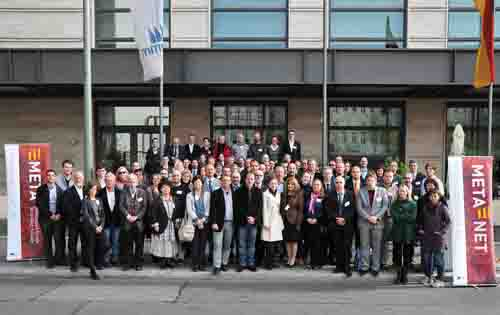
\includegraphics[width=\textwidth]{../_media/meta-net_team.jpg}
  \caption{Około 100 ekspertów ds. technologii językowych --
przedstawicieli krajów i~języków reprezentowanych w~sieci META-NET
-- omawiało i~zatwierdzało podstawowe rezultaty zawarte w~raportach
z~serii META-NET, a~także jego wydźwięk, na spotkaniu w~Berlinie
(Niemcy) w~dniach 21--22 października 2011. --
  \textcolor{grey1}{About 100 language technology experts --
representatives of the countries and languages represented in META-NET
-- discussed and finalised the key results and messages of the White
Paper Series at a~META-NET meeting in Berlin, Germany, on October
21/22, 2011.}} \medskip \colorrule{grey3}{\textwidth}{1.5pt}
\end{figure*} 

\cleardoublepage 

\bsection[Seria raportów META-NET -- The META-NET White Paper
Series]{Seria raportów META-NET --- The META-NET\ \ \ \ \ \ White
Paper Series} \label{whitepaperseries} 

\vspace*{-5mm}
\centering
  \setlength{\tabcolsep}{2em}
  \begin{tabularx}{\textwidth}{lllll} \toprule\addlinespace
  %\begin{tabulary}{170mm}{LLL} \toprule
&angielski& English& English& \\
&baskijski& Basque& euskara& \\
&bułgarski& Bulgarian& български& \\
&chorwacki& Croatian& hrvatski& \\
&czeski& Czech& čeština& \\
&duński& Danish& dansk& \\
&estoński& Estonian& eesti& \\
&fiński& Finnish& suomi& \\
&francuski& French& français& \\
&galisyjski& Galician& galego& \\
&grecki& Greek & ελληνικά \\
&hiszpański& Spanish & espanol& \\
&irlandzki& Irish& Gaeilge& \\
&islandzki& Icelandic& íslenska& \\
&kataloński& Catalan& catala& \\
&litewski& Lithuanian& lietuvi\k{u} kalba& \\
&łotewski& Latvian& latviešu valoda& \\
&maltański& Maltese& Malti& \\
&niderlandzki& Dutch& Nederlands& \\
&niemiecki& German& Deutsch& \\
&norweski – bókmál& Norwegian Bokmal& bokmal& \\
&norweski – nynorsk& Norwegian Nynorsk& nynorsk& \\
&polski& Polish& polski& \\
&portugalski& Portuguese& portugues& \\
&rumuński& Romanian& română& \\
&serbski& Serbian& српски& \\
&słowacki& Slovak& slovenčina& \\
&słoweński& Slovene& slovenščina& \\
&szwedzki& Swedish& svenska& \\
&węgierski& Hungarian& magyar& \\
&włoski& Italian& italiano& \\
\bottomrule
\end{tabularx}
